\documentclass[superscriptaddress,onecolumn,floatfix]{revtex4-2}

\usepackage{graphicx}
\usepackage{epsfig}
\usepackage{color}
\usepackage{amssymb}
\usepackage{amsmath}
\usepackage{array}
\usepackage[loose]{units}
\usepackage[french]{babel}
\usepackage[unicode,colorlinks=true]{hyperref}
\usepackage{cleveref}
\usepackage{braket}
\usepackage[caption=false]{subfig}
\usepackage{letltxmacro}

\pdfcompresslevel=9

\LetLtxMacro{\ORIGselectlanguage}{\selectlanguage}
\makeatletter
\DeclareRobustCommand{\selectlanguage}[1]{%
    \@ifundefined{alias@\string#1}
      {\ORIGselectlanguage{#1}}
      {\begingroup\edef\x{\endgroup
         \noexpand\ORIGselectlanguage{\@nameuse{alias@#1}}}\x}%
}
\newcommand{\definelanguagealias}[2]{%
  \@namedef{alias@#1}{#2}%
}
\makeatother

\definelanguagealias{fr}{french}


\begin{document}
\selectlanguage{fr}

\begin{abstract}
  Ce guide vous guide à travers les étapes nécessaires pour installer le kit de préconditionnement de l'unité principale dans votre Ioniq 5 2021-2024. Voir également le \href{https://youtube.com/playlist?list=PLYCTmVJH4UYqnw87UZAaqMo1GrOv0cJaL}{guides vidéo}:
  \begin{description}
    \item[Étape 1 : Débranchez le 12 V] guide vidéo : \href{https://youtu.be/ePBdyeBYKk4}{https://youtu.be/ePBdyeBYKk4}
    \item[Étape 2 : Couper : Option A] Guide vidéo de coupe long et minutieux : \href{https://youtu.be/nE4CqGsin7Q}{https://youtu.be/nE4CqGsin7Q}
    \item[Étape 2 : Couper : Option B] Guide vidéo de coupe rapide et sale : \href{https://youtu.be/291boryx-Vc}{https://youtu.be/291boryx-Vc}
    \item[Étape 3 : Connexion du faisceau] guide vidéo : \href{https://youtu.be/JgrhReAnDGc}{https://youtu.be/JgrhReAnDGc}
    \item[Étape 4 : Montage OBD] guide vidéo : \href{https://youtu.be/PqwYul43jFw}{https://youtu.be/PqwYul43jFw}
  \end{description}
\end{abstract}
\title{Guide d'installation du kit de préconditionnement}
\author{Boutique de boutons Electroniq}
\email{support@electroniqbuttons.com}
% \affiliation{\GOE}
% \author{Benjamin J. McMorran}
% \email{mcmorran@uoregon.edu}
% \affiliation{\UO}
\date{\today}

\maketitle

\begin{figure}[h]
  \subfloat[]{\label{subfig:overview:harness}
  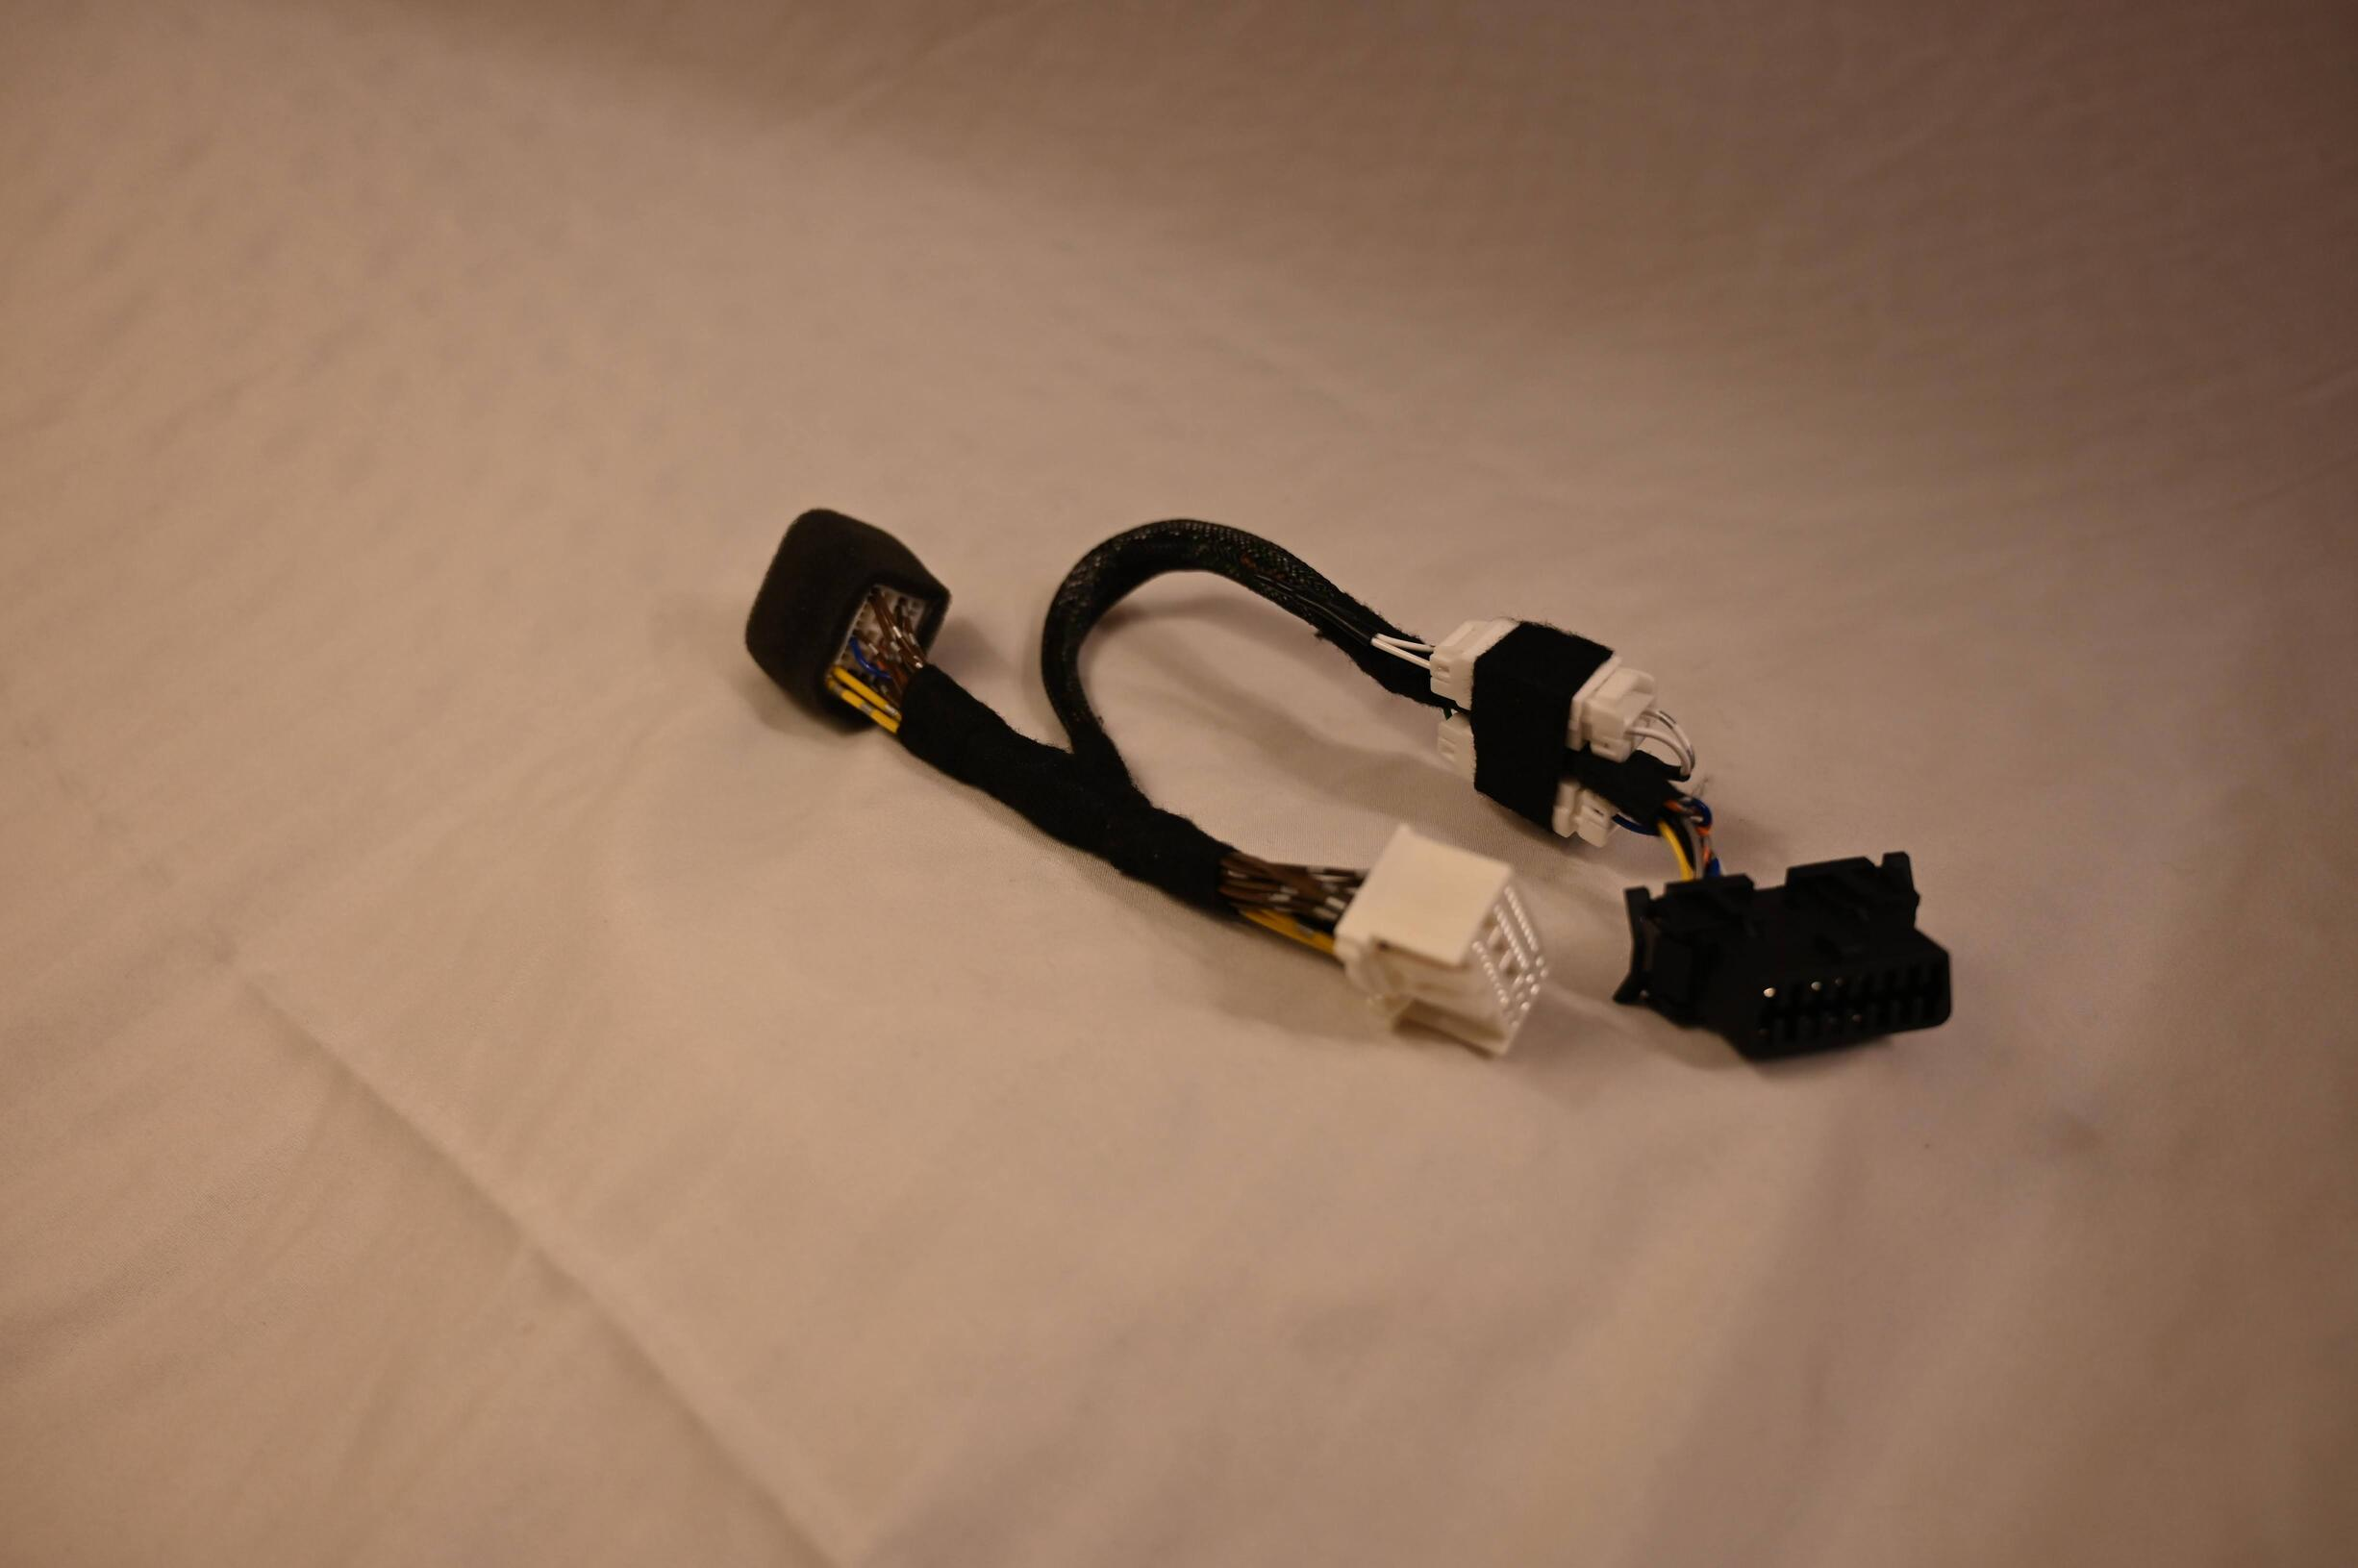
\includegraphics[height=1.95in]{../../../harnesses/head_unit_MITM/photos/whole_harness.jpg} } \\
  \subfloat[]{\label{subfig:overview:trim}
  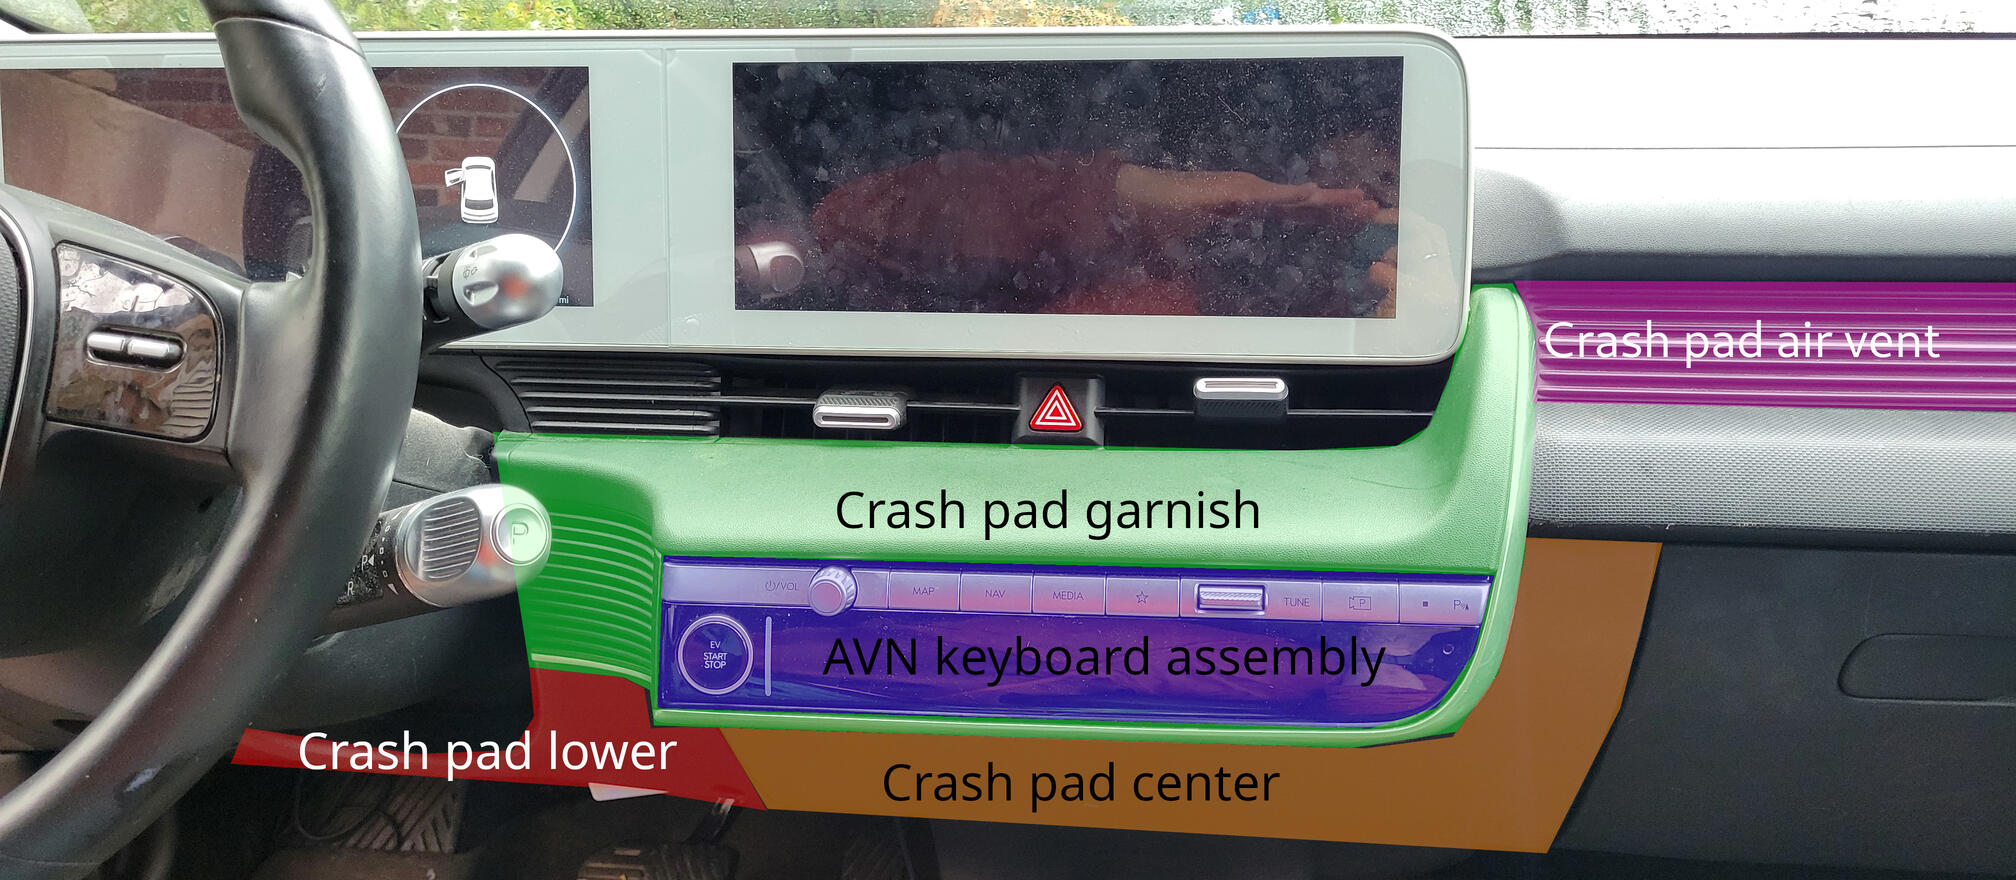
\includegraphics[width=6in]{photos/overview_labeled.jpg} }
   \caption{(a) Harnais d'homme au milieu. (b) Aperçu des panneaux de garniture concernés. \label{fig:overview}}
\end{figure}

\section{Introduction}
  Le but de ce guide est d'illustrer les instructions étape par étape pour l'installation du kit de préconditionnement de l'unité principale, ou simplement du faisceau d'homme au milieu (MITM) de l'unité principale, illustré dans la figure \ref{subfig:overview:harness}. Dans la rubrique \ref{sect:1}, nous présentons deux options de retrait des garnitures pour accéder à l'unité principale. Dans la rubrique \ref{sect:2}, nous décrivons le processus de branchement du harnais. Dans la rubrique \ref{sect:3}, nous montrons la fixation du port OBD et comment brancher le microcontrôleur. 

Outils nécessaires :
\begin{enumerate}
  \item Douille de 10 mm ou clé à molette pour batterie 12 V (non incluse)
  \item Outils de suppression de garniture (inclus si sélectionnés)
  \item Phillips \#2 clés Allen (incluses si sélectionnées) ou similaire
\end{enumerate}

Composants du kit :
\begin{enumerate}
  \item Harnais de l'unité principale
  \item WiCAN
  \item Support de montage OBD de 70 mm
  \item Ruban adhésif double face de 70 mm (deux pièces incluses pour la redondance)
  \item 4 attaches zippées
\end{enumerate}

\section{Étape 1 : Retirez la borne négative 12 V} \label{sect:0}
Tout d’abord, débranchez toujours la batterie 12V avant de retirer les connecteurs électriques ! Le retrait d'un connecteur électrique sous tension pourrait provoquer une décharge et détruire un connecteur ou un calculateur dans votre voiture.

Instructions étape par étape :
\begin{enumerate}
  \item Capot ouvert (Figure \ref{subfig:12V:hood})
  \item Porte-bagages ouvert 
  \item Retirez le panneau couvrant 12 V (Figure \ref{subfig:12V:panel})
  \item Desserrez l'écrou du côté négatif avec une douille de 10 mm (Figure \ref{subfig:12V:nut})
  \item Retirez la borne négative (Figure \ref{subfig:12V:terminal})
\end{enumerate}

\begin{figure}[h]
  \subfloat[]{\label{subfig:12V:hood}
  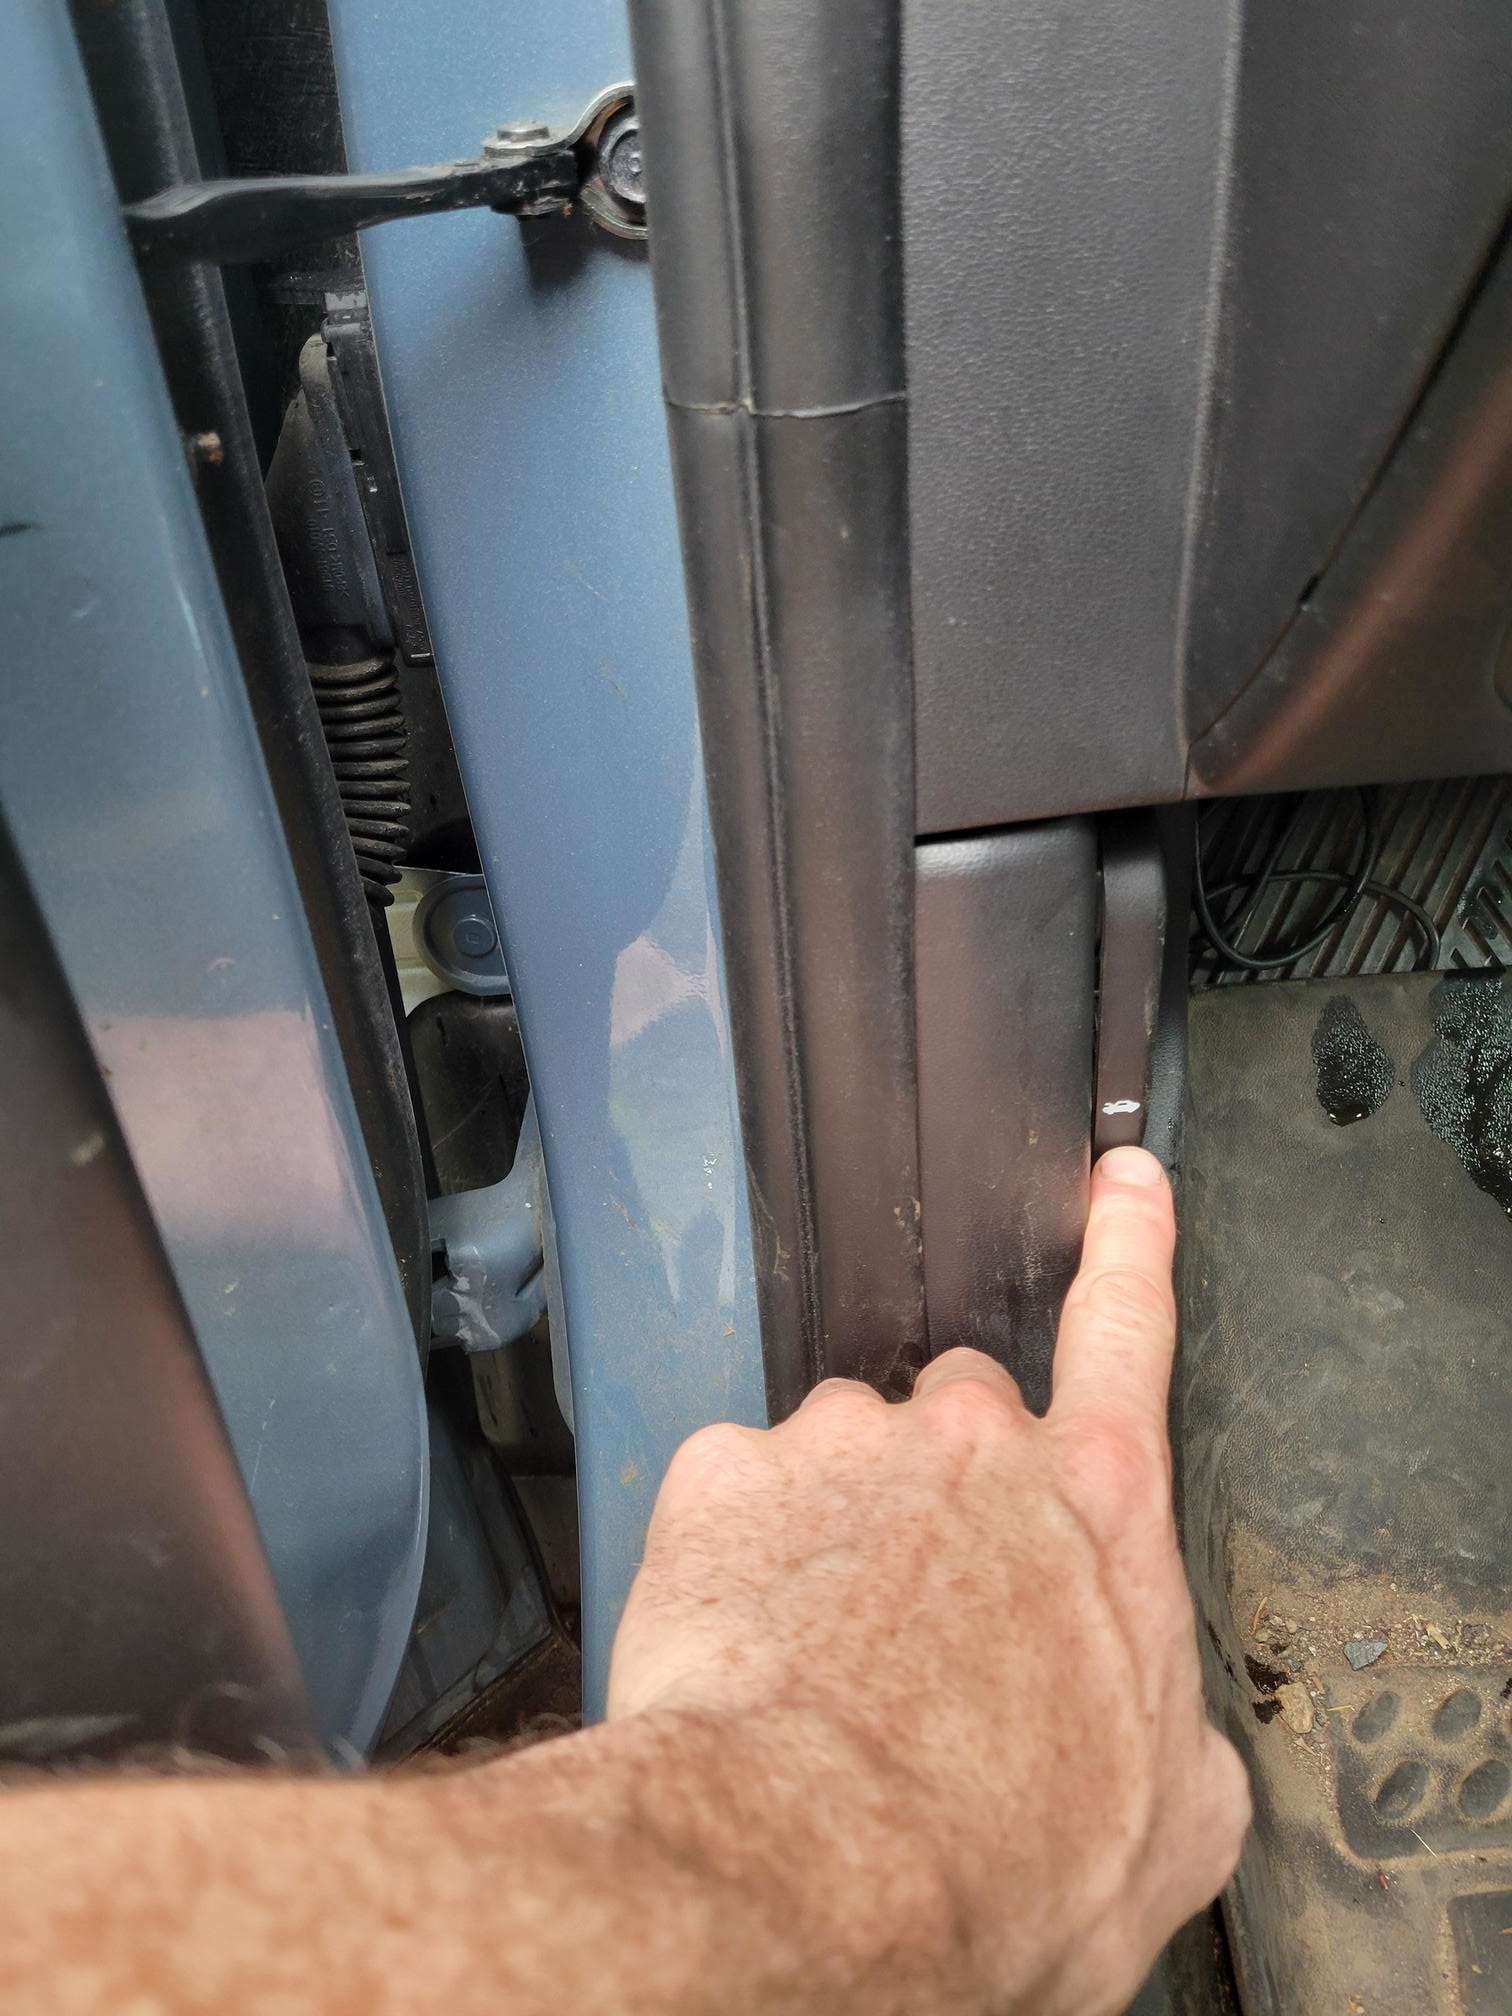
\includegraphics[height=1.5in]{photos/open_hood.jpg} } 
  \subfloat[]{\label{subfig:12V:panel}
  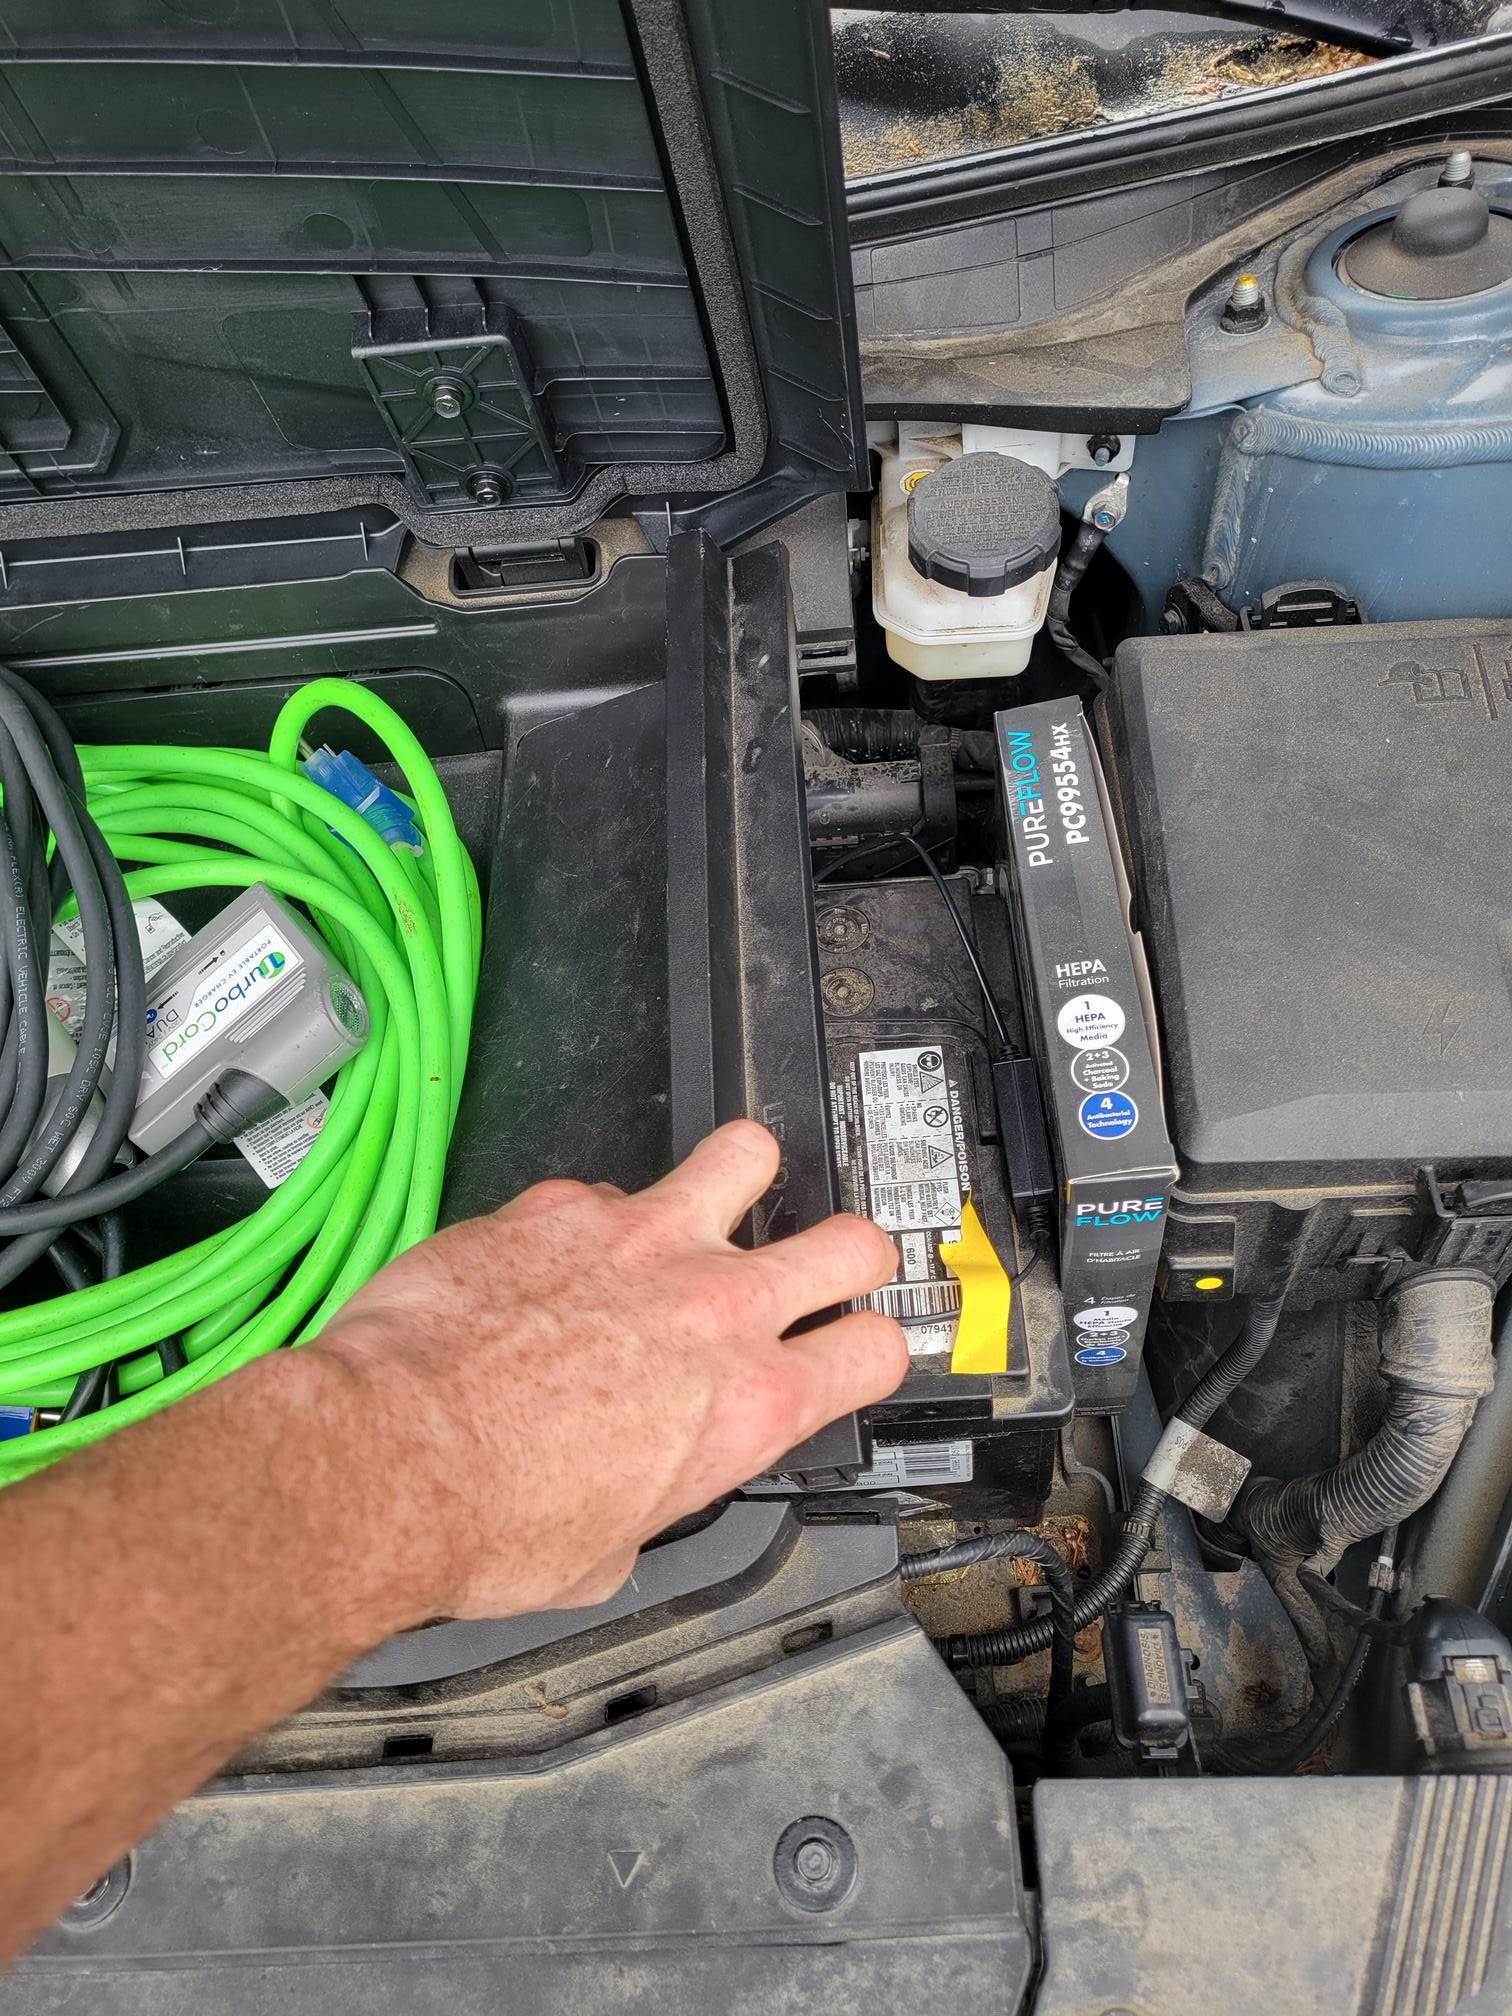
\includegraphics[height=1.5in]{photos/remove_panel.jpg} }  \\
  \subfloat[]{\label{subfig:12V:nut}
  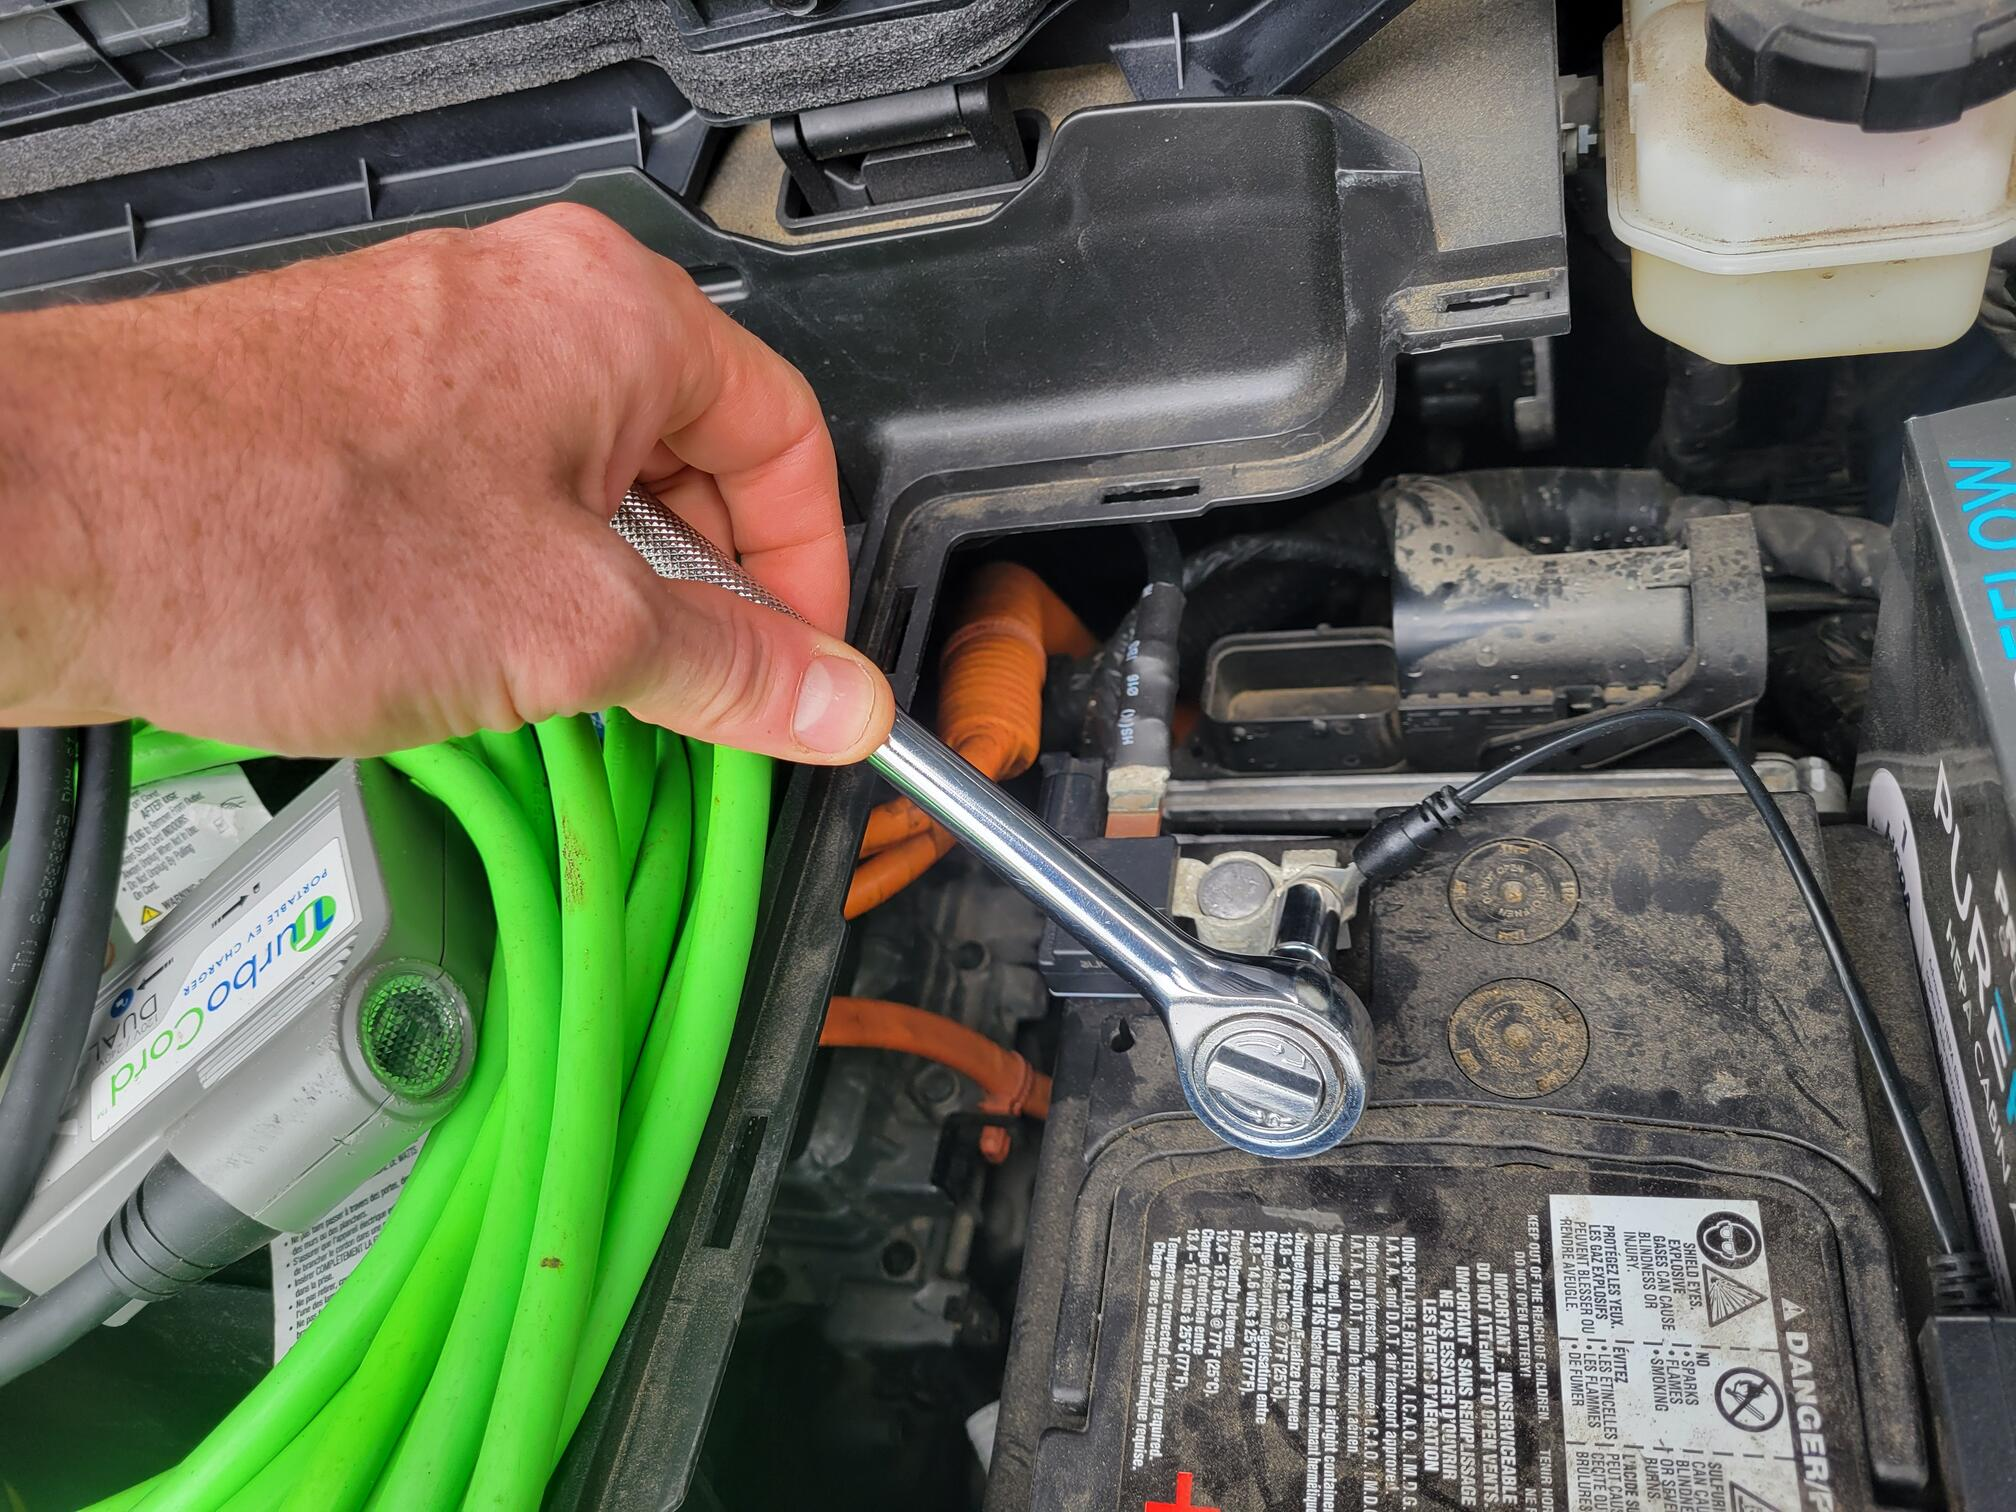
\includegraphics[height=1.5in]{photos/loosen_nut.jpg} } 
  \subfloat[]{\label{subfig:12V:terminal}
  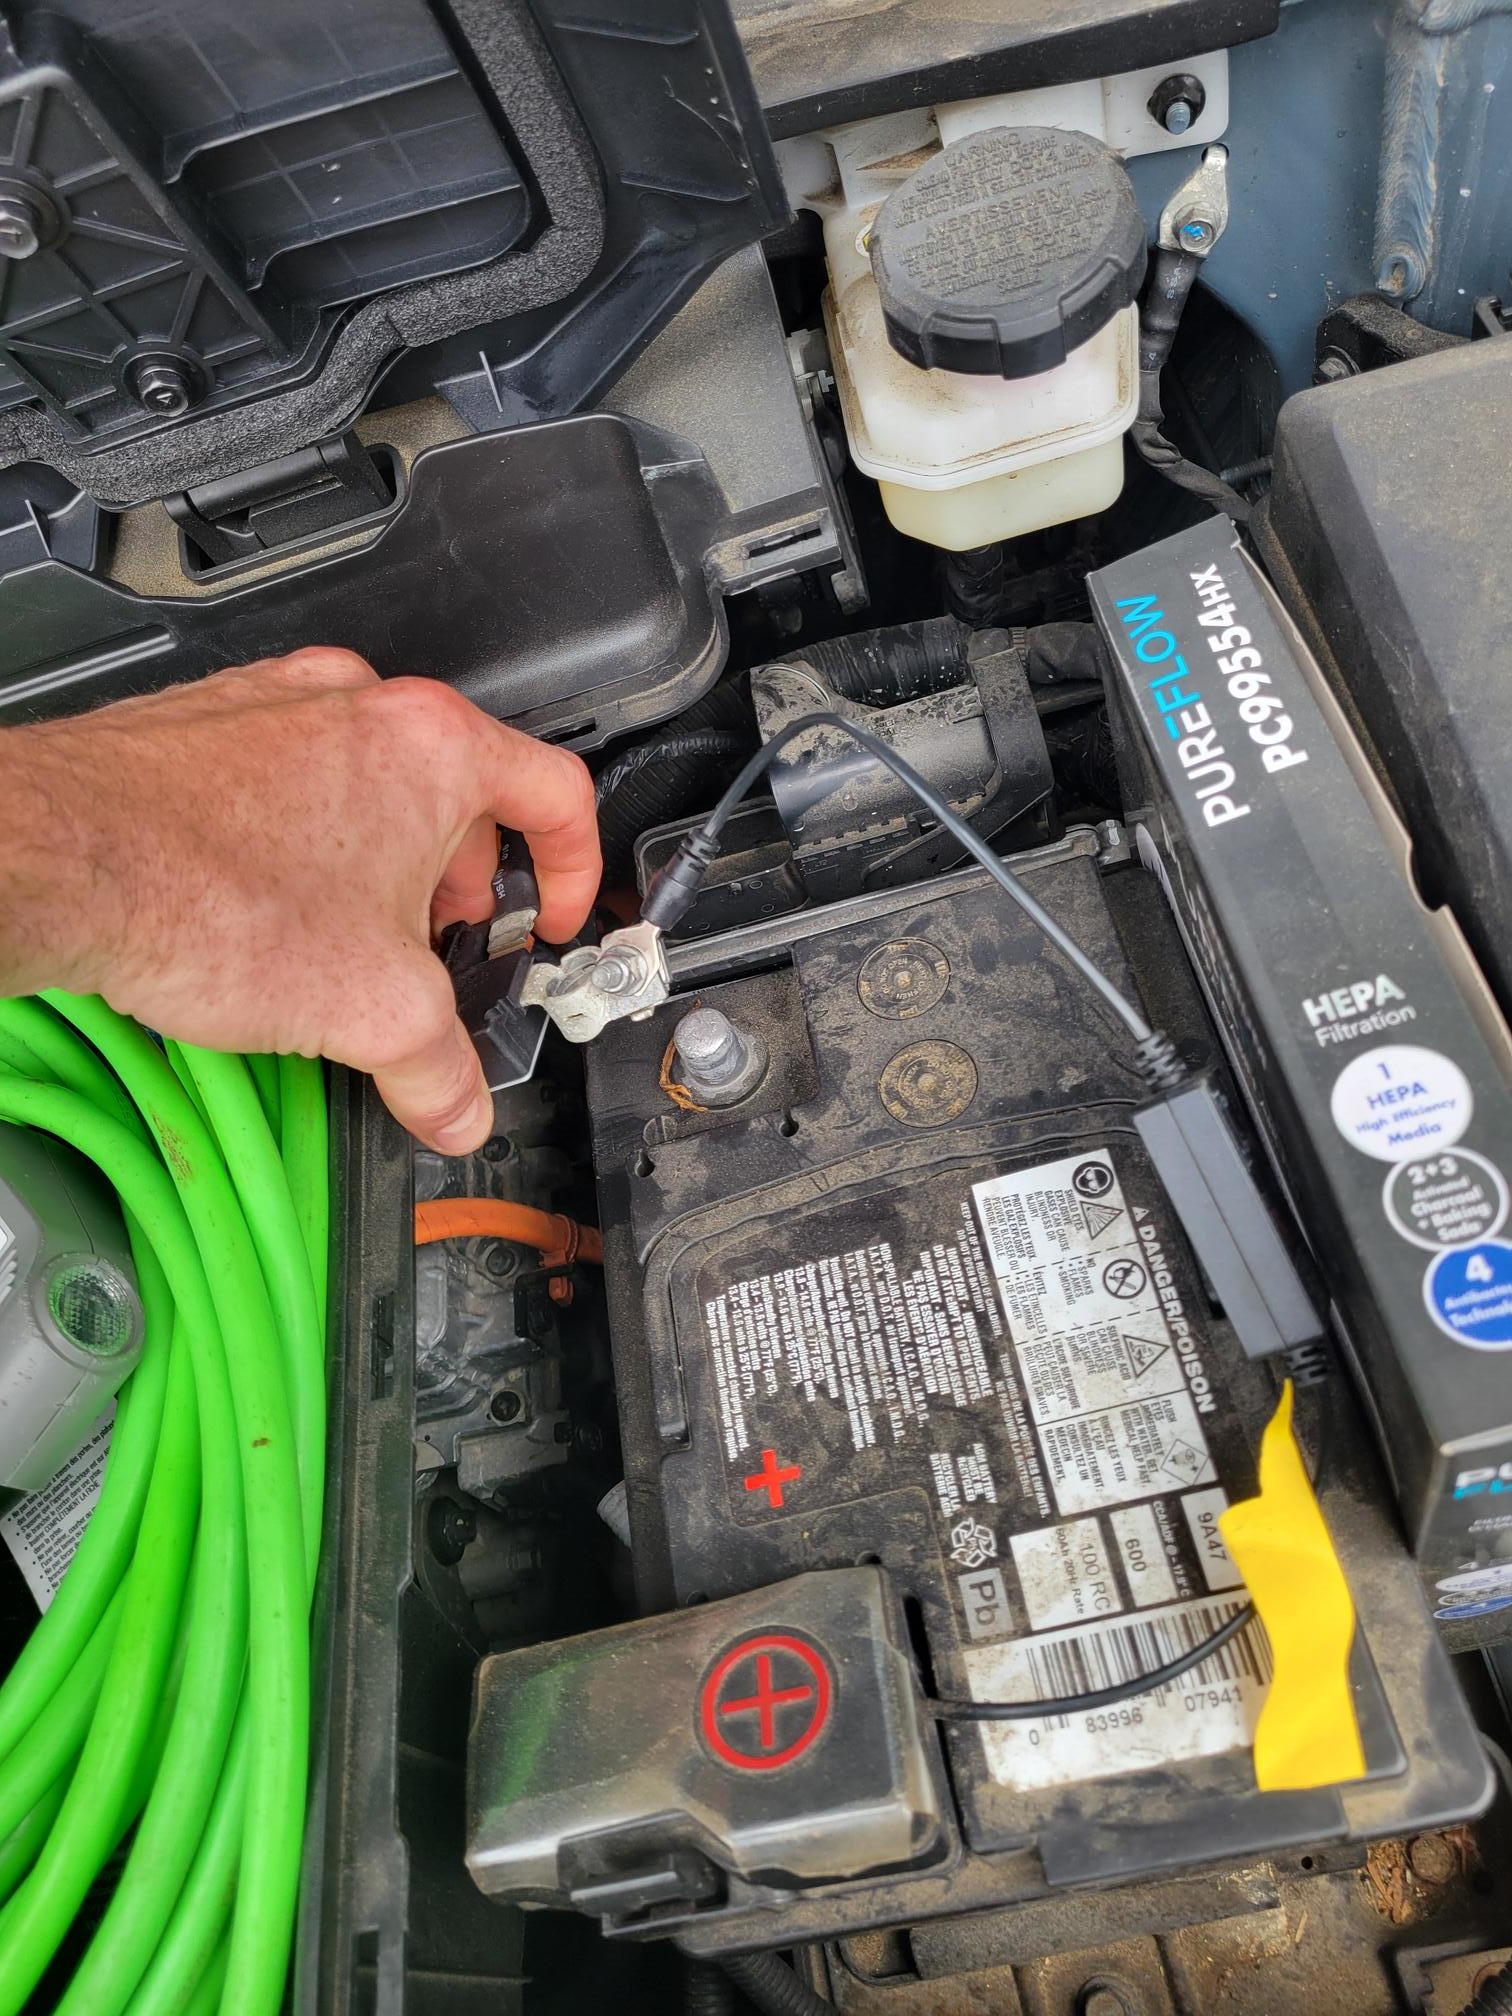
\includegraphics[height=1.5in]{photos/disconnect_terminal.jpg} } 
   \caption{(a) Ouvrez le capot. (b) Retirez le panneau recouvrant 12 V. (c) Desserrez l'écrou sur la borne négative. (d) Retirez la borne négative. \label{fig:12V}}
\end{figure}

\section{Étape 2 : Couper} \label{sect:1}
Le but ici est d'accéder au coffre au trésor : l'unité principale. La bonne méthode consiste à retirer 4 pièces de garniture et le clavier AVN (barre de boutons climatiques). Il est également possible de prendre un raccourci. Le raccourci est beaucoup plus rapide mais plus délicat, avec un risque plus élevé de se coincer la main sur un bord tranchant. Choisissez la méthode qui vous convient le mieux.
\begin{figure}[h]
  \subfloat[]{\label{subfig:step1:X}
  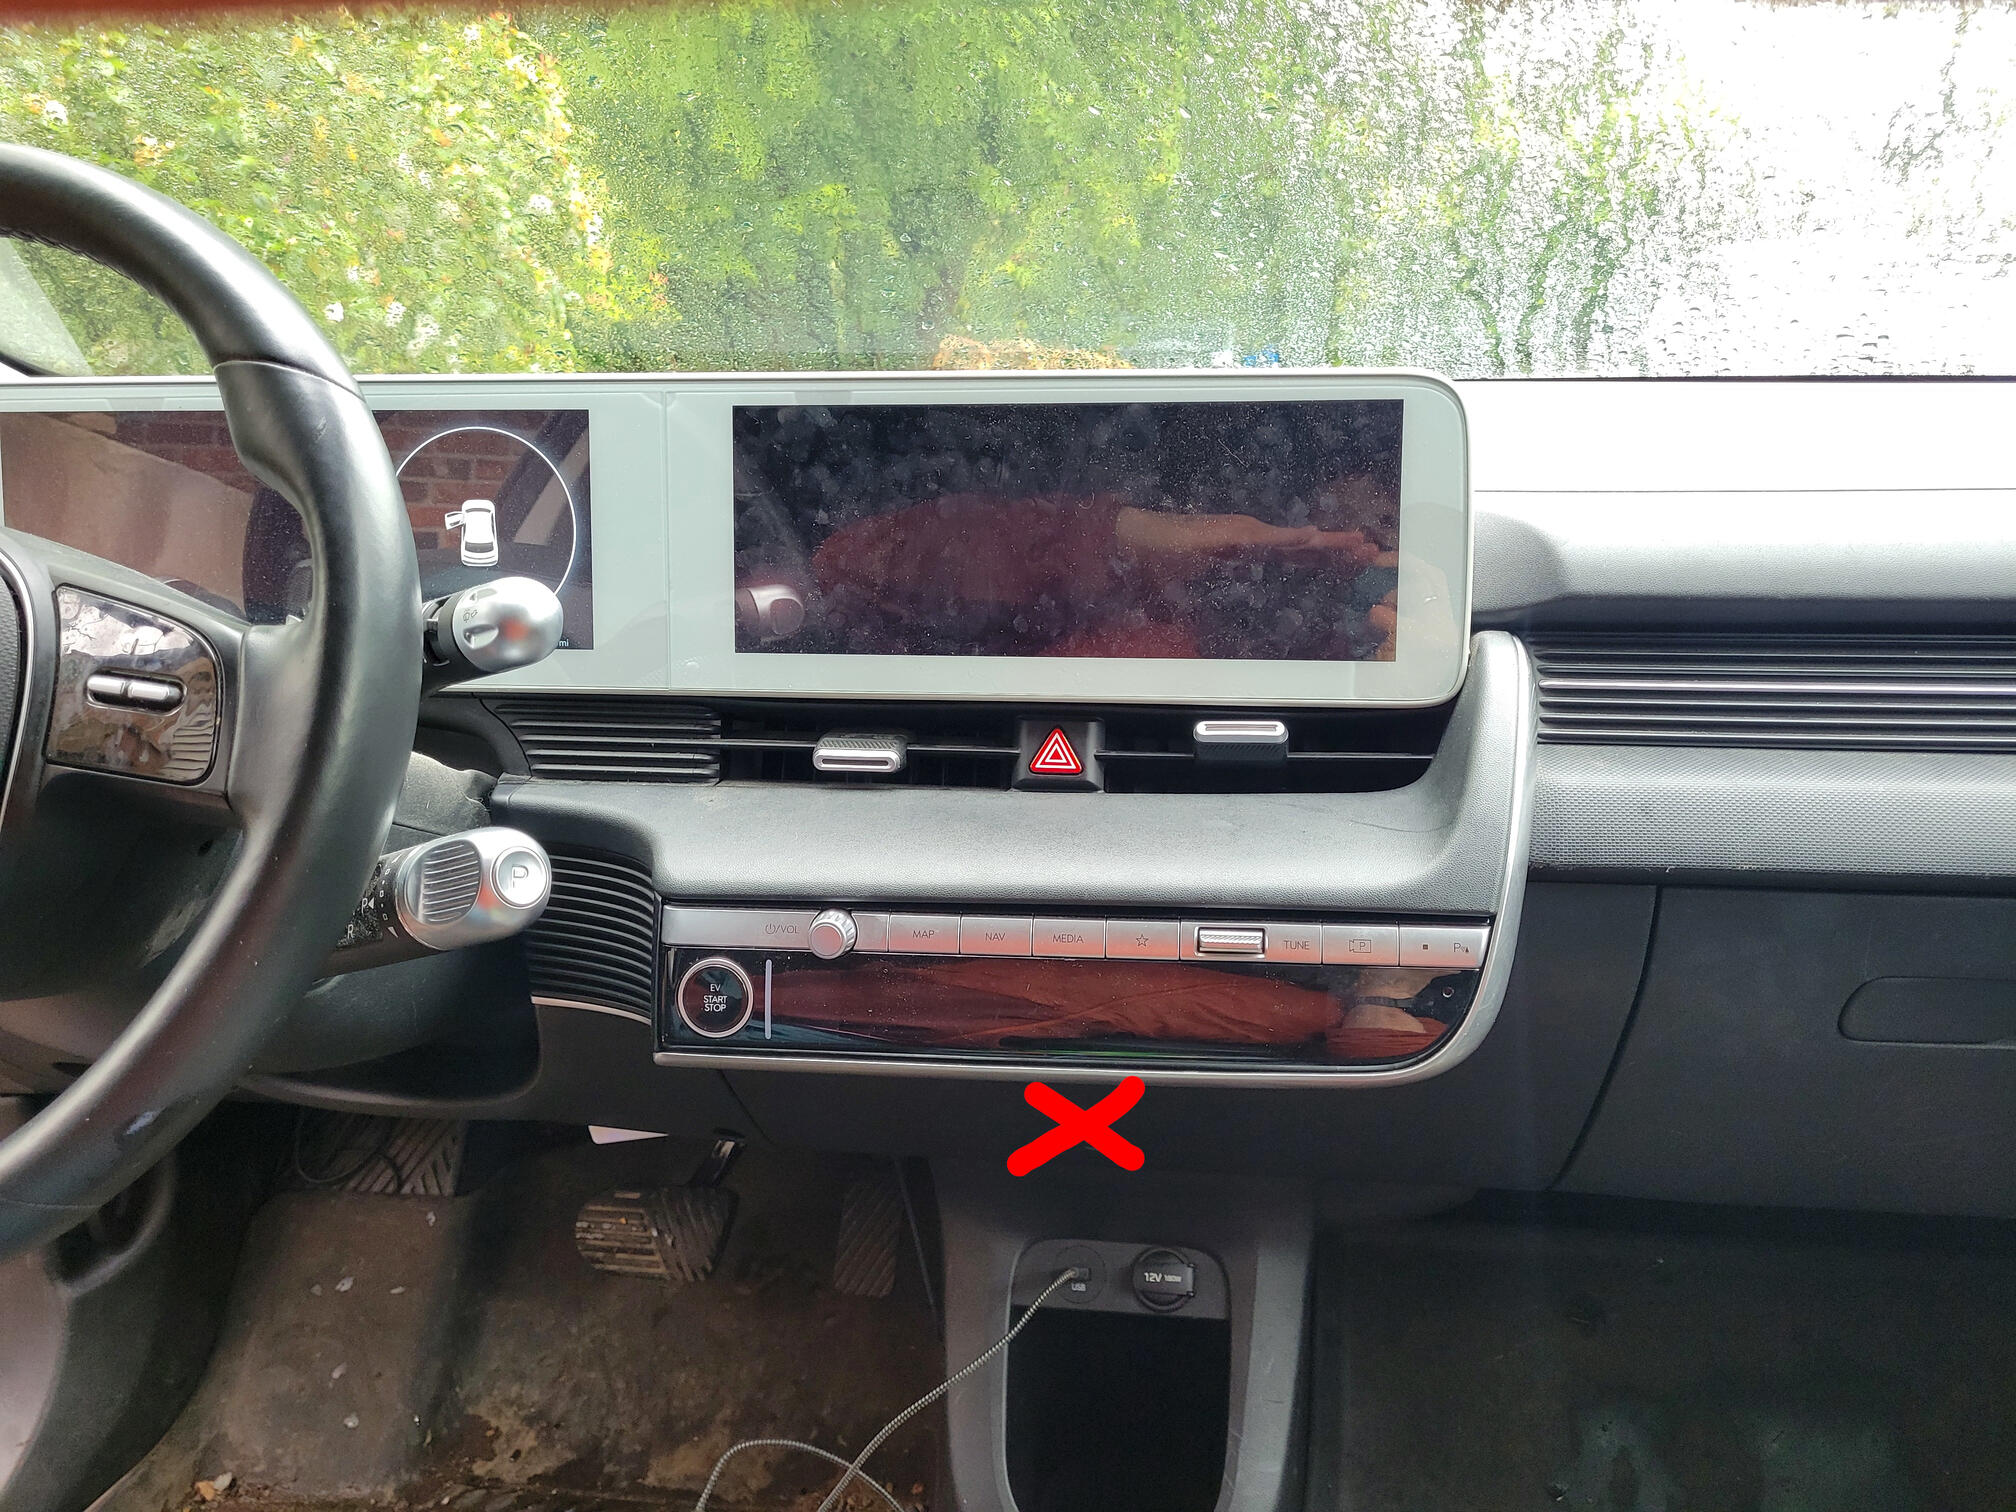
\includegraphics[height=2.95in]{photos/overview_X.jpg} } 
   \caption{X marque l'unité principale. \label{fig:step1}}
\end{figure}

\begin{figure}[h]
  \subfloat[]{\label{subfig:trim:lower}
  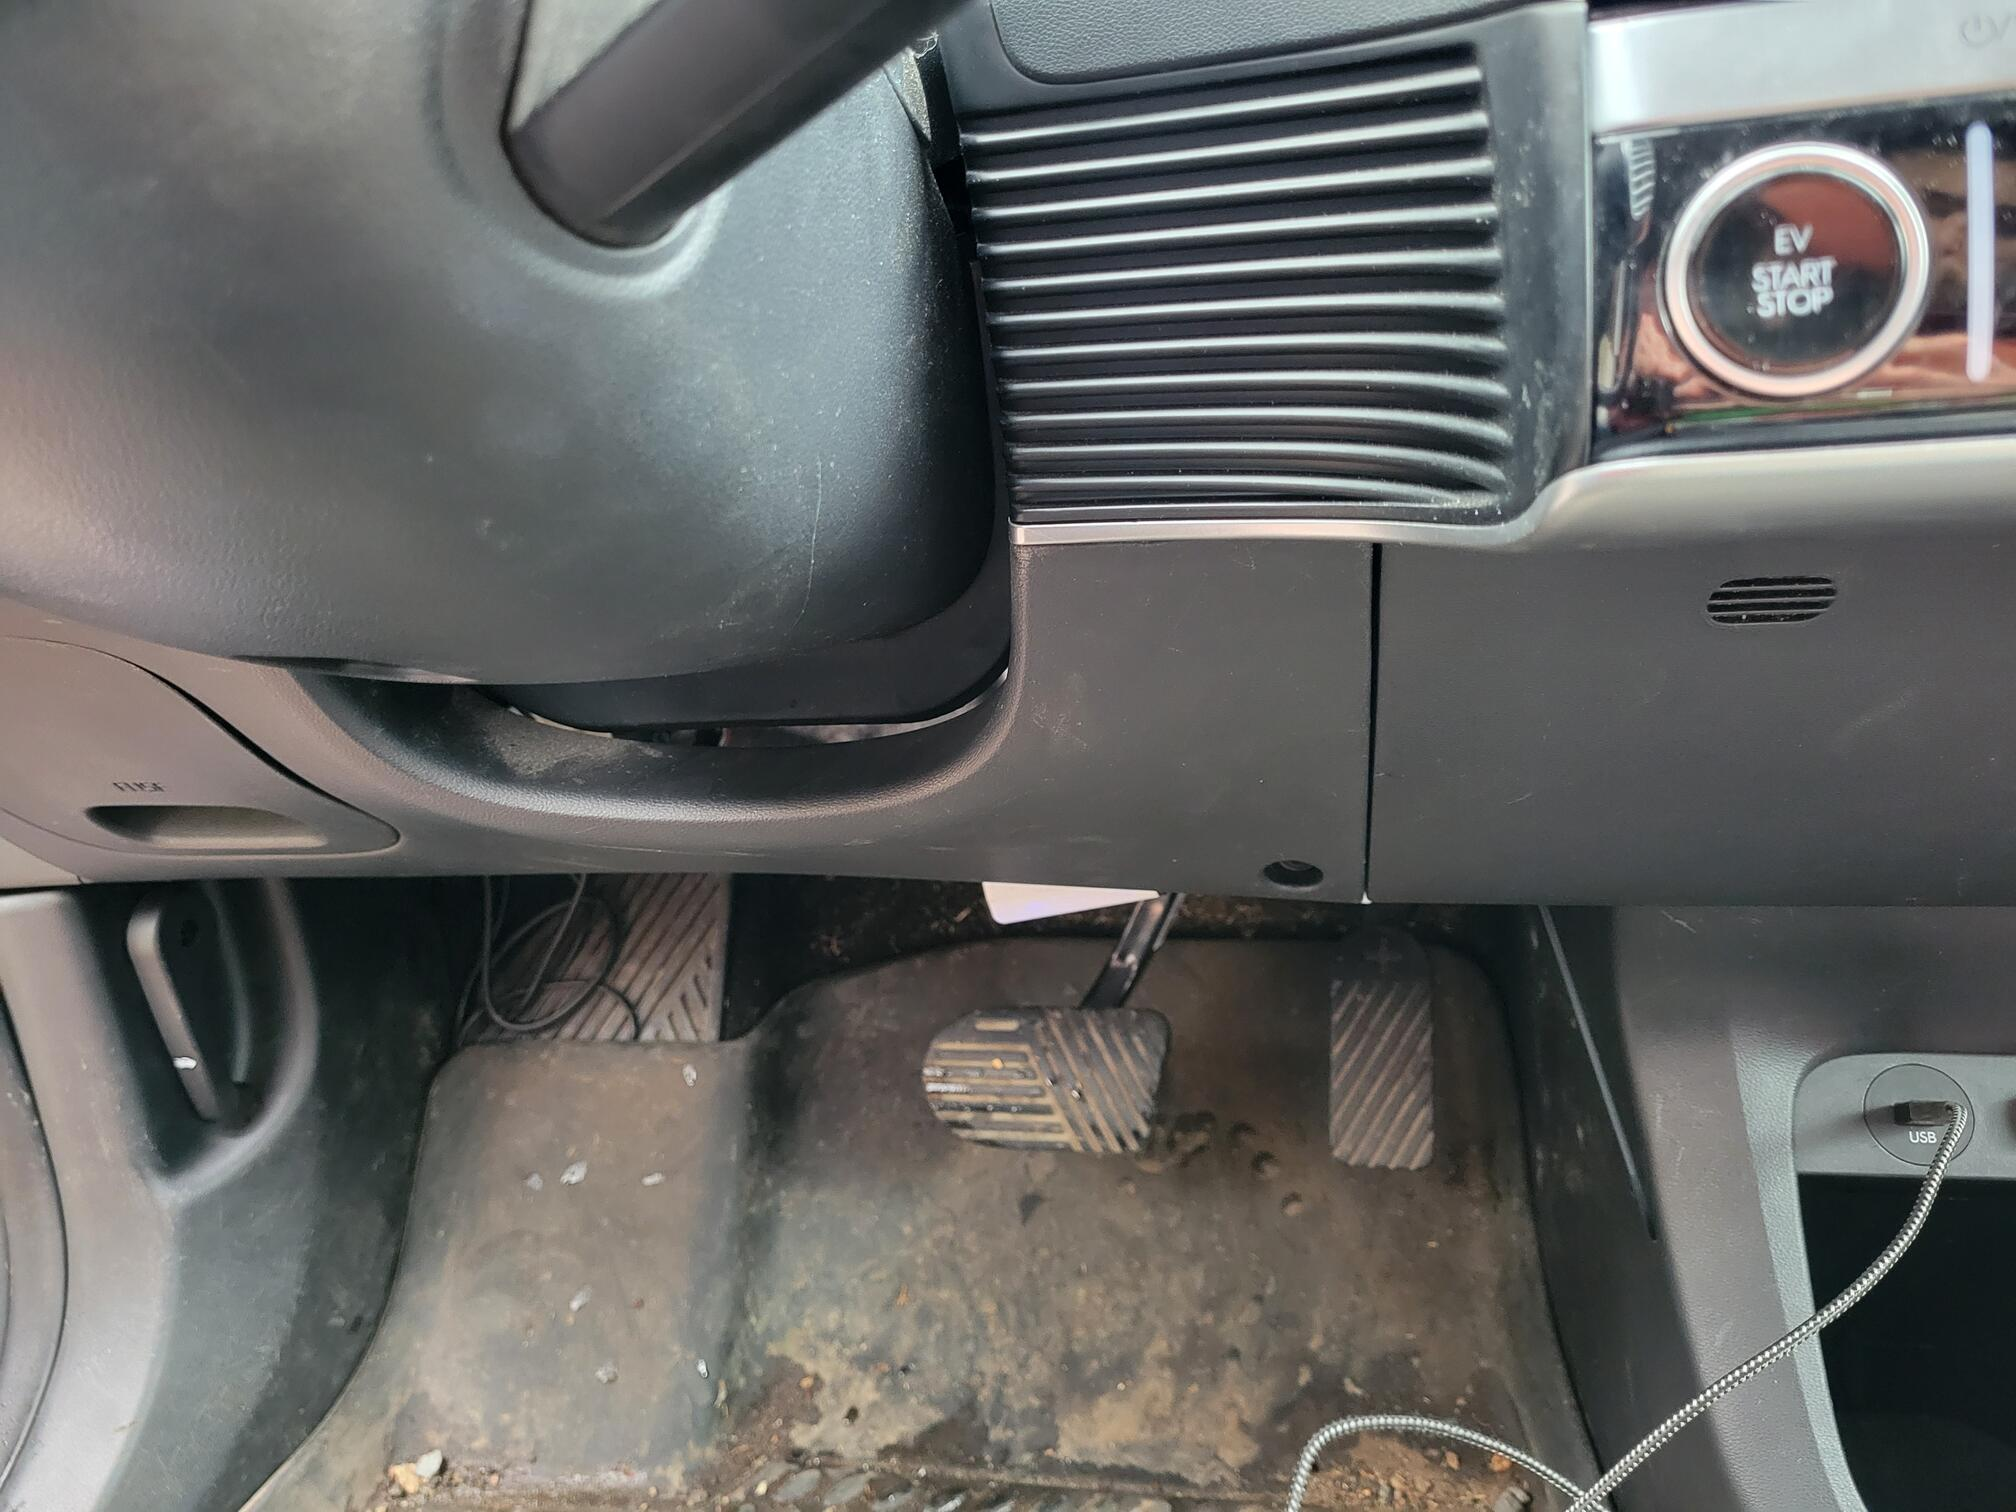
\includegraphics[height=1.5in]{photos/crash_pad_lower.jpg} } 
  \subfloat[]{\label{subfig:trim:airvent}
  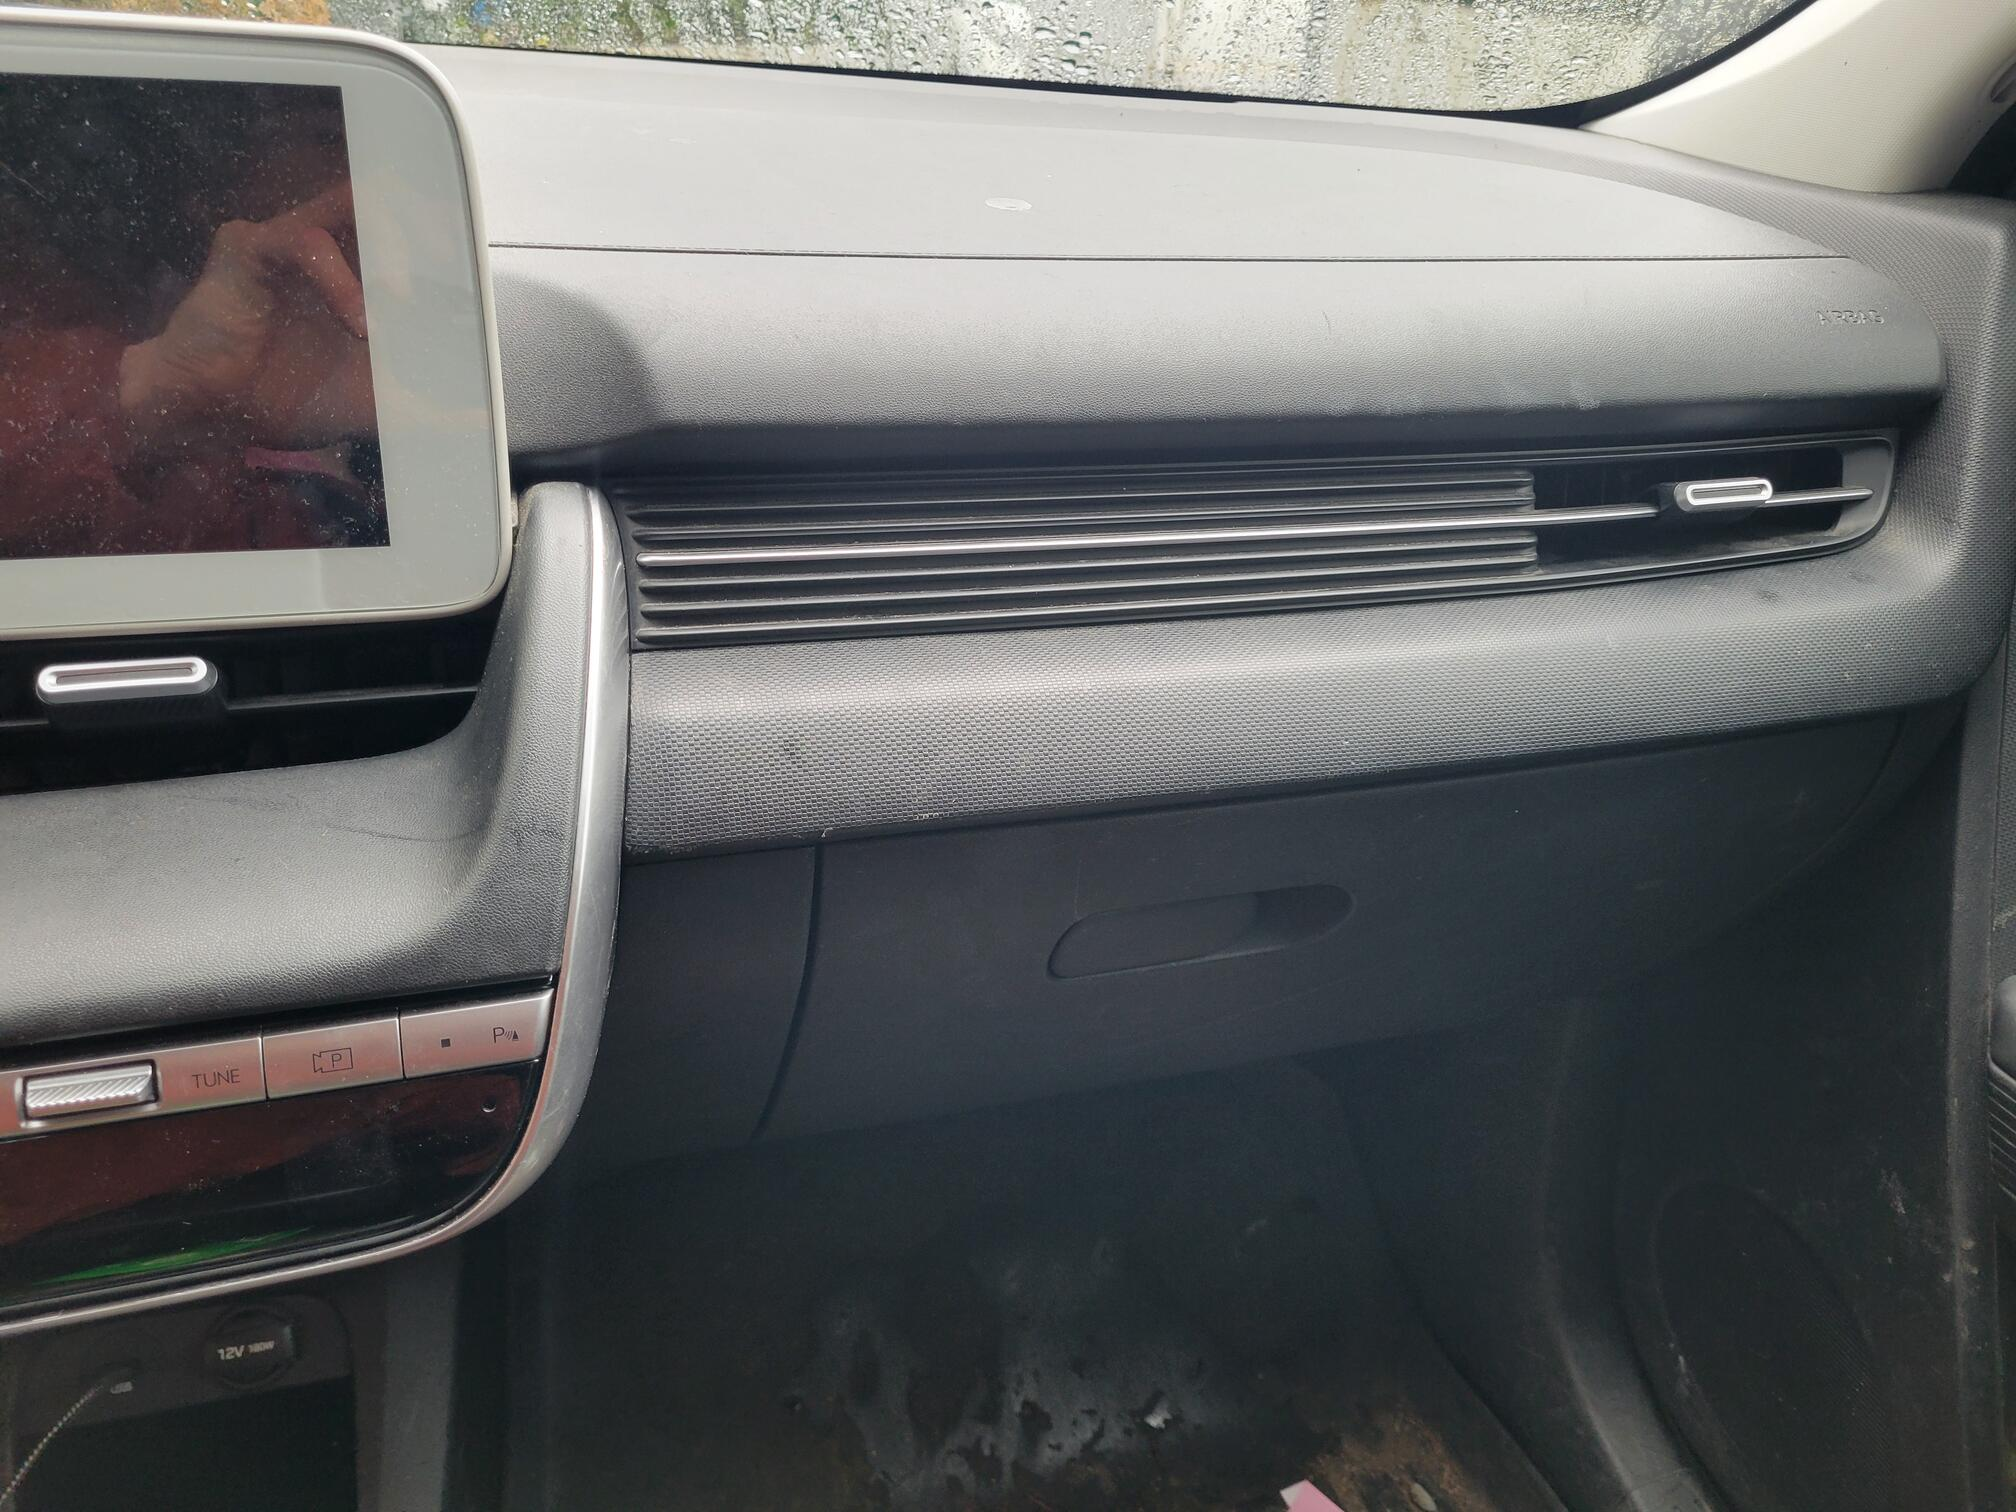
\includegraphics[height=1.5in]{photos/crash_pad_air_vent.jpg} } 
  \subfloat[]{\label{subfig:trim:center}
  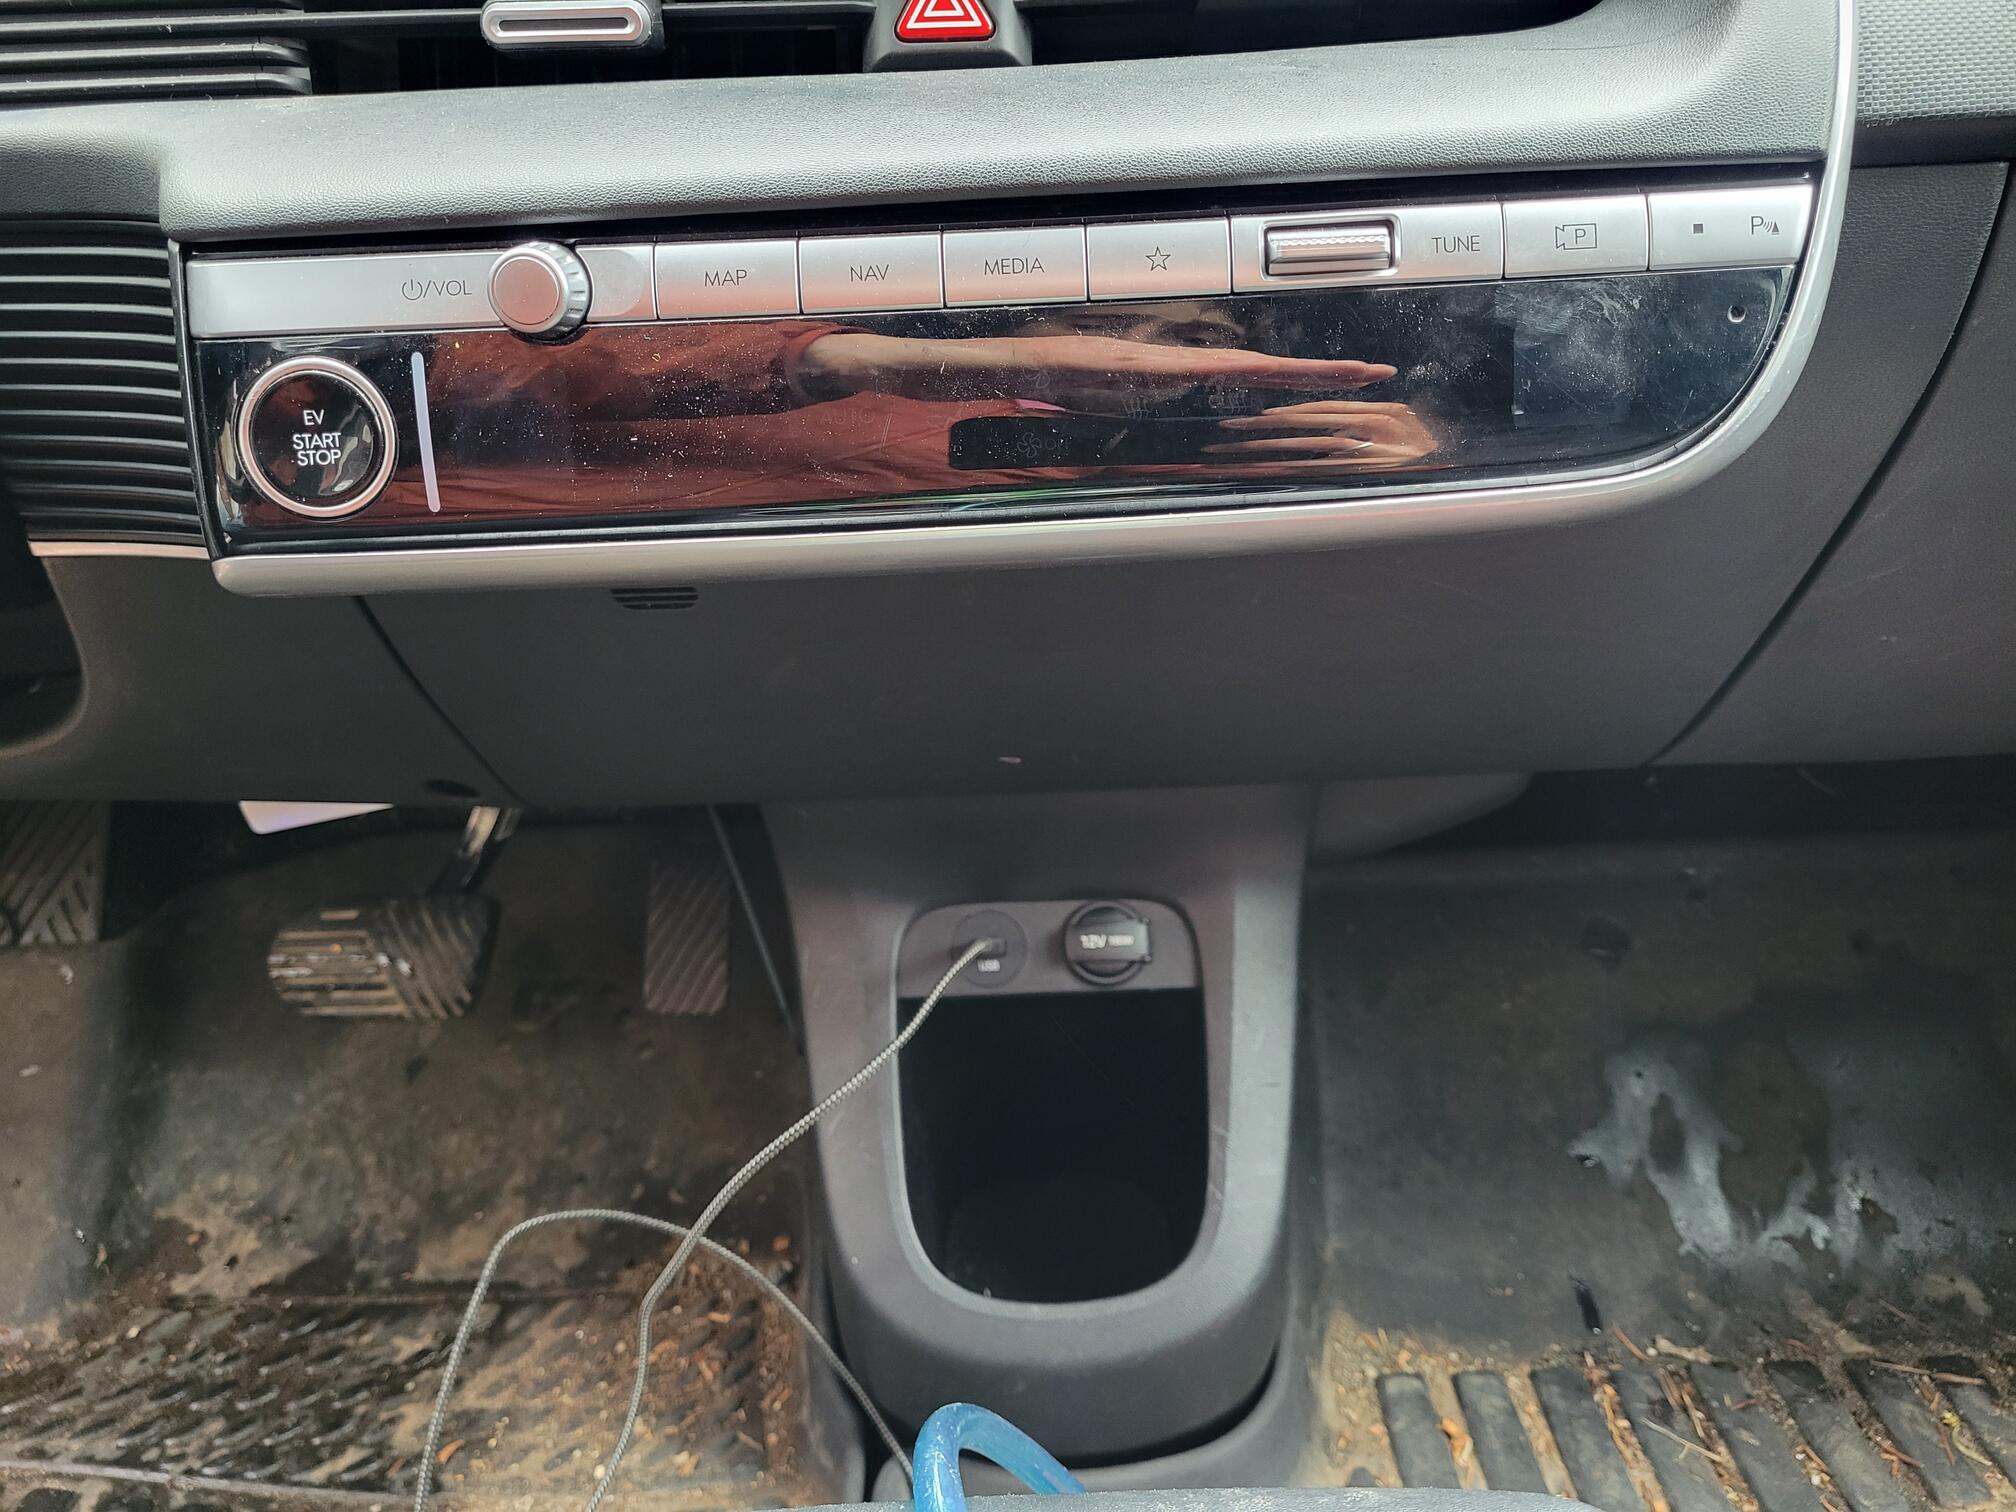
\includegraphics[height=1.5in]{photos/crash_pad_center_and_keyboard.jpg} } 
   \caption{(a) Patin de protection inférieur. (b) Bouche d'aération du coussin de protection. (c) Garniture du crash pad, clavier AVN et centre du crash pad. \label{fig:trim}}
\end{figure}

\subsection{Option A : longue et prudente}
Ordre des opérations du panneau de garniture : 
\begin{enumerate}
  \item Patin de protection inférieur (Figure \ref{subfig:trim:lower}) \label{step:cpl}
  \item Grille d'aération du coussin de protection (Figure \ref{subfig:trim:airvent}) \label{step:cpav}
  \item Garniture de protection de protection (Figure \ref{subfig:trim:center})
  \item Clavier AVN (figure \ref{subfig:trim:center})
  \item Centre du coussin de protection (Figure \ref{subfig:trim:center})
\end{enumerate}

Mesures \ref{step:cpl} et \ref{step:cpav} peut être fait dans n’importe quel ordre ; les deux doivent être effectués pour libérer la garniture du crash pad.

Instructions étape par étape :
\begin{enumerate}
  \item Retirez la vis du crash pad inférieur (Figure \ref{subfig:trimsteps:lowerscrew})
  \item Retirez la moitié droite du crash pad inférieur à l'aide des outils de dépose de garniture.
  \item Pendant que vous êtes ici, retirez la ou les vis derrière le crash pad inférieur (il peut y en avoir 1 ou 2 ; voir la figure \ref{subfig:trimsteps:cpc_llscrews}); la vis la plus à gauche fixée à l'évent derrière a tendance à rester captive, vous devez donc tirer pour confirmer qu'elle est retirée (Figure \ref{subfig:trimsteps:cpc_llscrew})
  \item Retirer l'évent du crash pad
  \item Retirez la vis qui était cachée derrière la grille d'aération du crash pad (Figure \ref{subfig:trimsteps:cpg_r_screw})
  \item Retirer la garniture du crash pad
  \item Détacher le clavier AVN 
    \begin{enumerate}
      \item Retirez la vis gauche (Figure \ref{subfig:trimsteps:keyboard_l_screw})
      \item Retirez la vis droite (Figure \ref{subfig:trimsteps:keyboard_ur_screw})
      \item Retirez la vis inférieure gauche (Figure \ref{subfig:trimsteps:keyboard_ll_screw})
      \item Retirez la vis inférieure droite (Figure \ref{subfig:trimsteps:keyboard_lr_screw})
      \item (facultatif, vérifiez l'absence d'alimentation 12 V) Retirez tous les connecteurs électriques à l'arrière du clavier AVN.
      \item Déconnectez les clips de garniture en tirant vers l'extérieur sur le clavier (Figure \ref{subfig:trimsteps:remove_keyboard})
      \item Si les connecteurs électriques sont toujours connectés, évitez de mettre trop de tension dessus
    \end{enumerate}
  \item Retirez la vis supérieure droite centrale du crash pad qui était bloquée par le clavier AVN (Figure \ref{subfig:trimsteps:cpc_urscrew})
  \item (facultatif) Réinsérez le clavier AVN pour le conserver en toute sécurité si les connecteurs électriques sont toujours connectés
  \item Retirez la vis supérieure gauche centrale du crash pad (Figure \ref{subfig:trimsteps:cpc_ulscrew})
  \item Retirez le panneau de garniture central du crash pad à l'aide des outils de dépose de garniture.
  \item (vérifiez d'abord l'absence d'alimentation 12 V) Débranchez le connecteur électrique de l'arrière du panneau et éloignez-le de la zone de travail.
\end{enumerate}

\begin{figure}[h]
  \subfloat[]{\label{subfig:trimsteps:lowerscrew}
  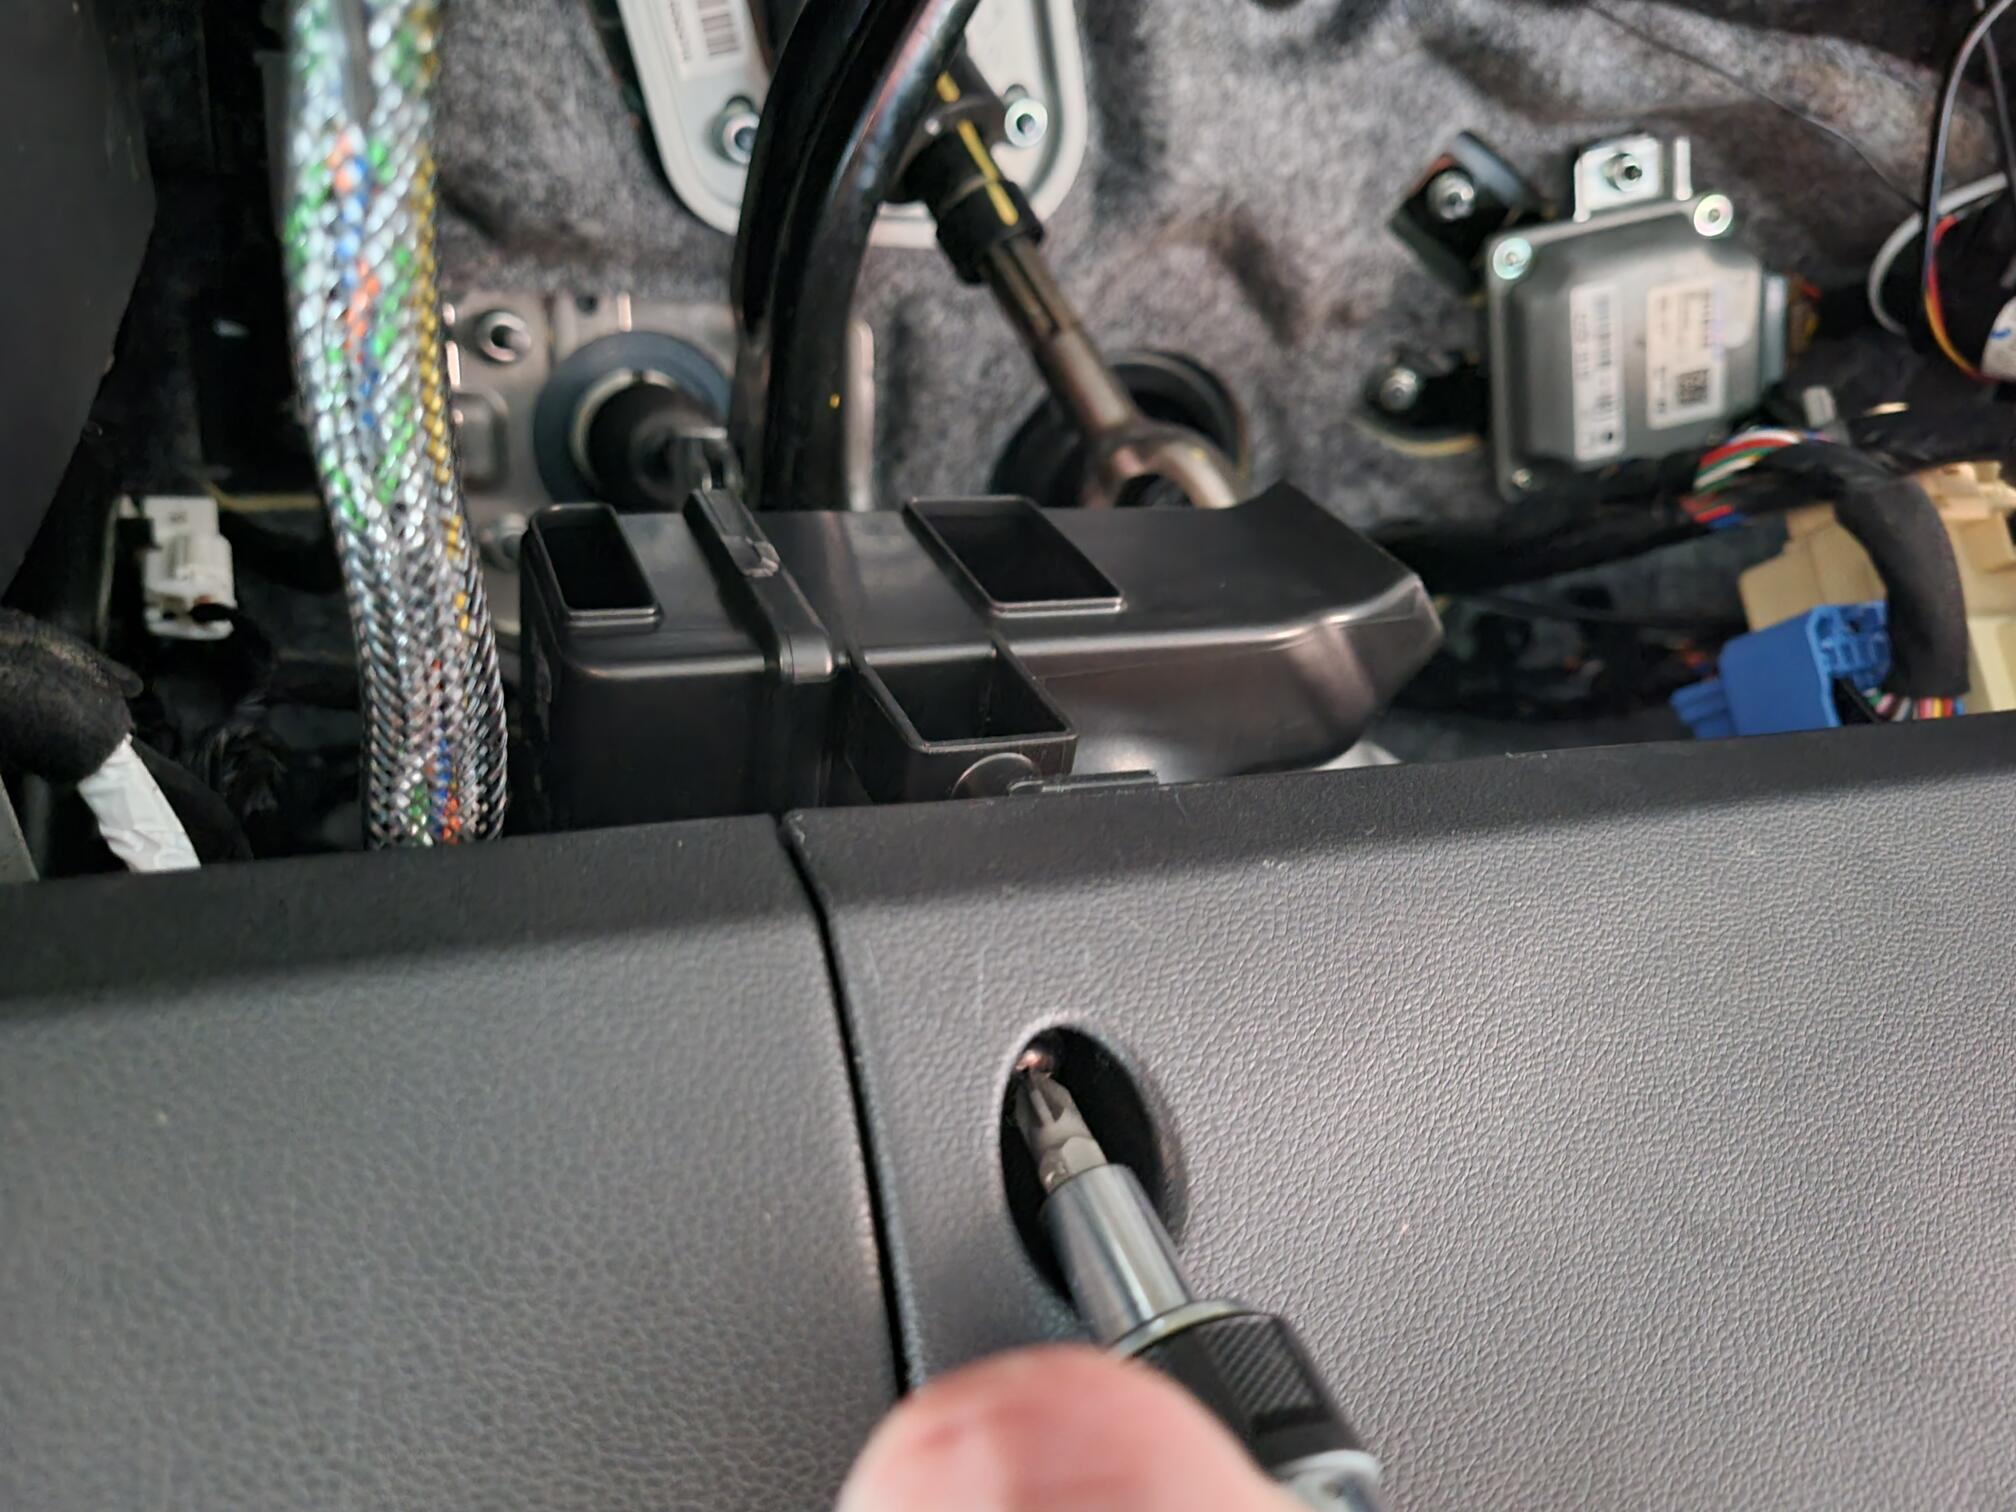
\includegraphics[height=1.5in,angle=180]{photos/crash_pad_lower_screw.jpg} } 
  \subfloat[]{\label{subfig:trimsteps:cpc_llscrews}
  \includegraphics[height=1.5in,angle=180]{photos/crash_pad_center_ll_screws_3.jpg} } 
  \subfloat[]{\label{subfig:trimsteps:cpc_llscrew}
  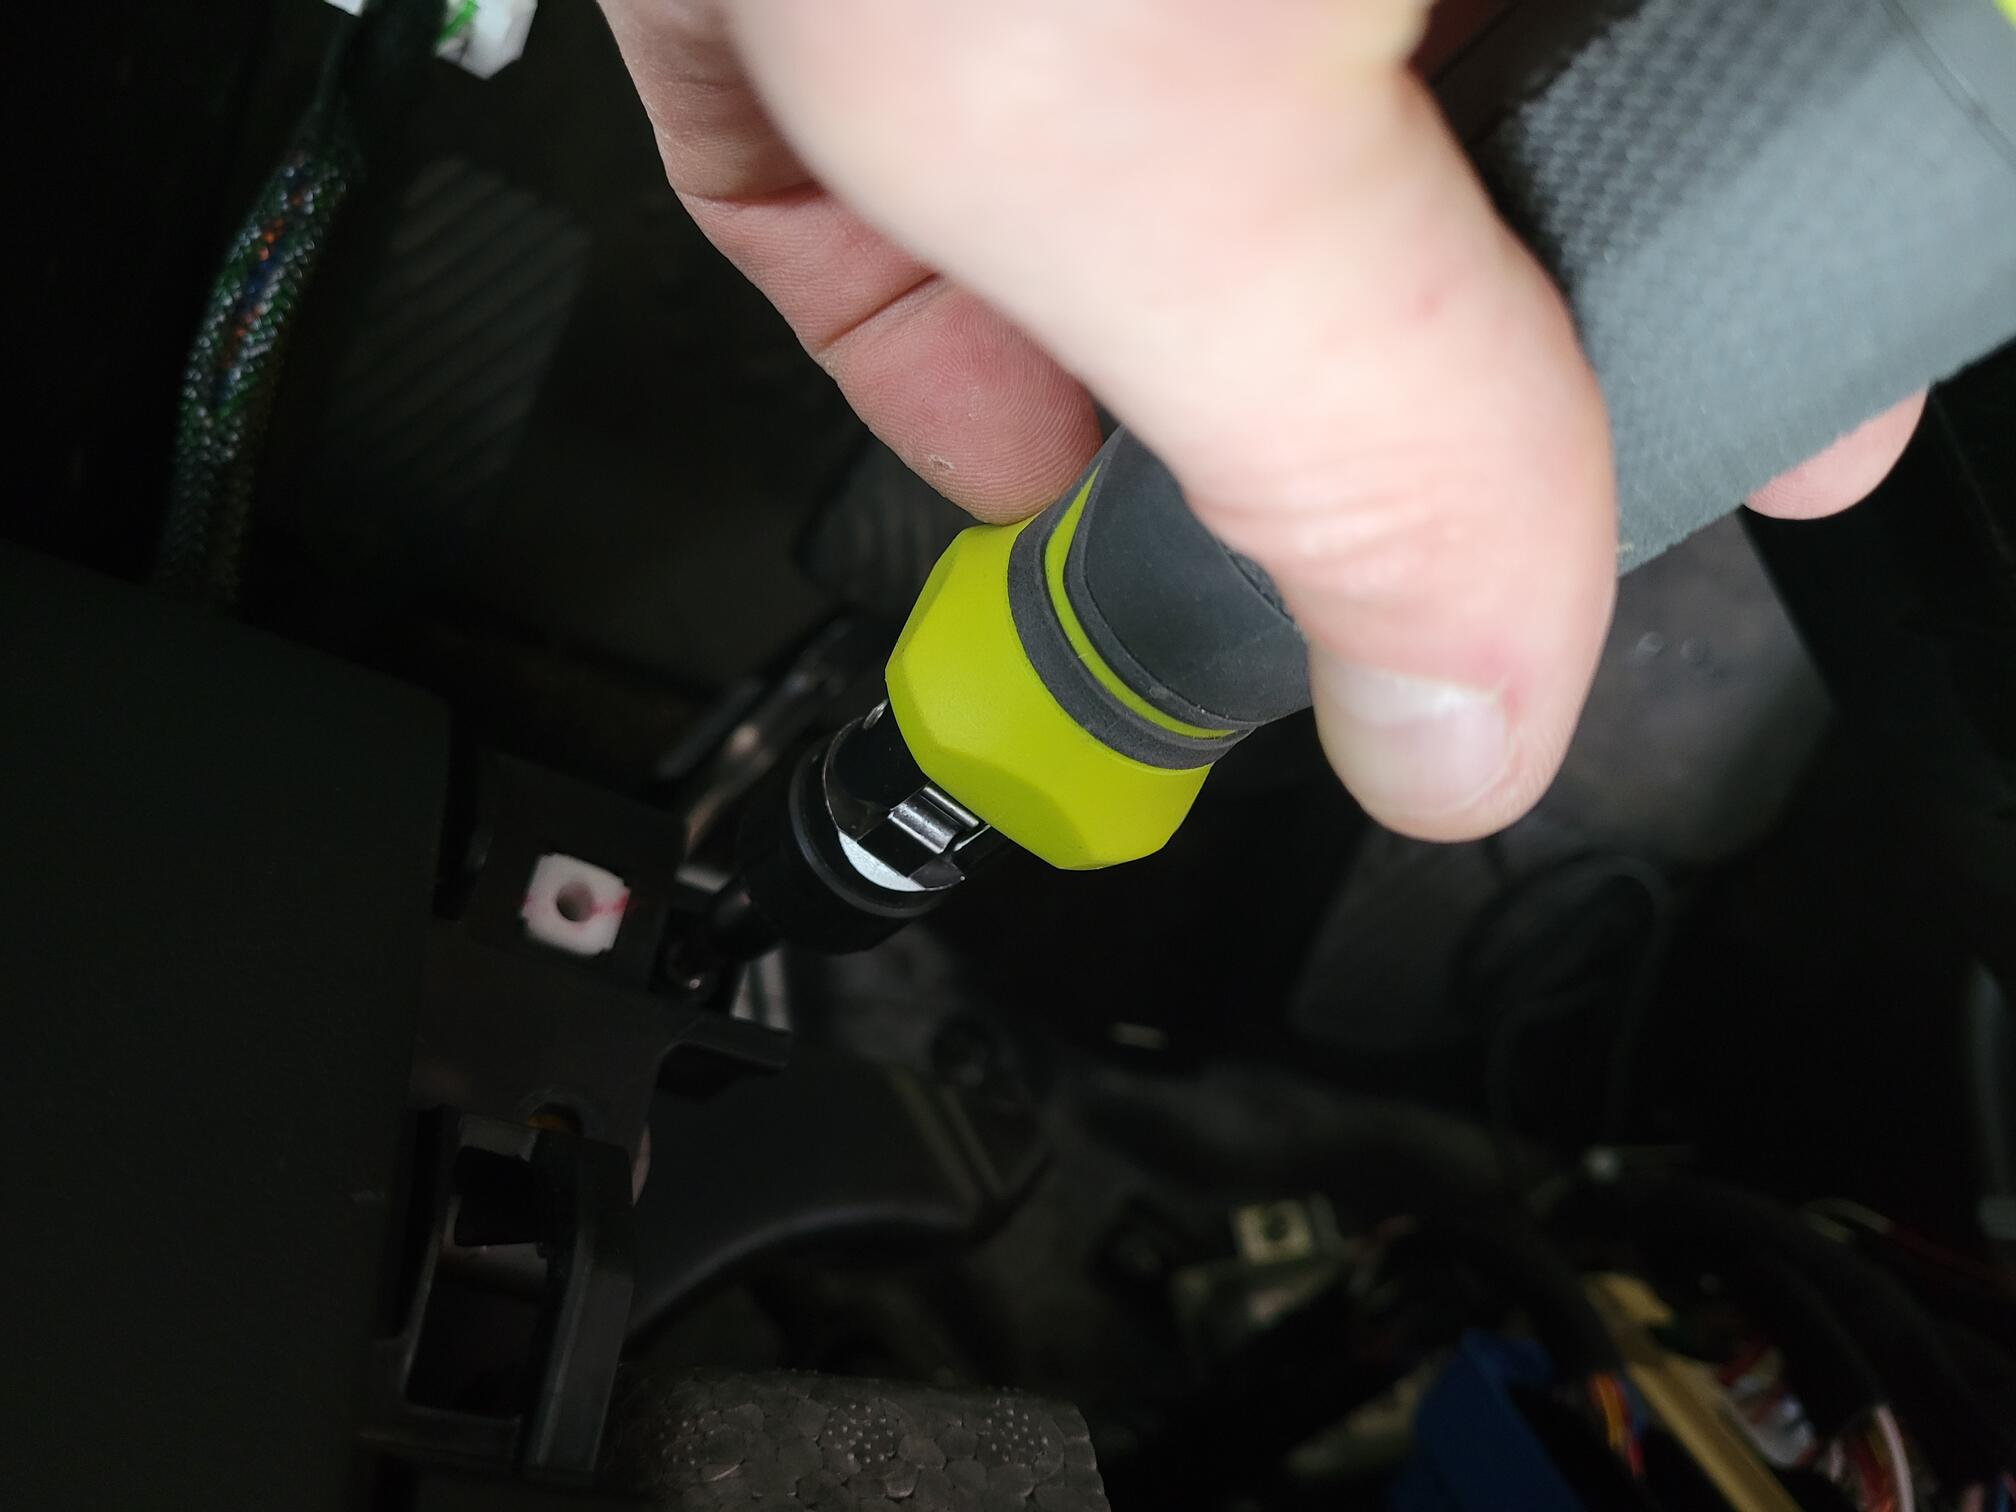
\includegraphics[height=1.5in,angle=180]{photos/crash_pad_center_ll_screw.jpg} } 
  \subfloat[]{\label{subfig:trimsteps:cpg_r_screw}
  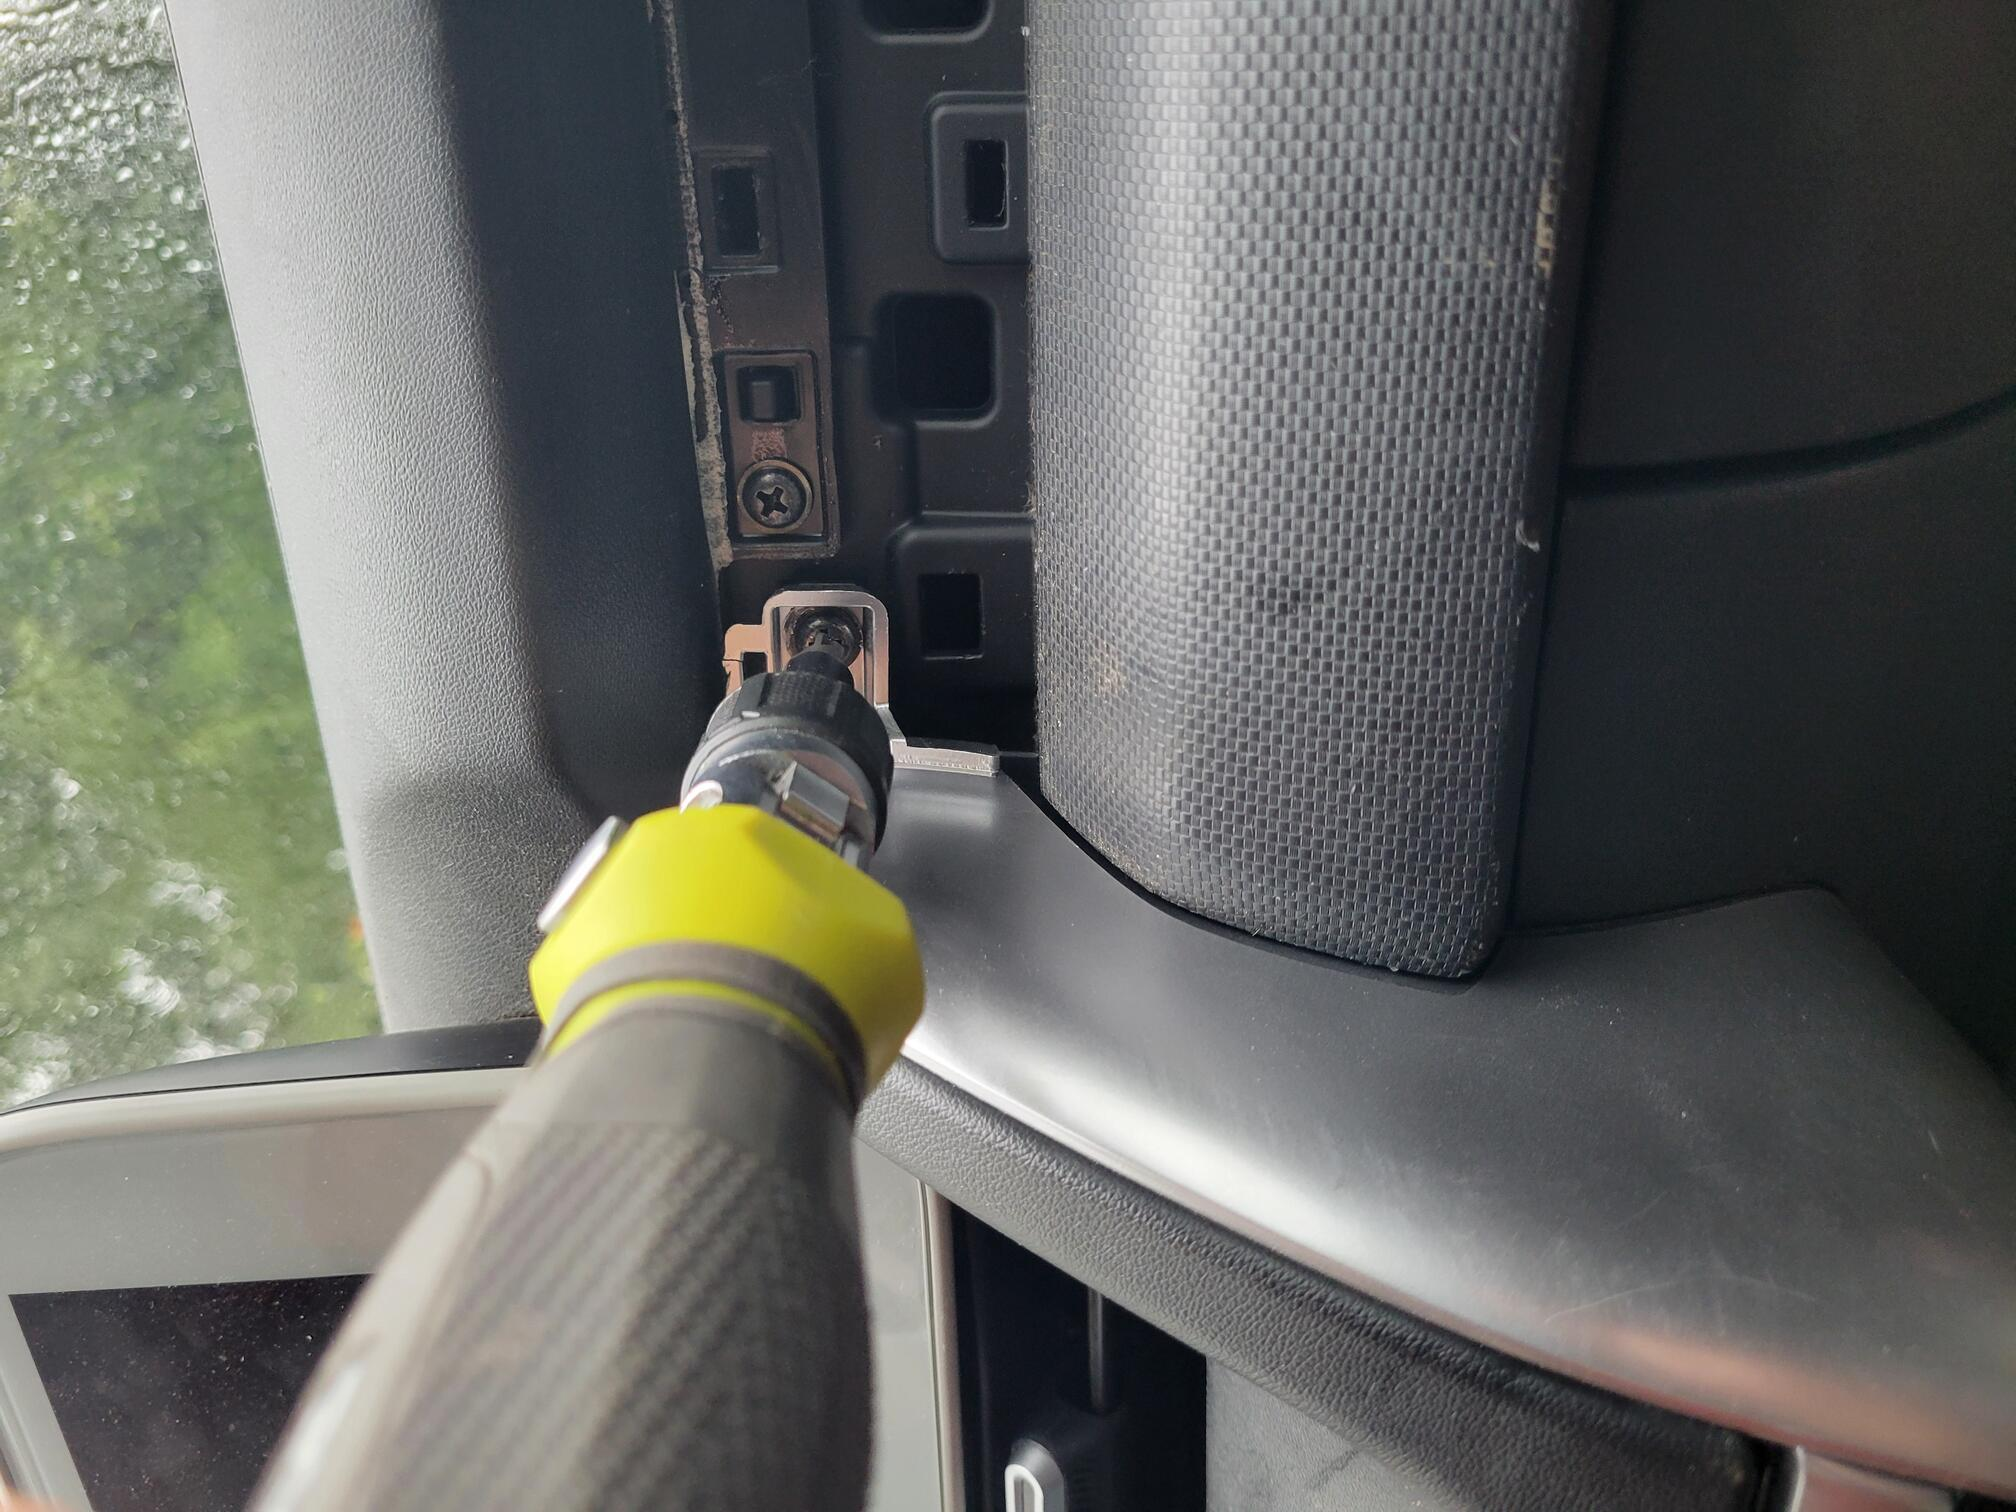
\includegraphics[width=1.5in,angle=-90]{photos/crash_pad_garnish_r_screw.jpg} }  \\
  \subfloat[]{\label{subfig:trimsteps:keyboard_l_screw}
  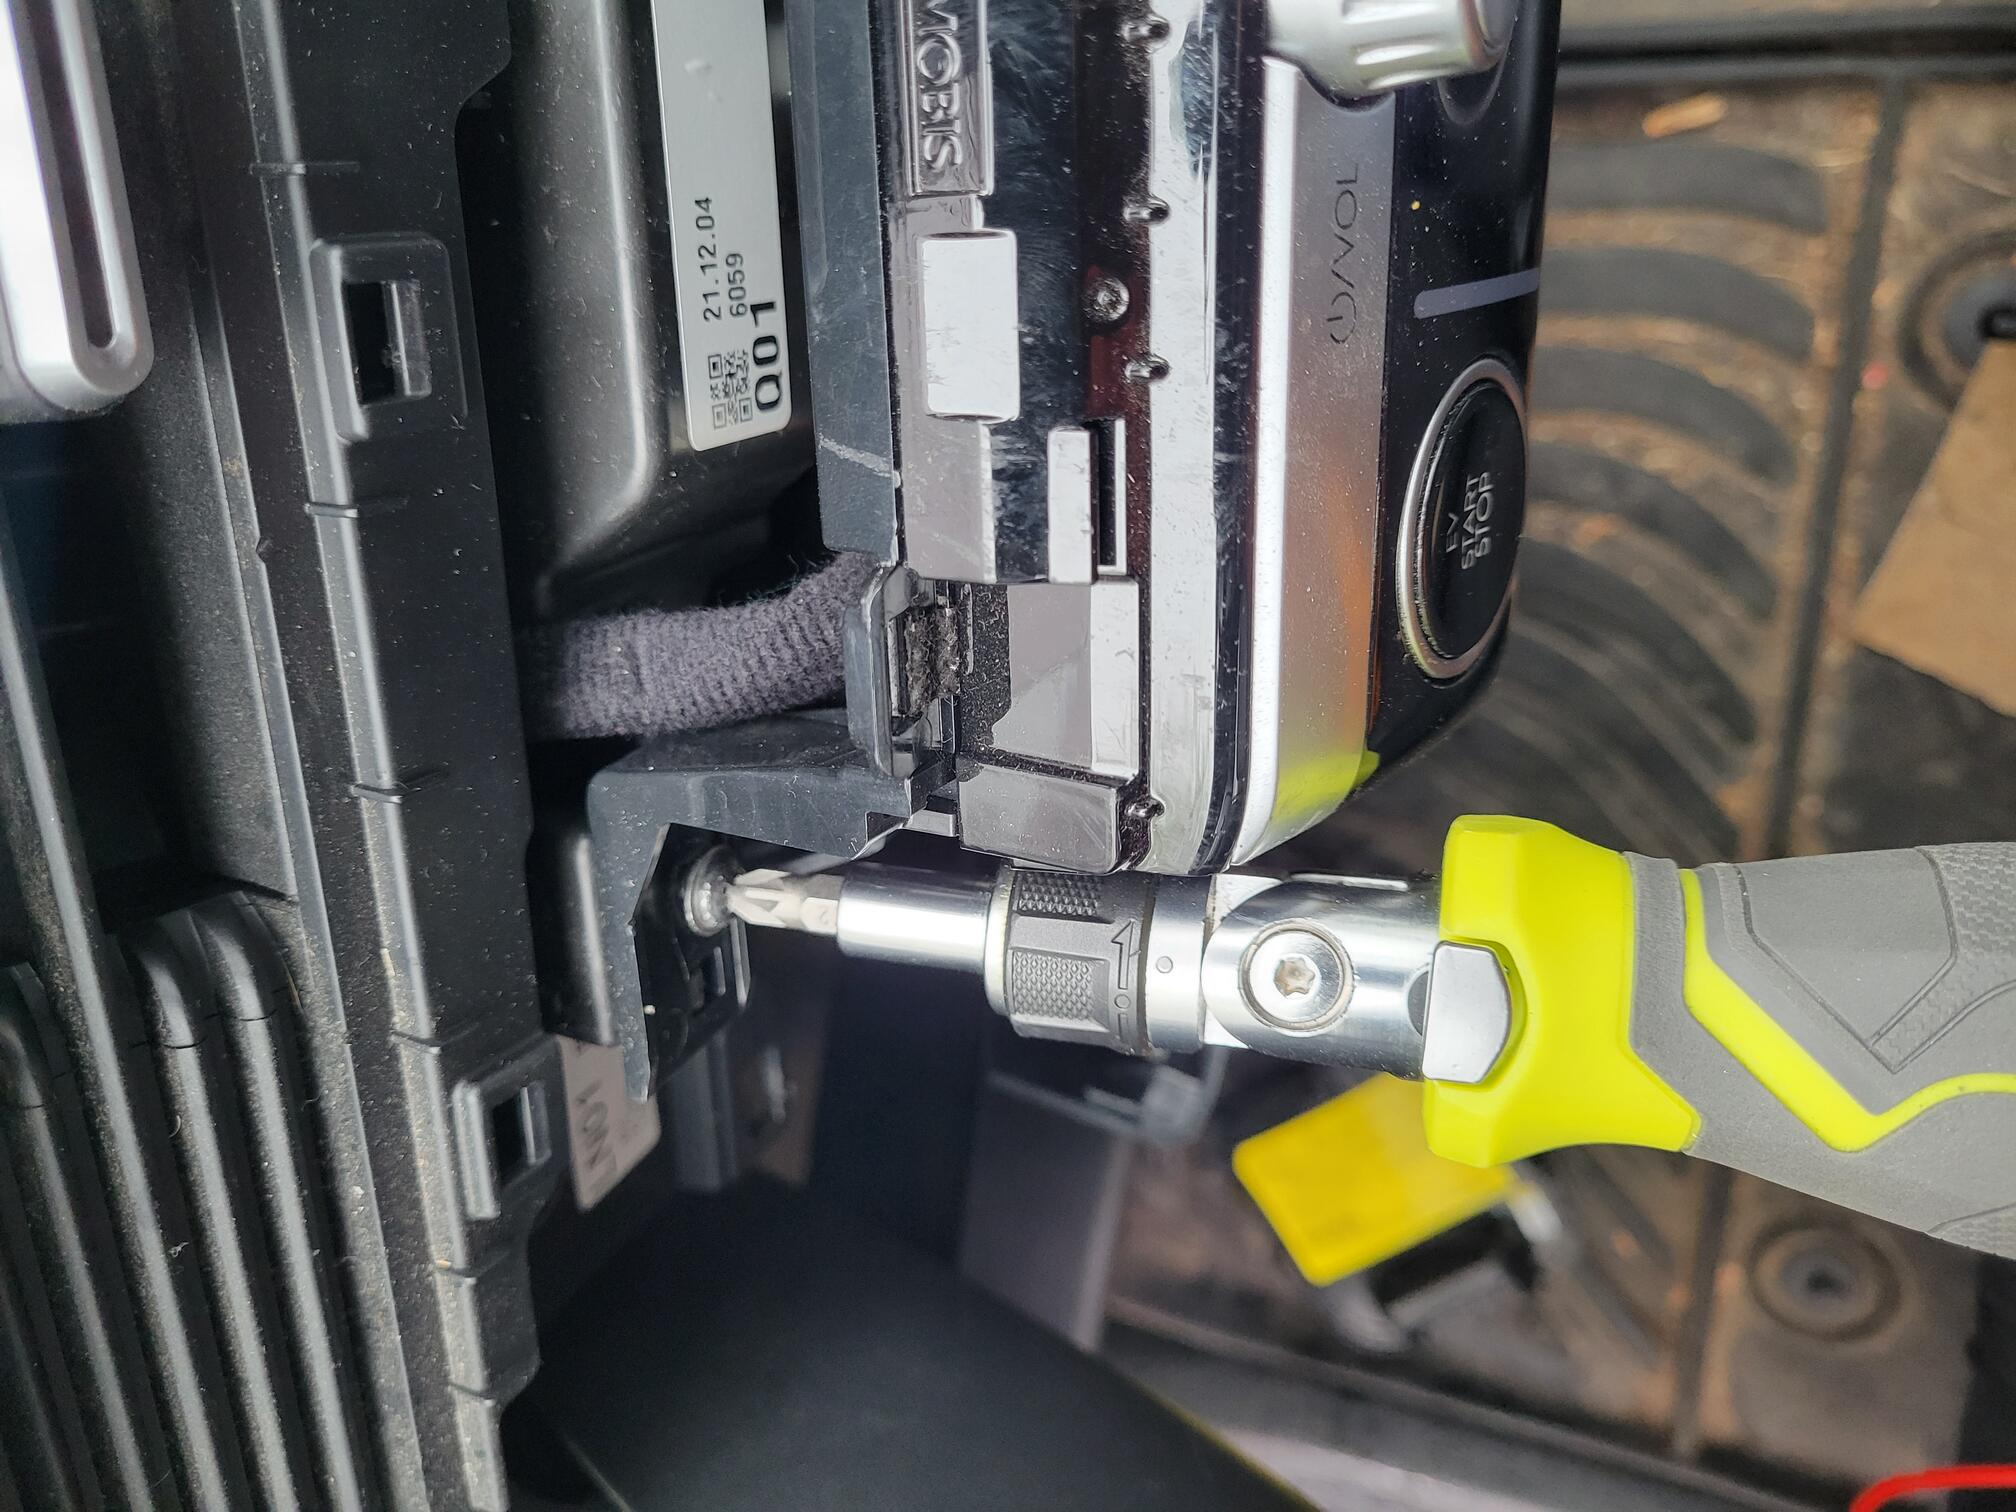
\includegraphics[height=1.5in,angle=180]{photos/keyboard_left_screw.jpg} } 
  \subfloat[]{\label{subfig:trimsteps:keyboard_ur_screw}
  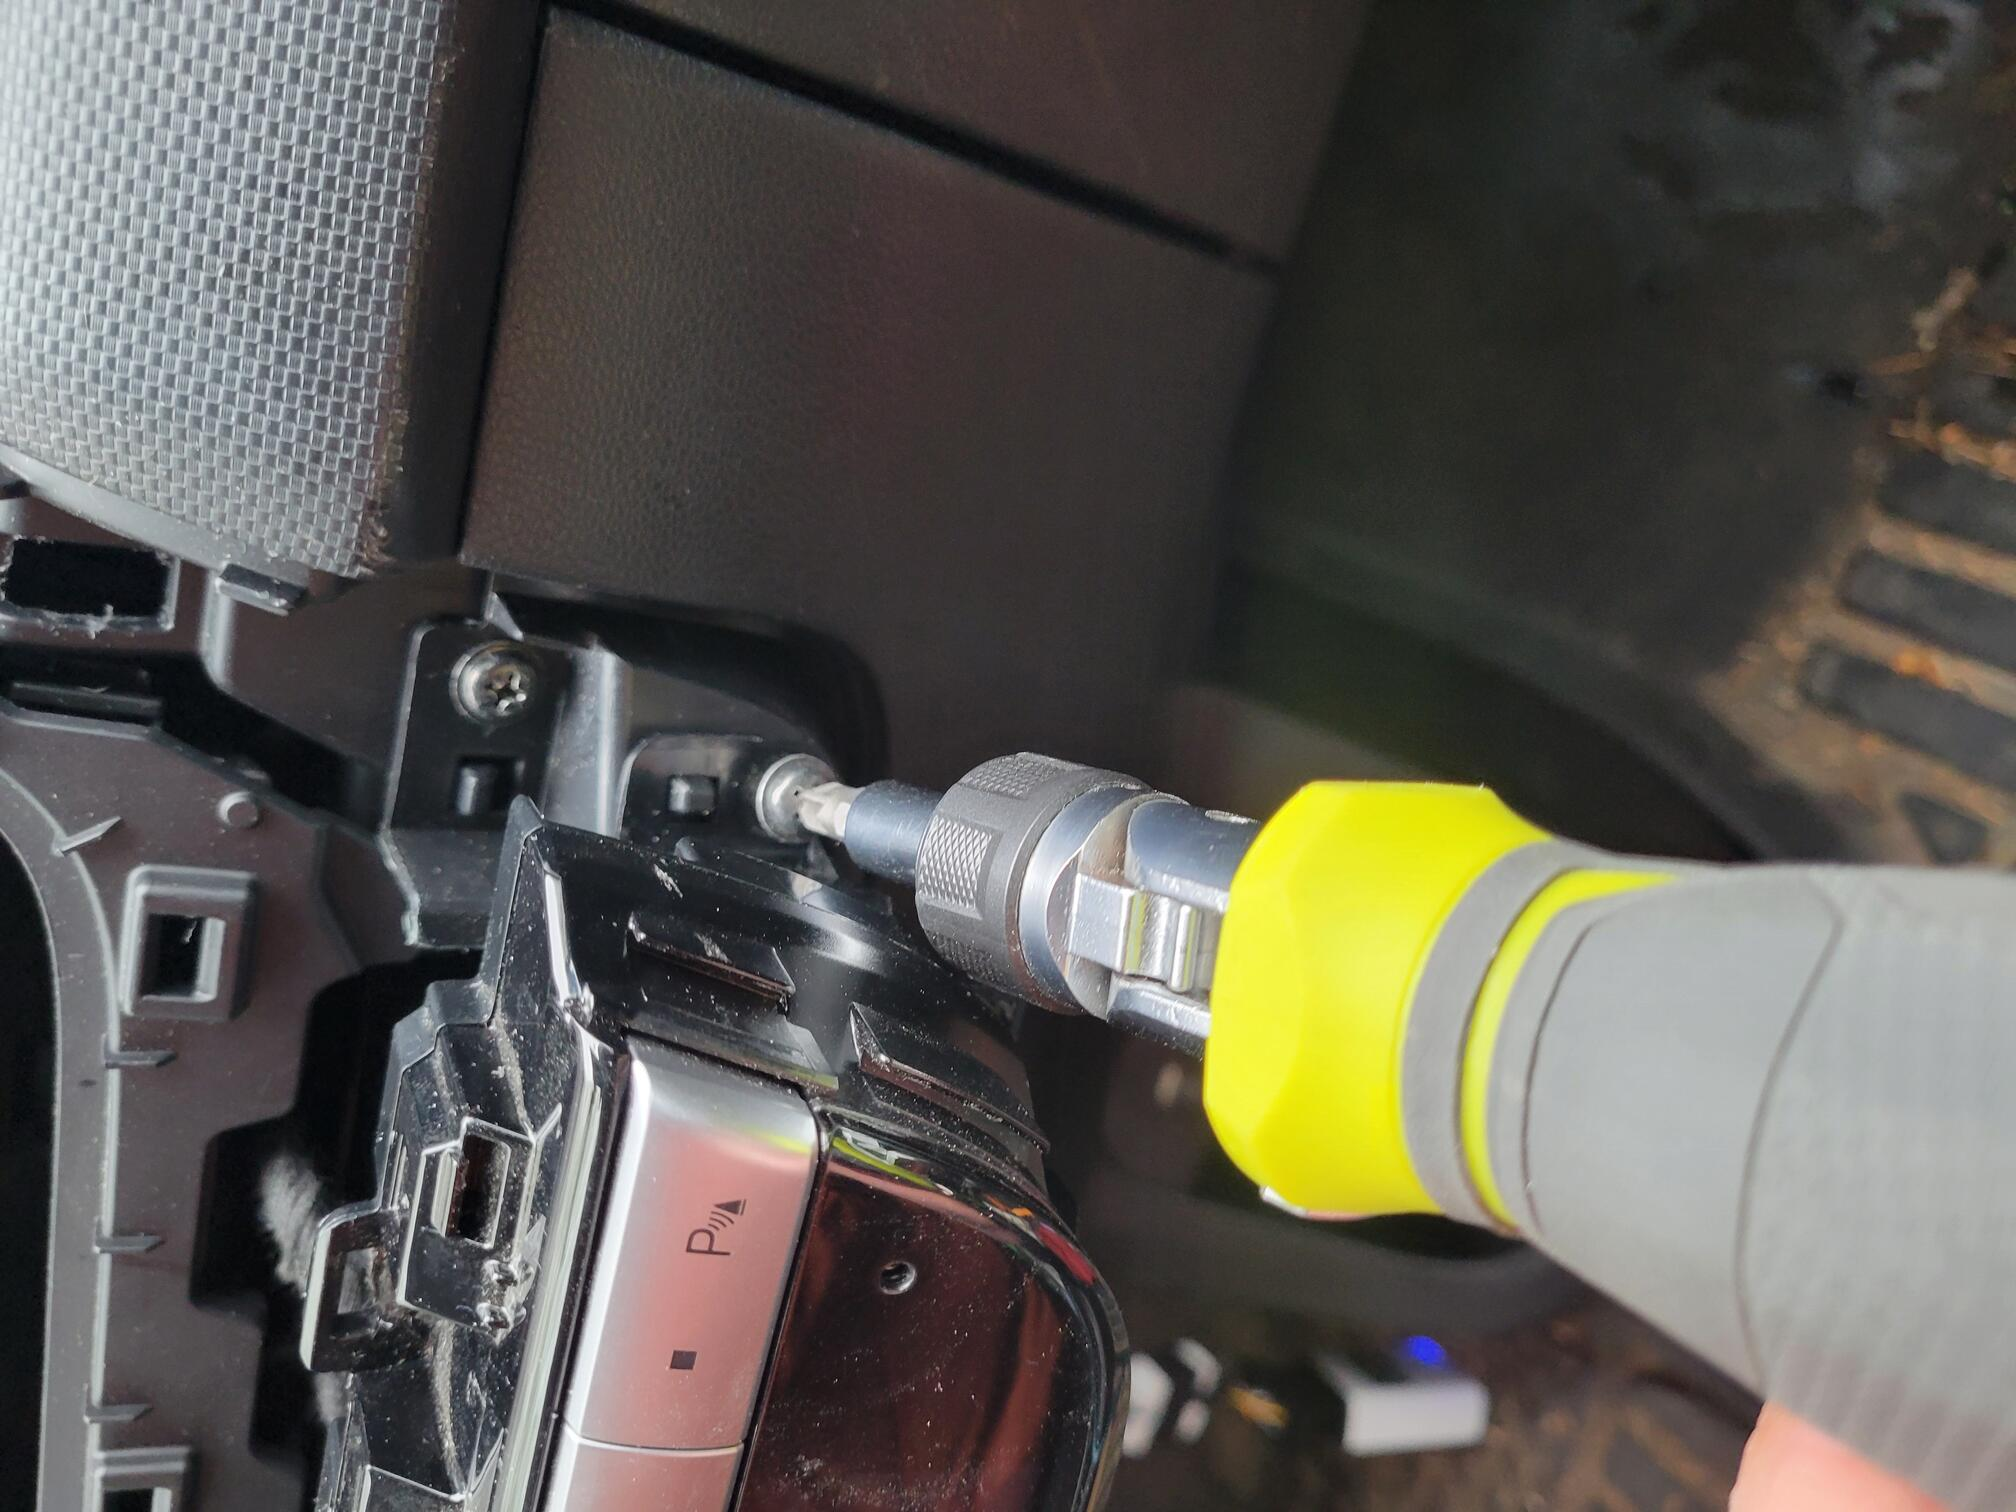
\includegraphics[width=1.5in,angle=-90]{photos/keyboard_ur_screw.jpg} } 
  \subfloat[]{\label{subfig:trimsteps:keyboard_ll_screw}
  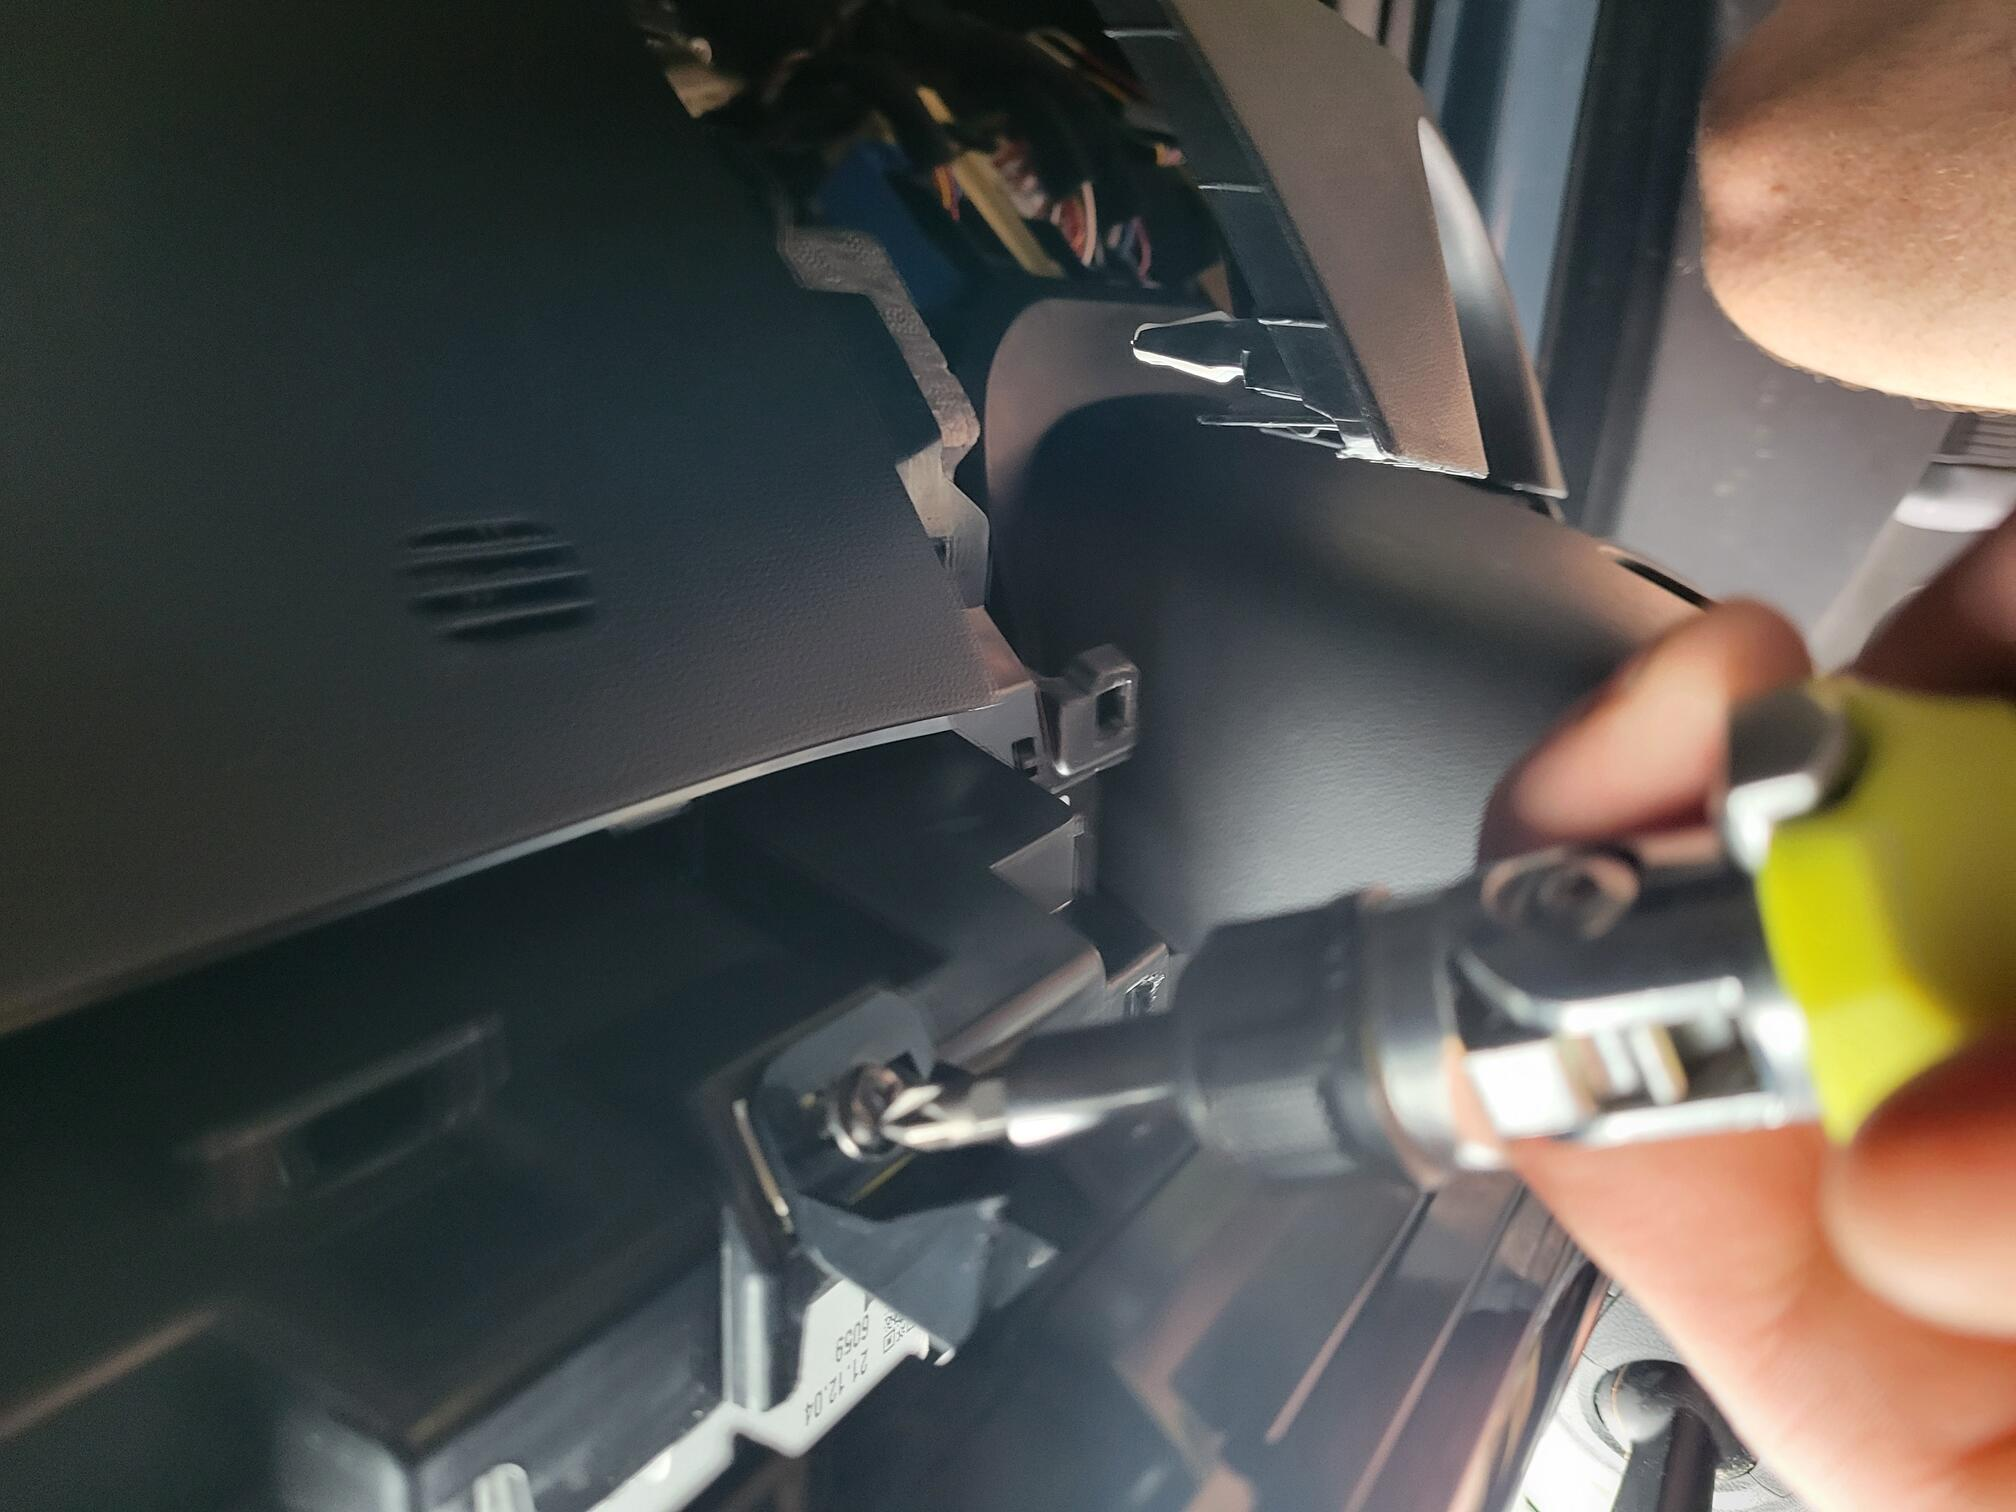
\includegraphics[height=1.5in,angle=180]{photos/keyboard_ll_screw.jpg} }  \\
  \subfloat[]{\label{subfig:trimsteps:keyboard_lr_screw}
  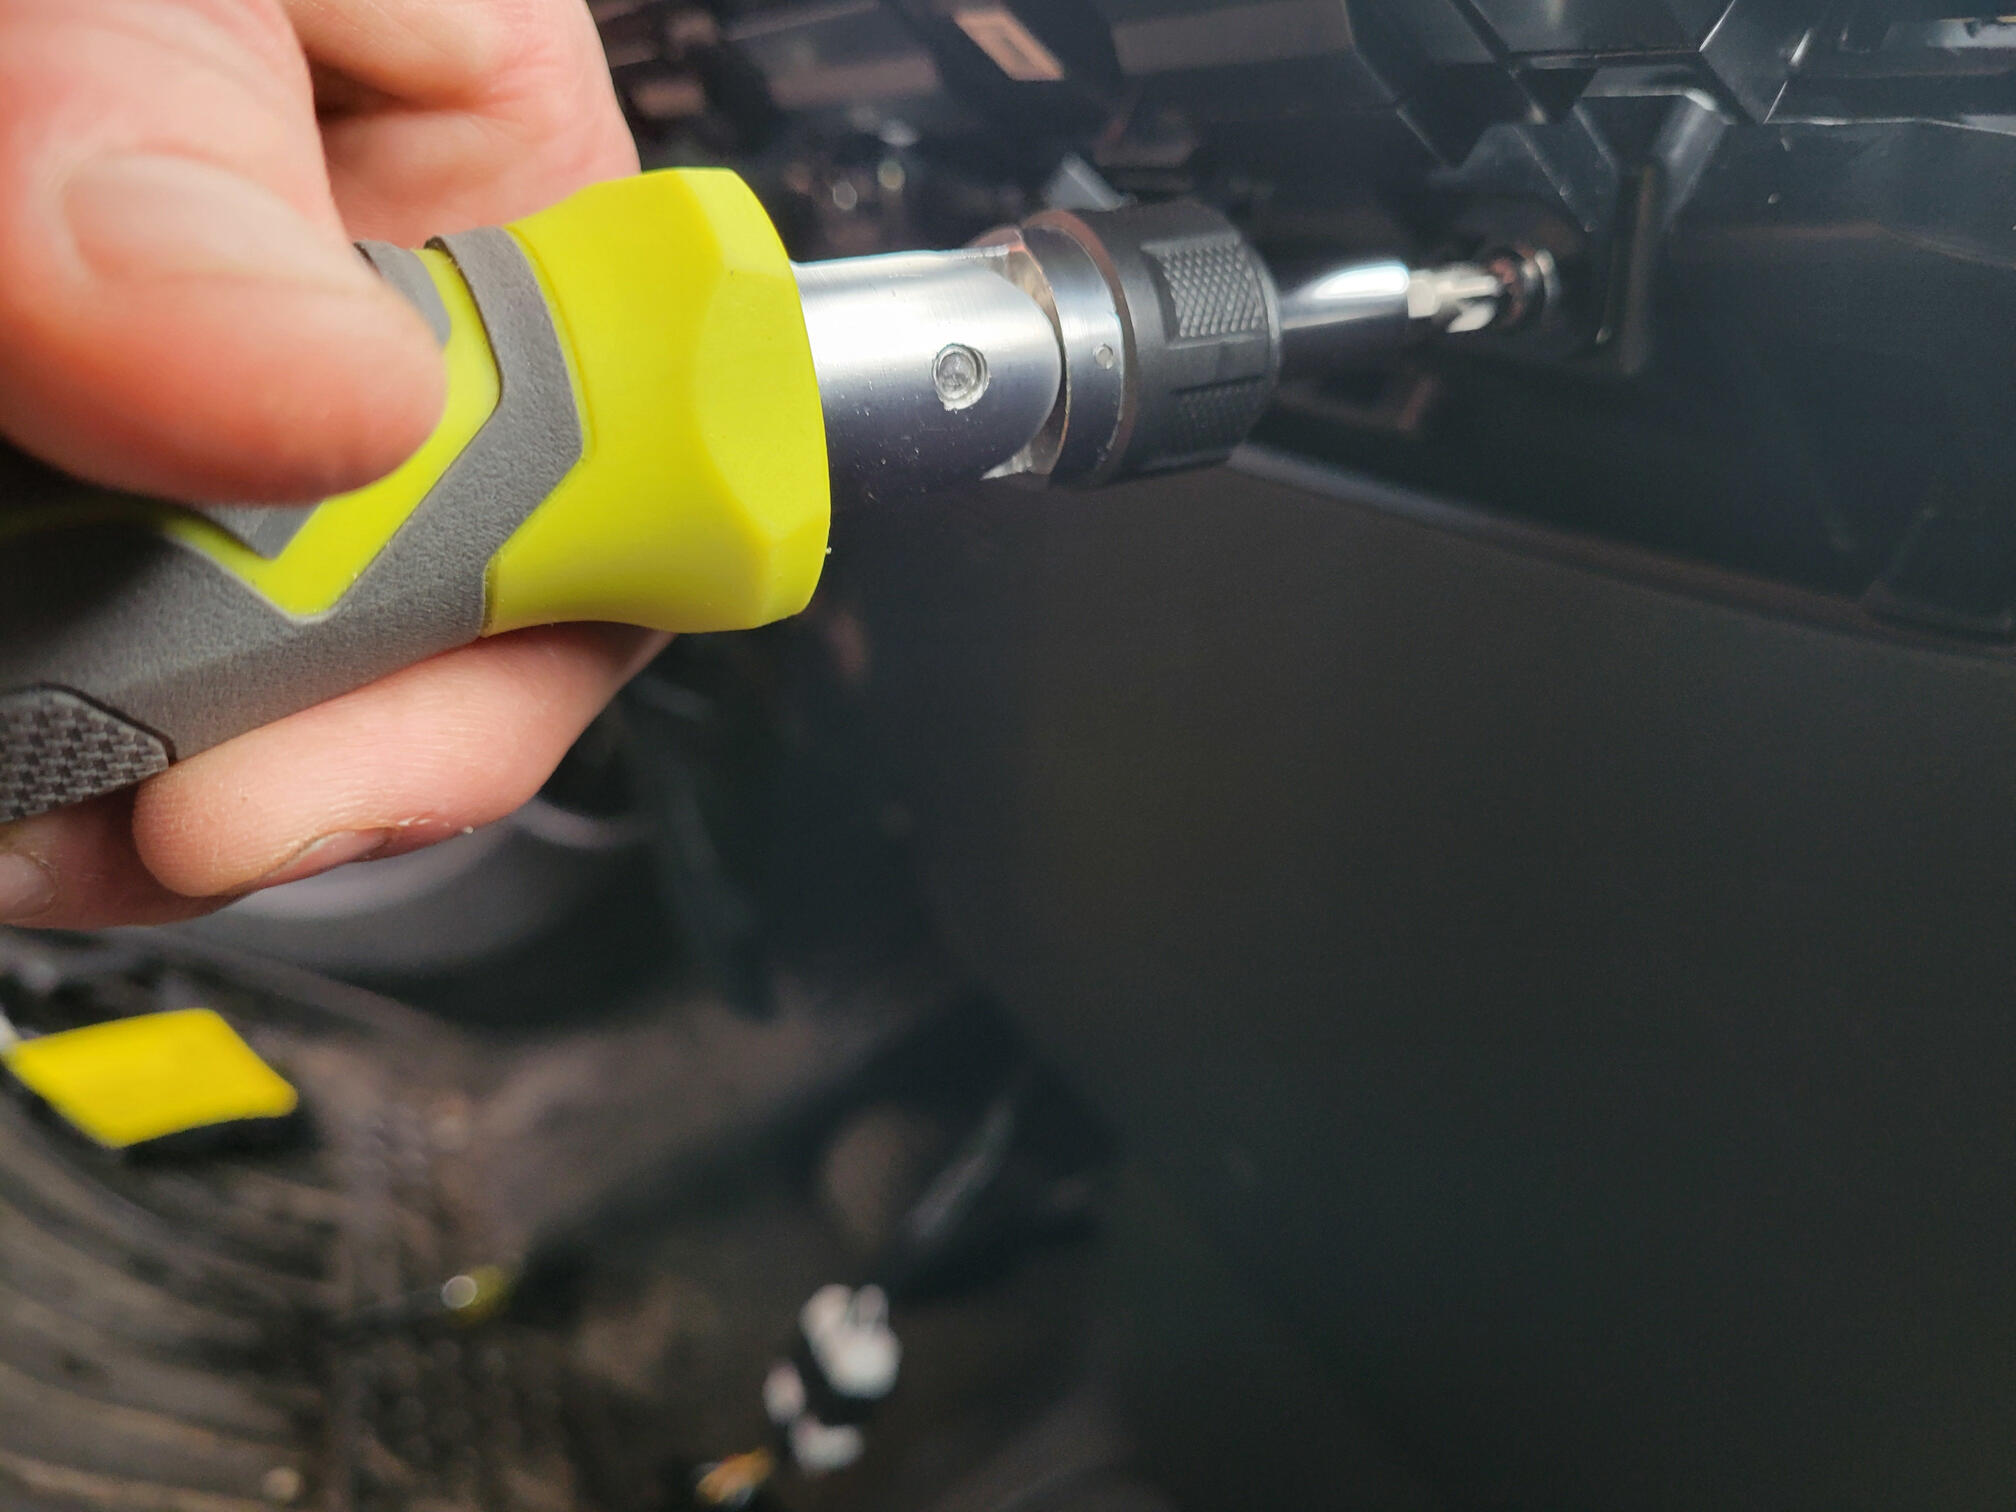
\includegraphics[height=1.5in,angle=0]{photos/keyboard_lr_screw.jpg} } 
  \subfloat[]{\label{subfig:trimsteps:remove_keyboard}
  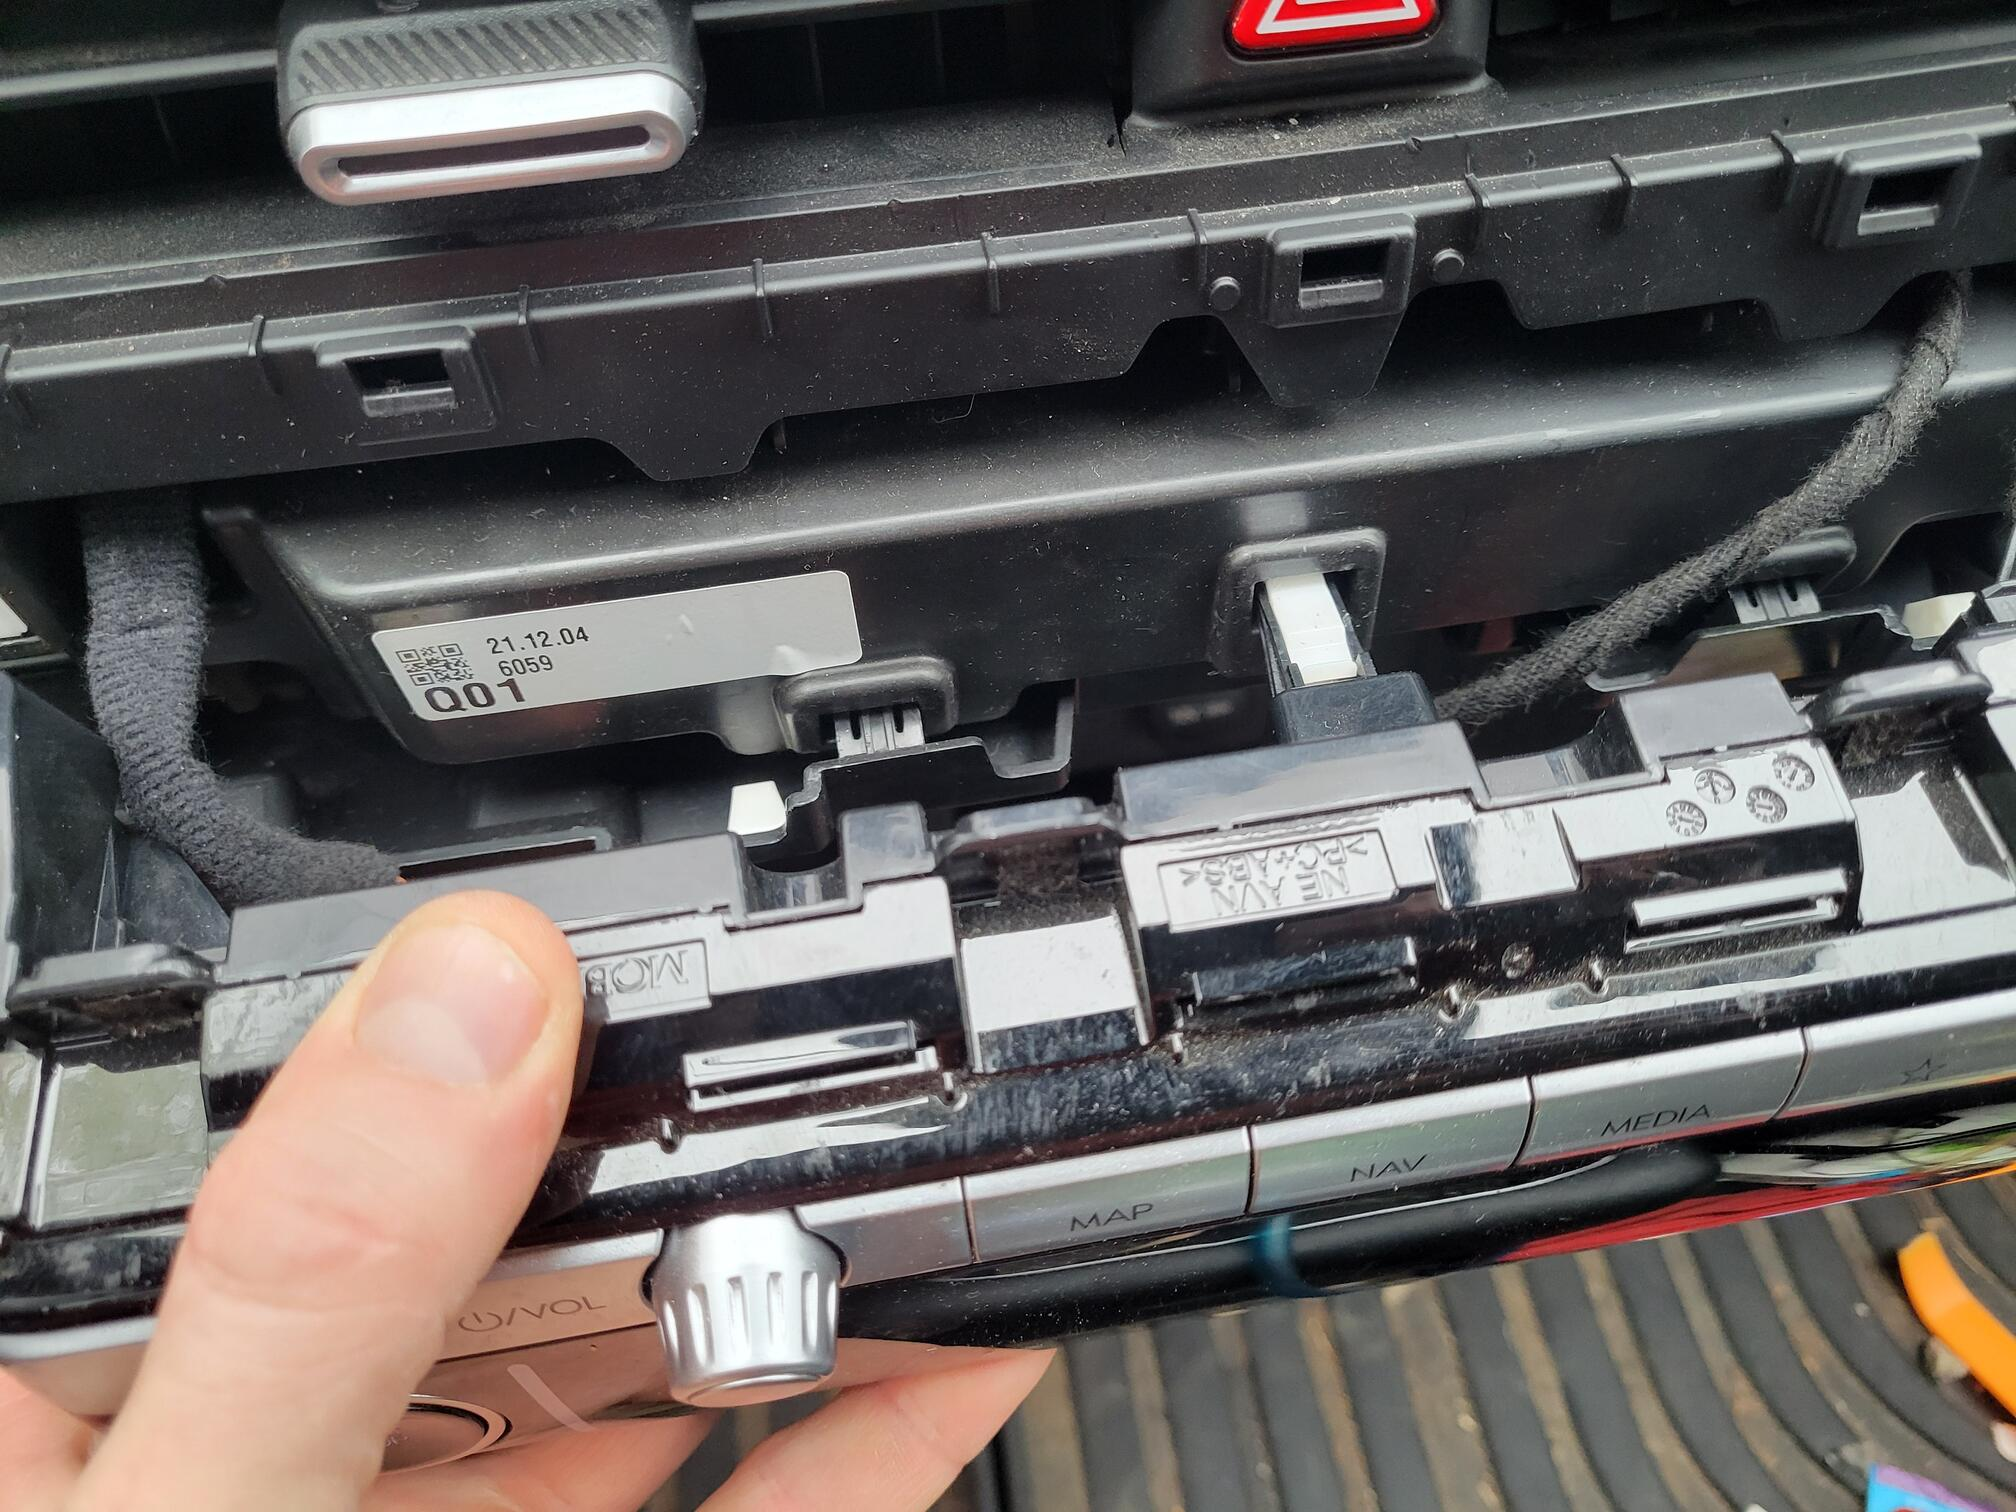
\includegraphics[height=1.5in,angle=0]{photos/remove_keyboard.jpg} }  \\
  \subfloat[]{\label{subfig:trimsteps:cpc_urscrew}
  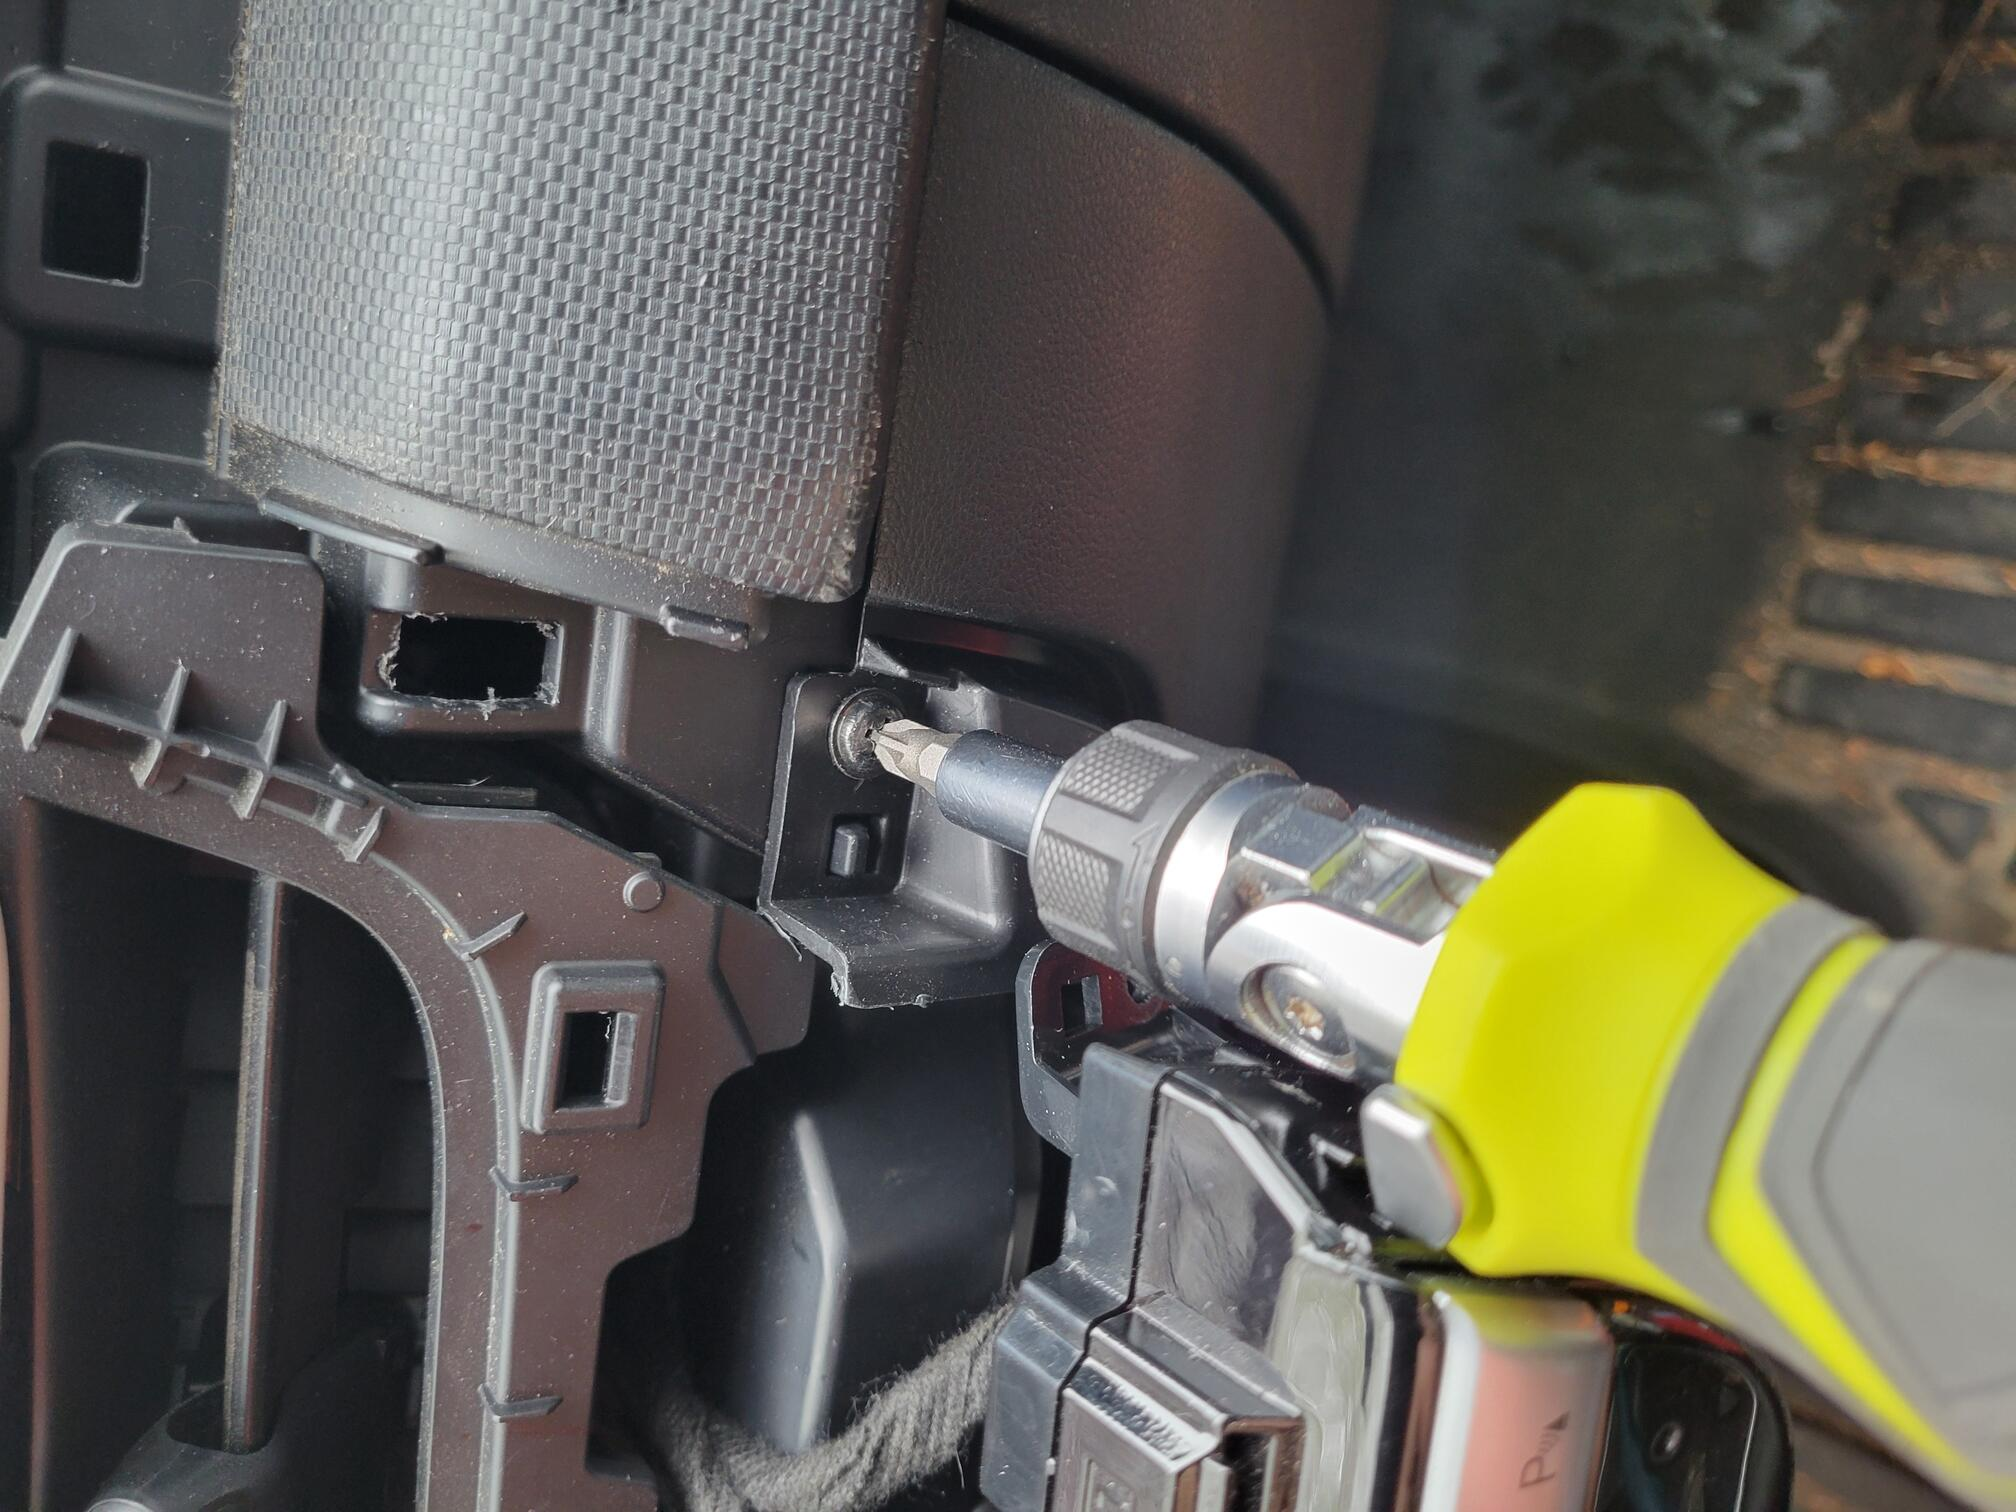
\includegraphics[width=1.5in,angle=-90]{photos/crash_pad_center_ur_screw.jpg} }  
  \subfloat[]{\label{subfig:trimsteps:cpc_ulscrew}
  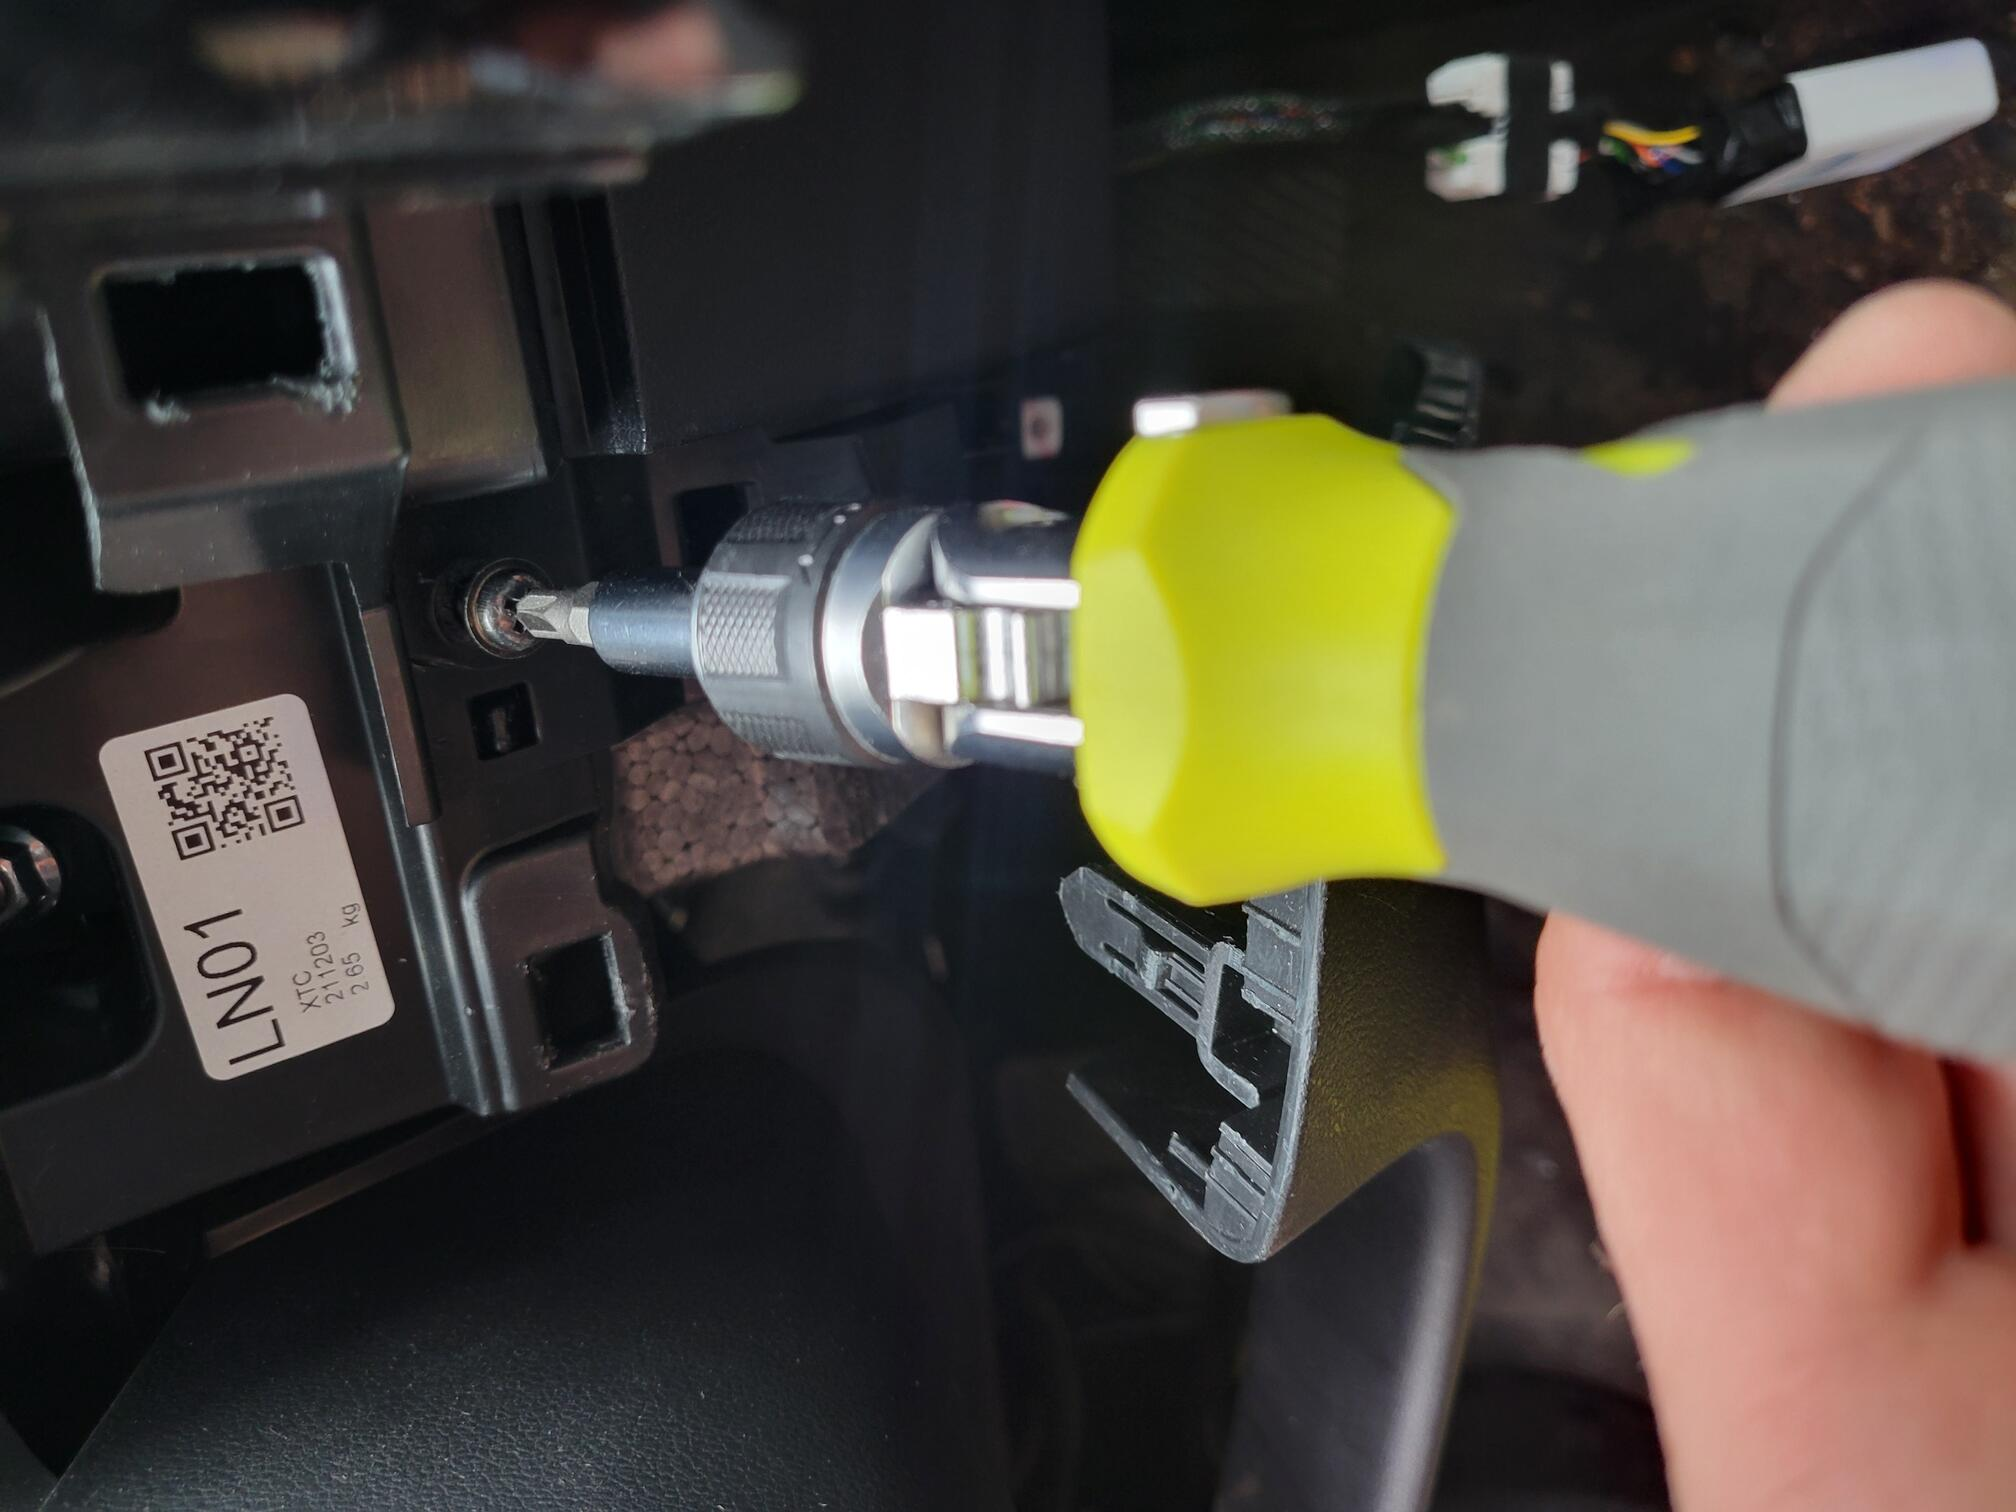
\includegraphics[width=1.5in,angle=-90]{photos/crash_pad_center_ul_screw.jpg} } 
   \caption{(a) Dépose de la vis du crash pad inférieur. (b) Vous pouvez trouver une ou deux vis derrière le crash pad inférieur. (c) Dépose de la ou des vis derrière le crash pad inférieur. (d) Dépose de la vis retenant la garniture du crash pad. (e) Retrait de la vis gauche du clavier AVN. (f) Retrait de la vis droite du clavier AVN. (g) Retrait de la vis inférieure gauche du clavier AVN. (h) Retrait de la vis inférieure droite du clavier AVN. (i) Suppression du clavier AVN. (j) Retrait de la vis centrale du crash pad qui était bloquée par le clavier AVN. (k) Retrait de la vis centrale du crash pad qui se trouvait derrière la garniture du crash pad, à gauche du clavier AVN. \label{fig:trimsteps}}
\end{figure}
\subsection{Option B : rapide}
Nous ne supprimons que partiellement deux panneaux de garniture avec cette approche :
\begin{enumerate}
  \item Crash pad inférieur
  \item Centre de crash pad
\end{enumerate}
Notez que la garniture du crash pad peut encore se détacher lors de l'installation. Il peut être réactivé une fois terminé.

Instructions étape par étape :
\begin{enumerate}
  \item Retirez la vis du crash pad inférieur (Figure \ref{subfig:trimsteps:lowerscrew})
  \item Retirez la moitié droite du crash pad inférieur à l'aide de l'outil de dépose de garniture. 
  \item Pendant que vous êtes ici, retirez la ou les vis derrière le crash pad inférieur (il peut y en avoir 1 ou 2 ; voir la figure \ref{subfig:trimsteps:cpc_llscrews}); la vis la plus à gauche fixée à l'évent derrière a tendance à rester captive, vous devez donc tirer pour confirmer qu'elle est retirée (Figure \ref{subfig:trimsteps:cpc_llscrew})
  \item Retirez le bas du centre du crash pad
  \item Vous pouvez maintenant accéder à l'unité principale par le dessous du centre du crash pad.
\end{enumerate}

\subsection{Option C : option rapide 2}

Cette méthode n'est pas recommandée, mais présentée ici à titre d'information. Raisons à éviter :
\begin{enumerate}
  \item Nécessite un long tournevis droit pour une douille de 10 mm
  \item N'offre pas un accès aussi bon que l'option B (mais pourrait être combiné avec l'option B)
  \item La réinstallation des garnitures est plus délicate ; l'alignement des 3 clips en haut est difficile. 
\end{enumerate}
L’avantage principal de cette méthode est que des points de montage bien cachés sont possibles. Ceux-ci ne sont pas documentés ici, mais le \href{https://github.com/tylerharvey/Ioniq5_CAN/blob/main/guides/cars/E-GMP_gen1/EV6/head_unit_preconditioning_kit_EV6_install.pdf}{Manuel d'installation EV6} propose quelques idées. Dans cette méthode, nous retirons le plateau inférieur central du crash pad, le boîtier du port USB avant. 

\begin{enumerate}
  \item Retirez le clip de garniture gauche avec l'outil de dépose de garniture (Figure \ref{subfig:usb_trim:left_clip})
  \item Retirez le clip de garniture droit à l'aide de l'outil de dépose de garniture (Figure \ref{subfig:usb_trim:right_clip})
  \item Retirez le plancher du rangement de la console à l'aide de l'outil de dépose de garniture (Figure \ref{subfig:usb_trim:carpet}) 
  \item Retirez le boulon avec la douille de 10 mm sur un long tournevis droit (Figure \ref{subfig:usb_trim:bolt})
  \item Soulevez le haut du plateau inférieur central du crash pad pour déconnecter les 3 clips de garniture en haut (Figure \ref{subfig:usb_trim:trim_off})
  \item Mettez-le de côté (Figure \ref{subfig:usb_trim:trim_to_side})
\end{enumerate}

\begin{figure}[h]
  \subfloat[]{\label{subfig:usb_trim:left_clip}
  \includegraphics[height=1.5in,angle=0]{photos/usb_trim_clip_left.jpg} } 
  \subfloat[]{\label{subfig:usb_trim:right_clip}
  \includegraphics[height=1.5in,angle=0]{photos/usb_trim_clip_right.jpg} } 
  \subfloat[]{\label{subfig:usb_trim:carpet}
  \includegraphics[height=1.5in,angle=0]{photos/removing_usb_trim_carpet.jpg} } \\
  \subfloat[]{\label{subfig:usb_trim:bolt}
  \includegraphics[height=1.5in,angle=0]{photos/removing_usb_trim_bolt.jpg} } 
  \subfloat[]{\label{subfig:usb_trim:trim_off}
  \includegraphics[height=1.5in,angle=0]{photos/usb_trim_off_2.jpg} } 
  \subfloat[]{\label{subfig:usb_trim:trim_to_side}
  \includegraphics[height=1.5in,angle=0]{photos/usb_trim_off.jpg} }  
  \subfloat[]{\label{subfig:usb_trim:HU}
  \includegraphics[height=1.5in,angle=0]{photos/usb_trim_off_reaching_for_HU.jpg} } 
   \caption{Retrait du plateau inférieur central du crash pad : (a) Clip gauche. (b) Clip droit. (c) Enlèvement du plancher. (d) Retirez le boulon avec une douille de 10 mm. (e) Débranchez les 3 clips de garniture avec l'outil de dépose de garniture. (f) Placez la garniture sur le côté. (g) Vous pouvez maintenant atteindre le bas de l'unité principale.  \label{fig:usb_trim}}
\end{figure}
\section{Étape 3 : Connexion du faisceau} \label{sect:2}
Cette étape couvre l'installation du harnais dans l'unité principale. 

Instructions étape par étape :
\begin{enumerate}
  \item Identifiez le connecteur gris d'origine de l'unité principale femelle (Figure \ref{subfig:harness:headunit})
  \item Retirez-le en appuyant sur le clip et en le tirant vers le bas (Figure \ref{subfig:harness:M05Bout})
  \item Insérez le côté femelle du harnais dans l'unité principale (Figure \ref{subfig:harness:female})
  \item Insérez le connecteur femelle que vous avez retiré dans le côté mâle du faisceau (Figure \ref{subfig:harness:harness_in})
\end{enumerate}

\begin{figure}[h]
  \subfloat[]{\label{subfig:harness:female}
  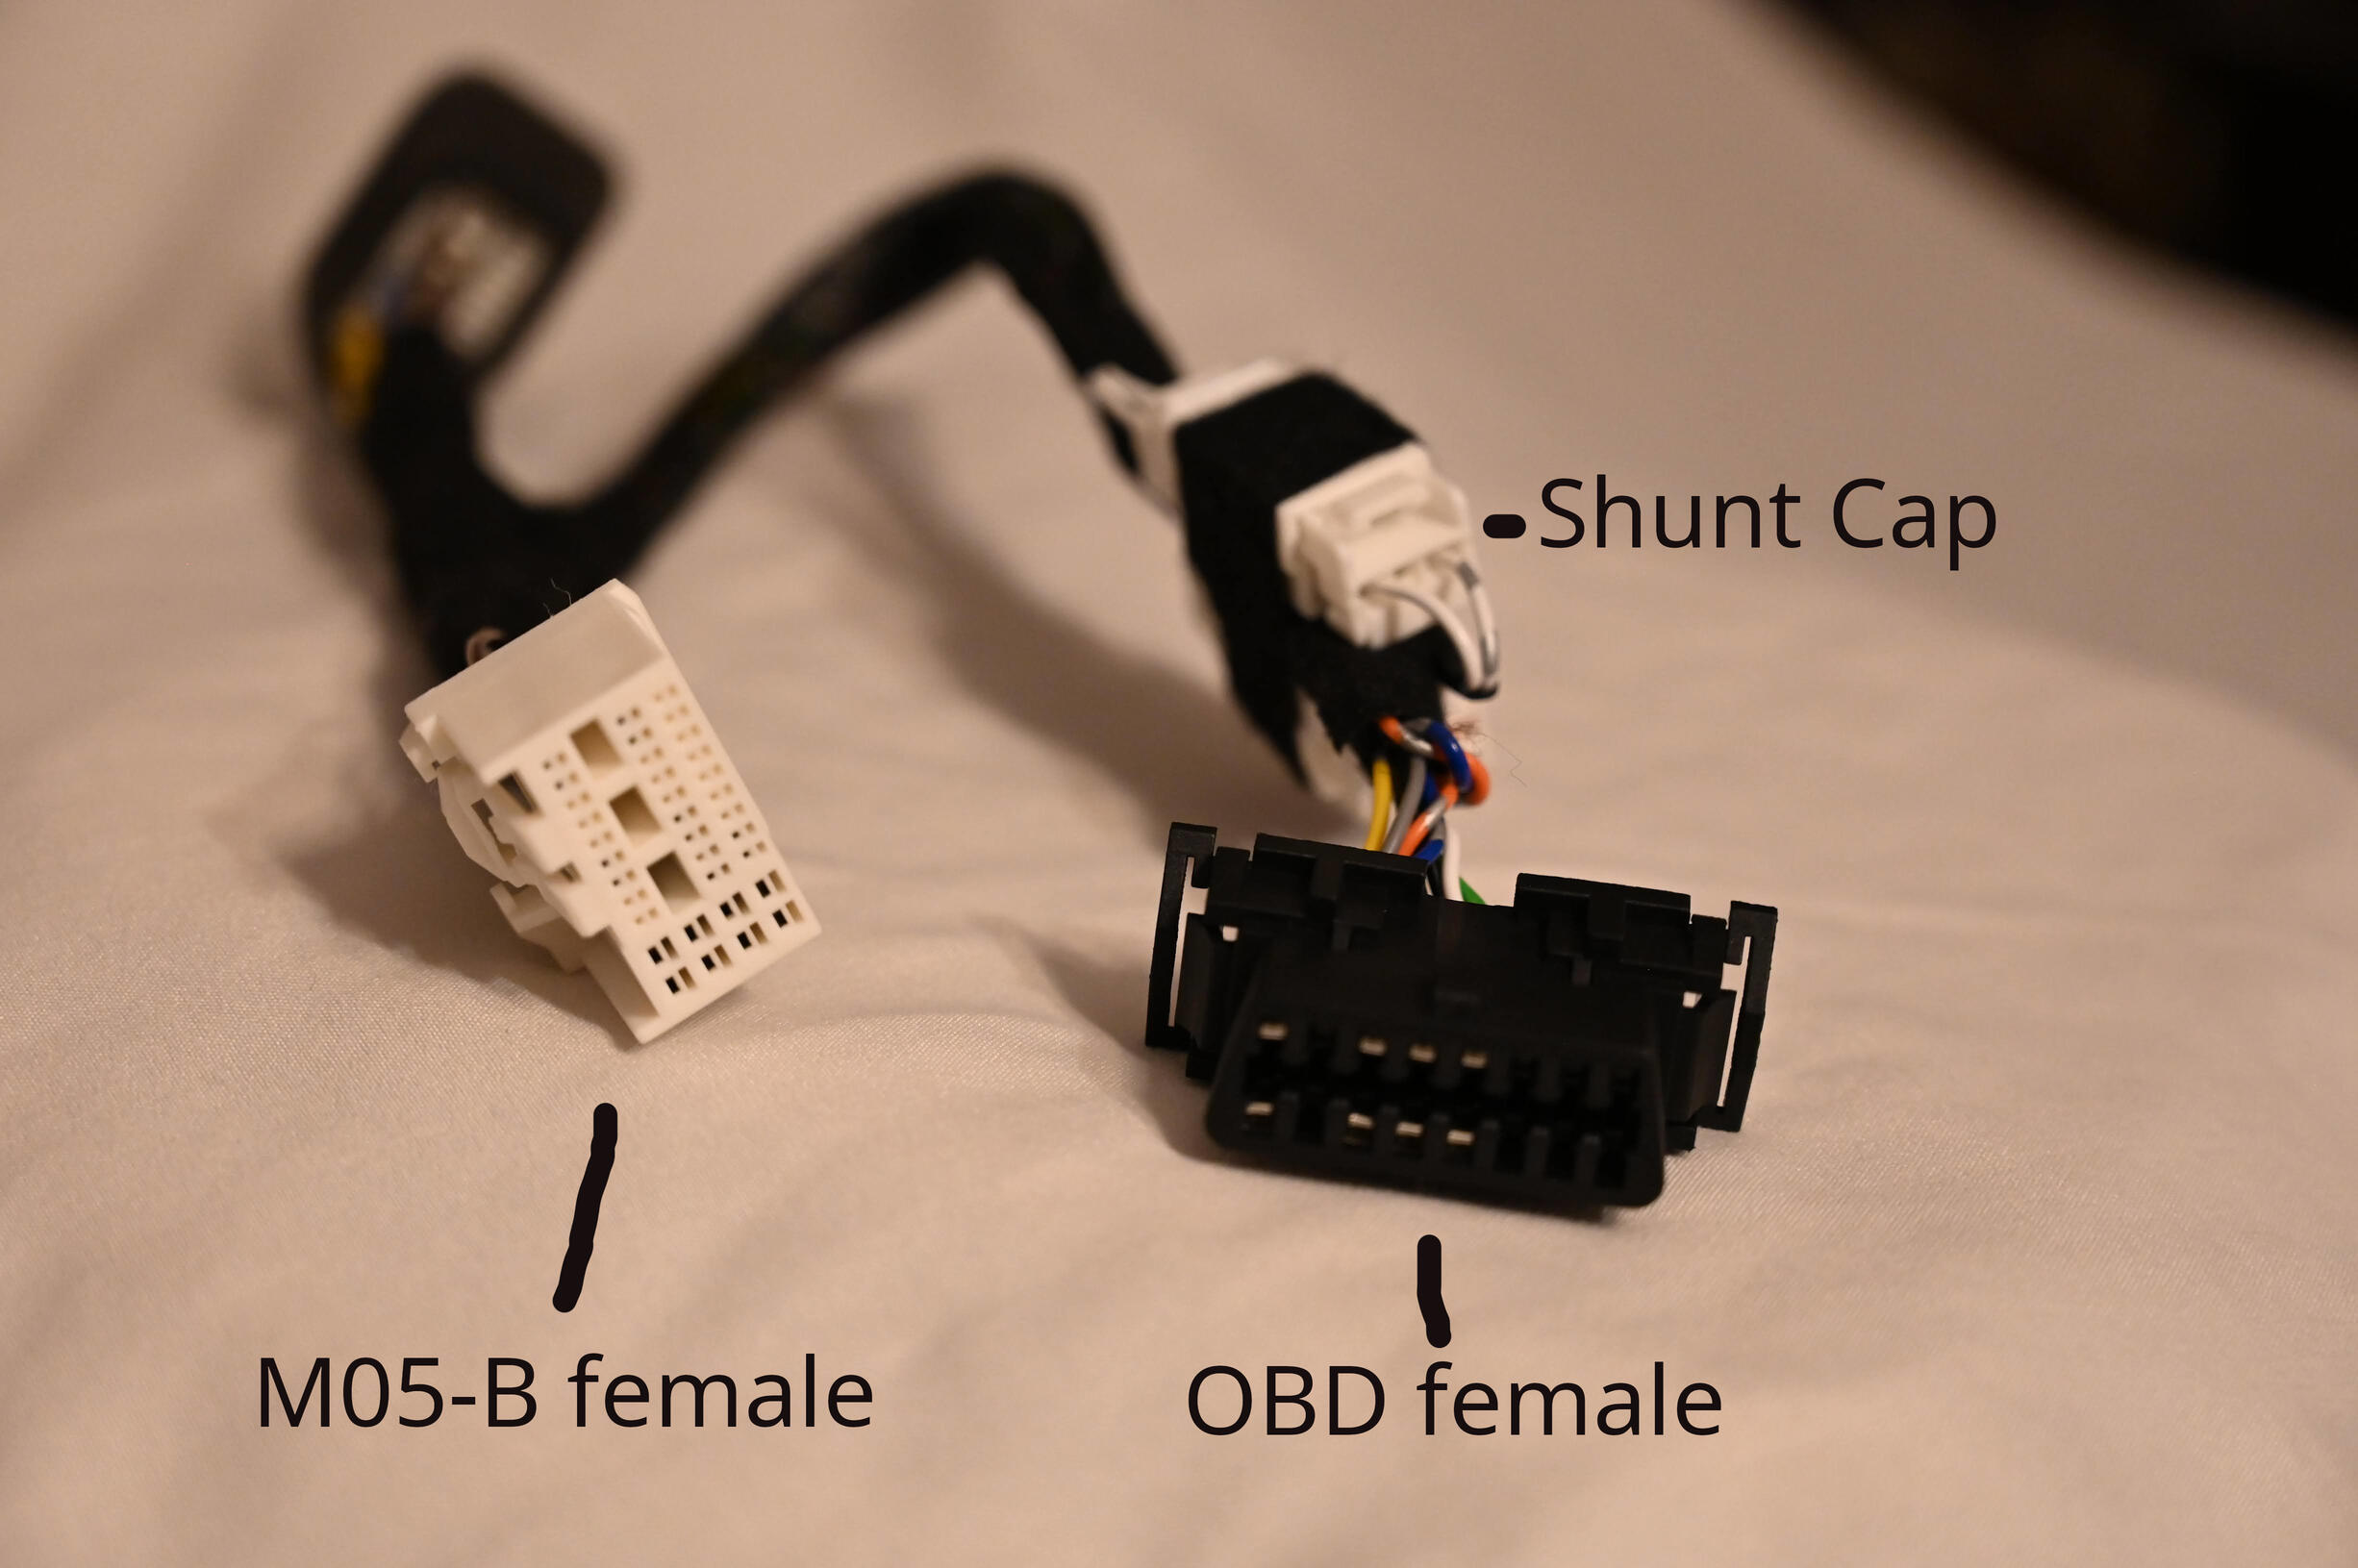
\includegraphics[height=1.5in,angle=0]{../../../harnesses/head_unit_MITM/photos/labeled_connectors_MITM_harness.jpg} } 
  \subfloat[]{\label{subfig:harness:male}
  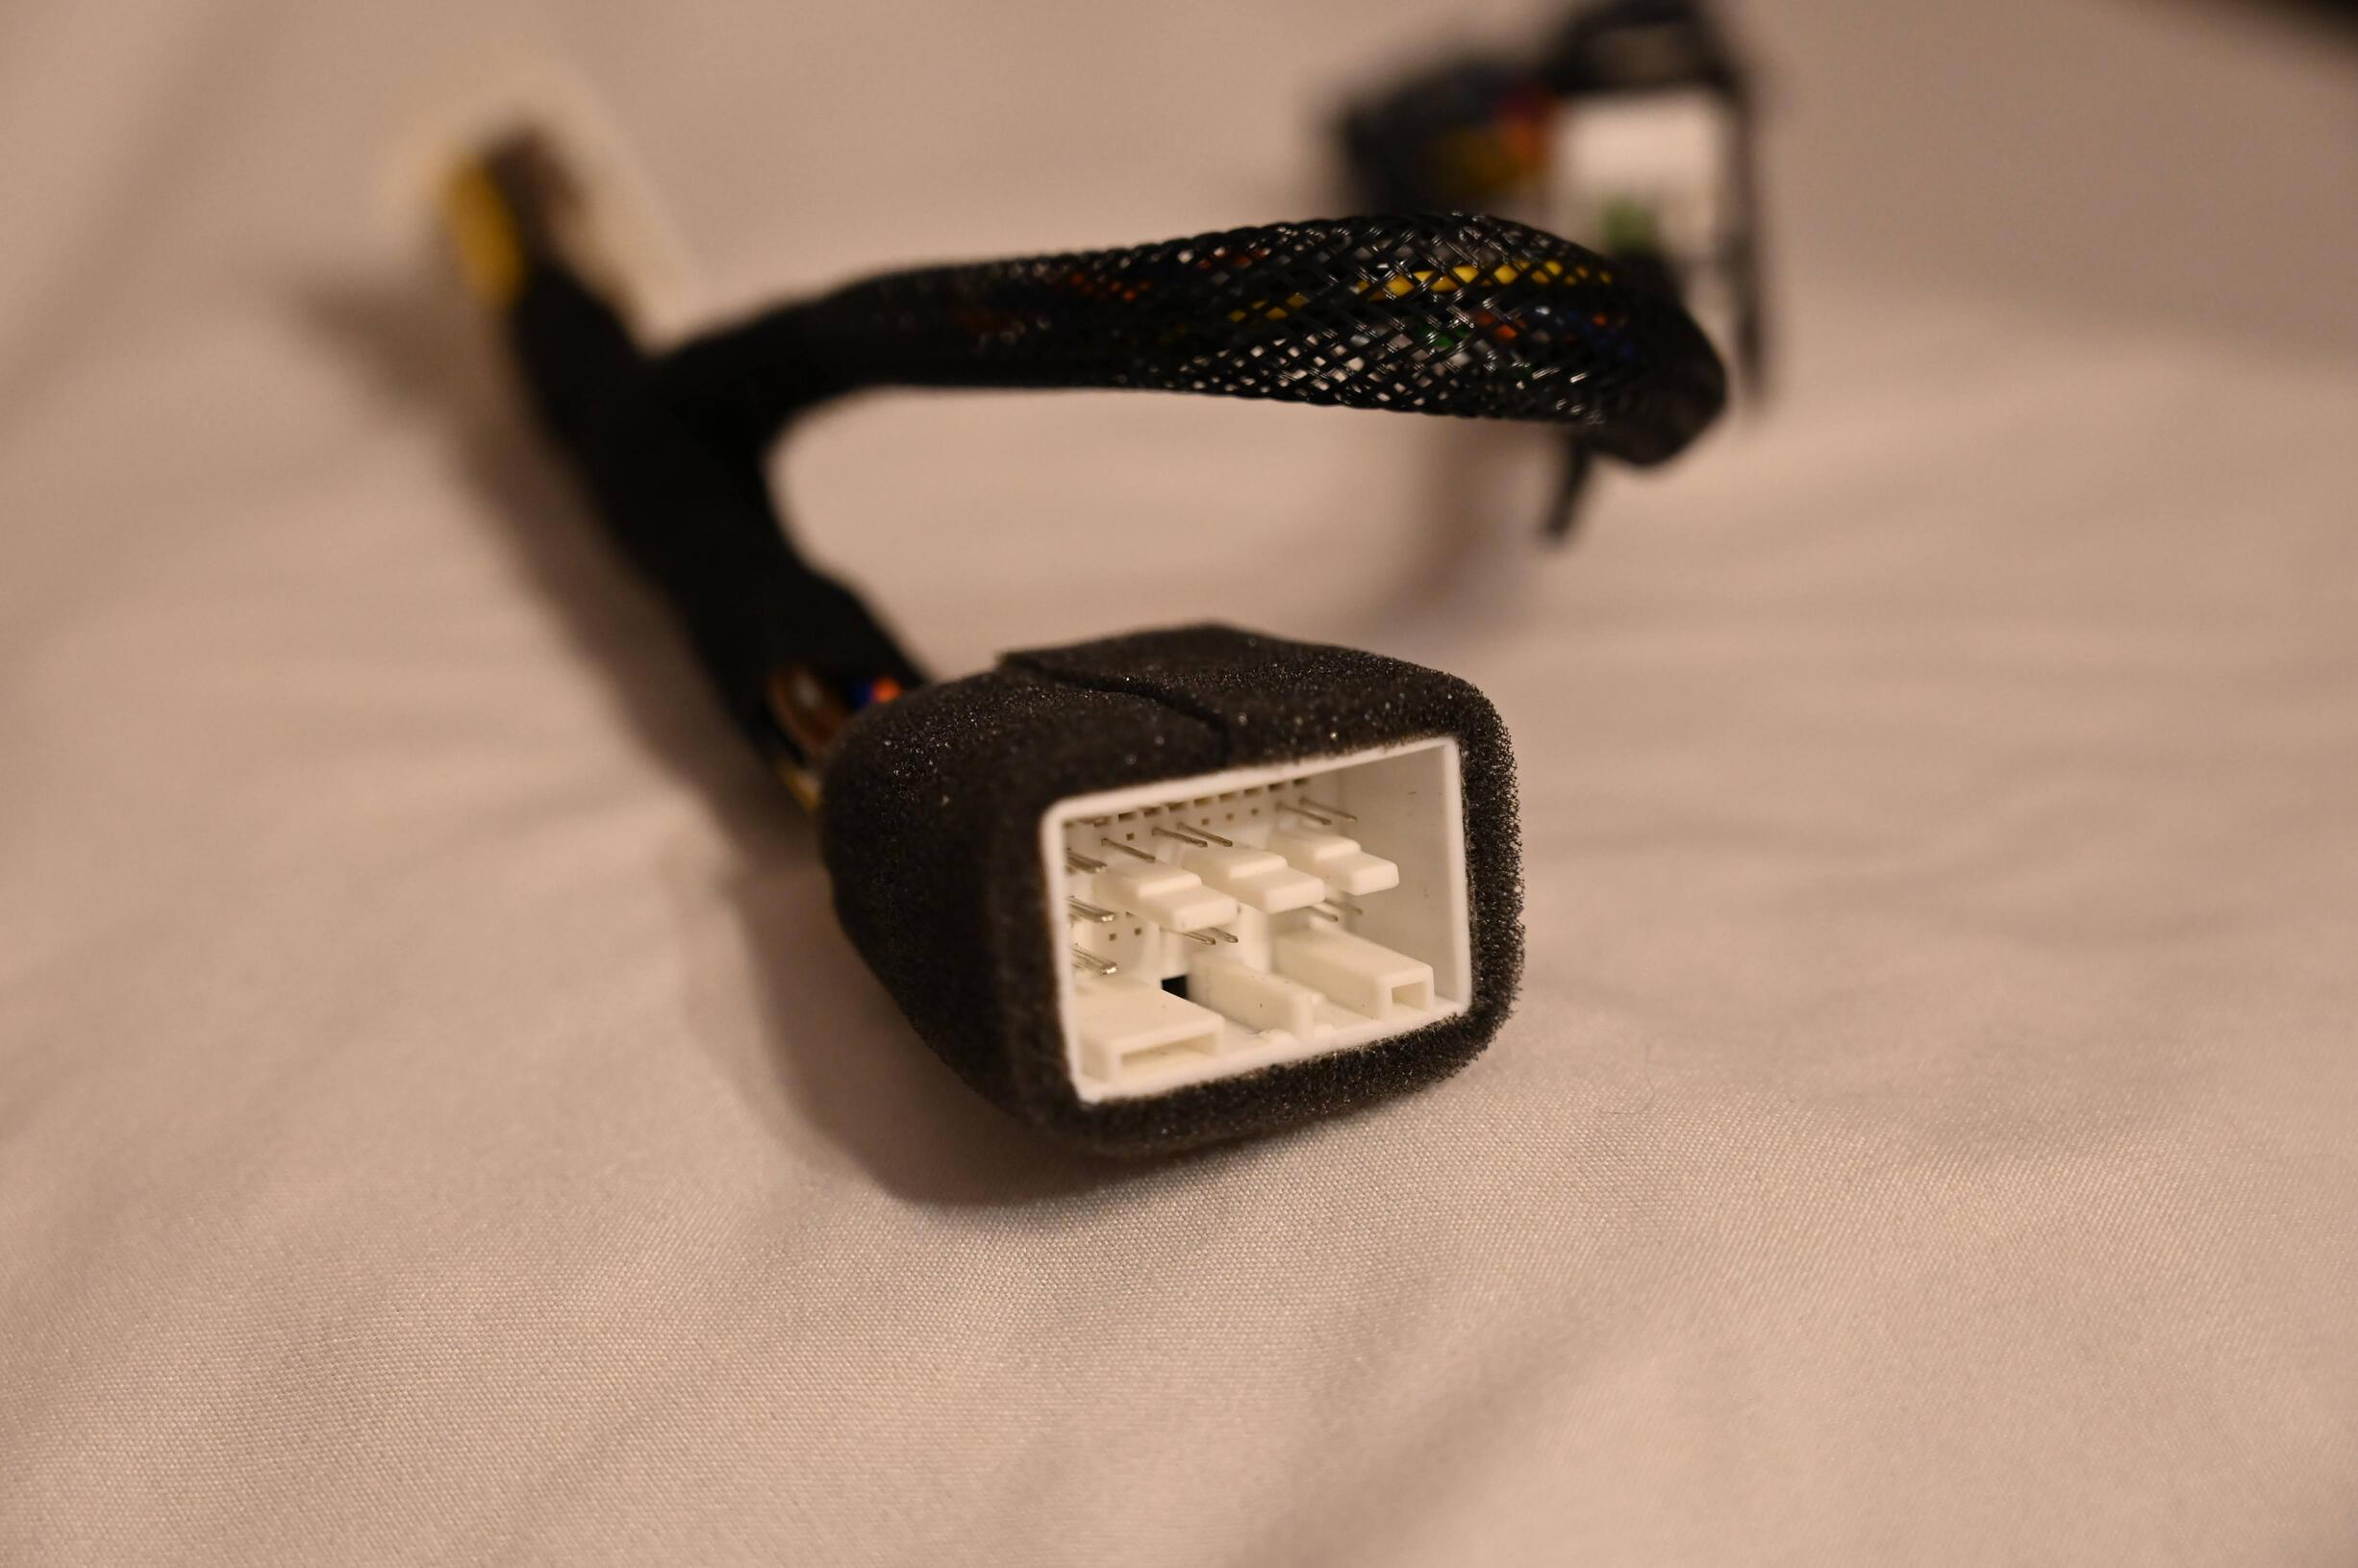
\includegraphics[height=1.5in,angle=0]{photos/male_harness_end.jpg} }  \\
  \subfloat[]{\label{subfig:harness:headunit}
  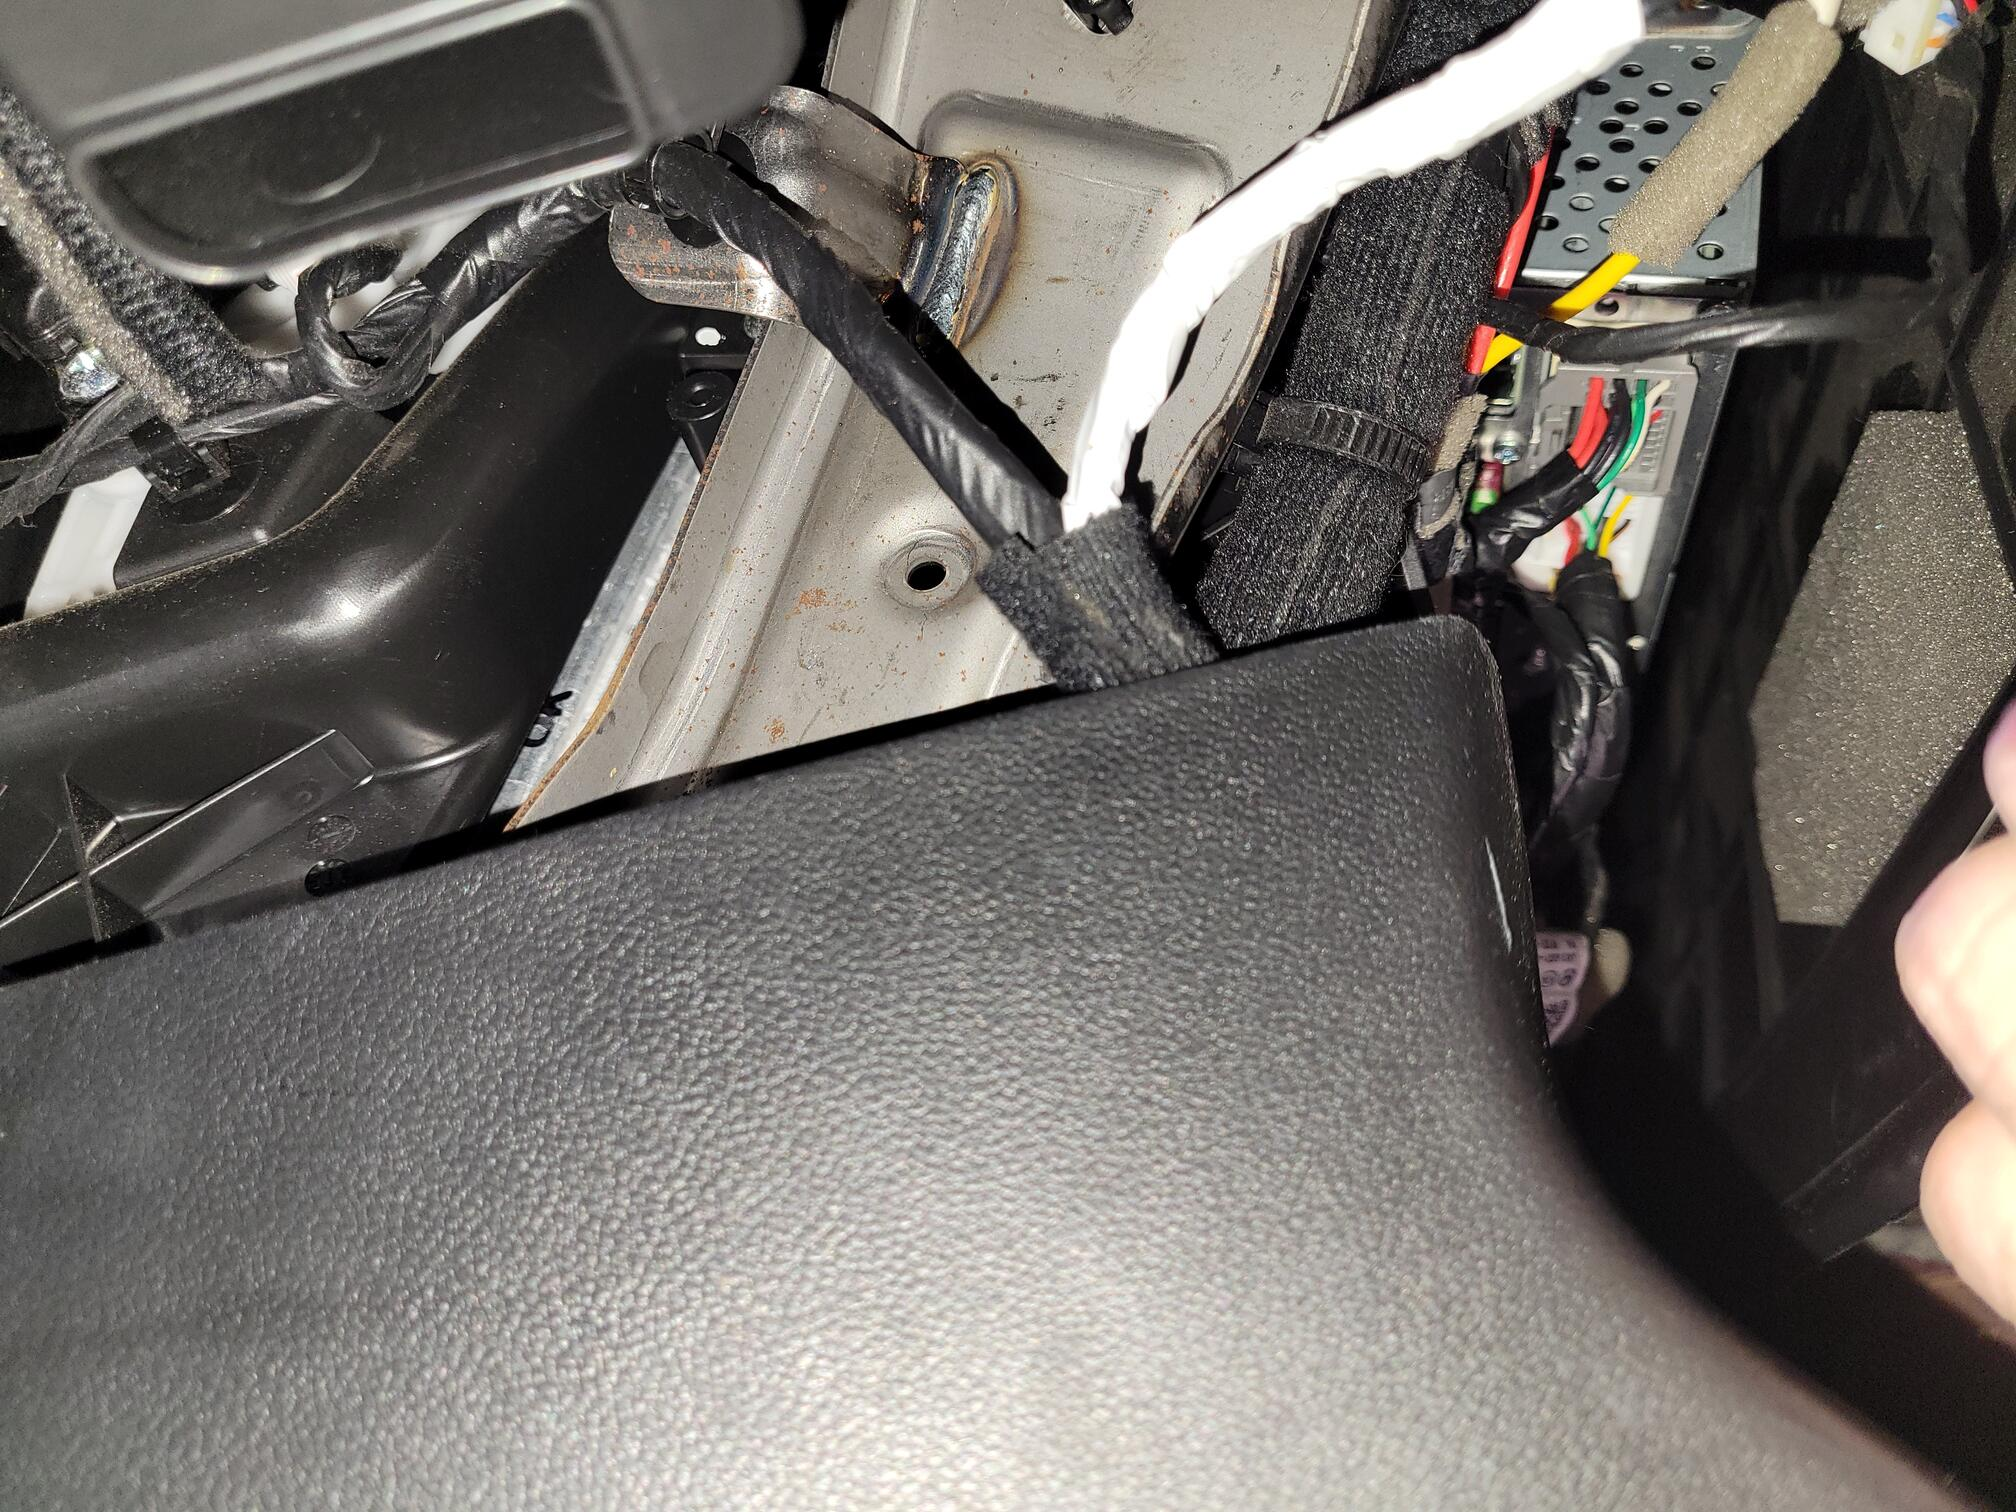
\includegraphics[height=1.5in,angle=0]{photos/head_unit_connectors_in.jpg} } 
  \subfloat[]{\label{subfig:harness:M05Bout}
  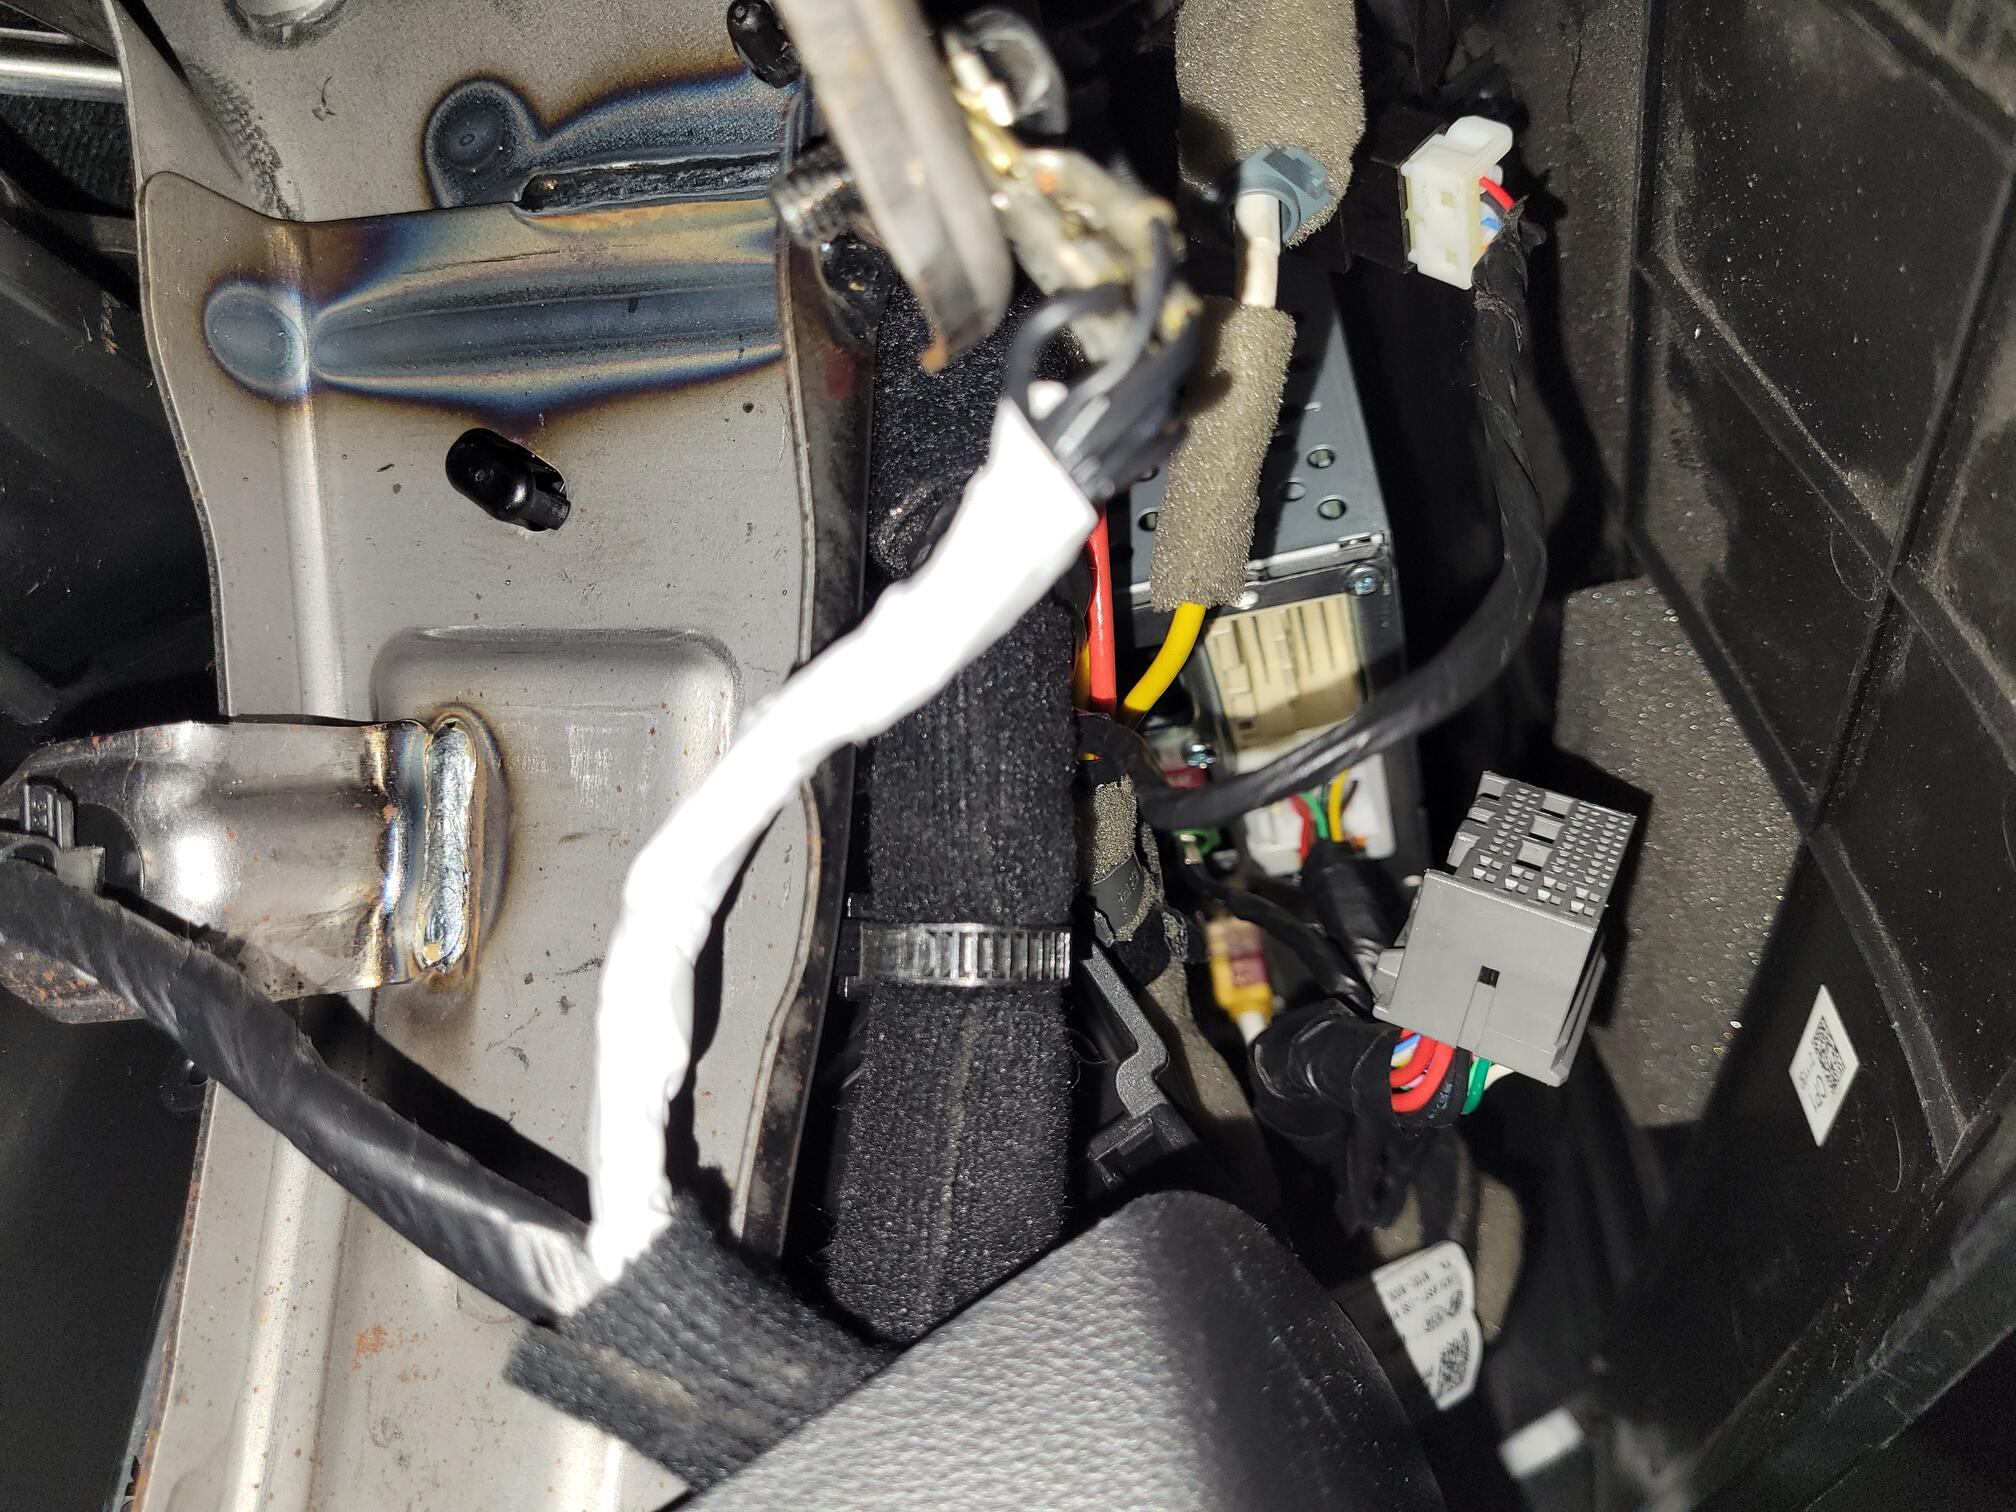
\includegraphics[height=1.5in,angle=0]{photos/M05-B_out.jpg} } 
  \subfloat[]{\label{subfig:harness:harness_in}
  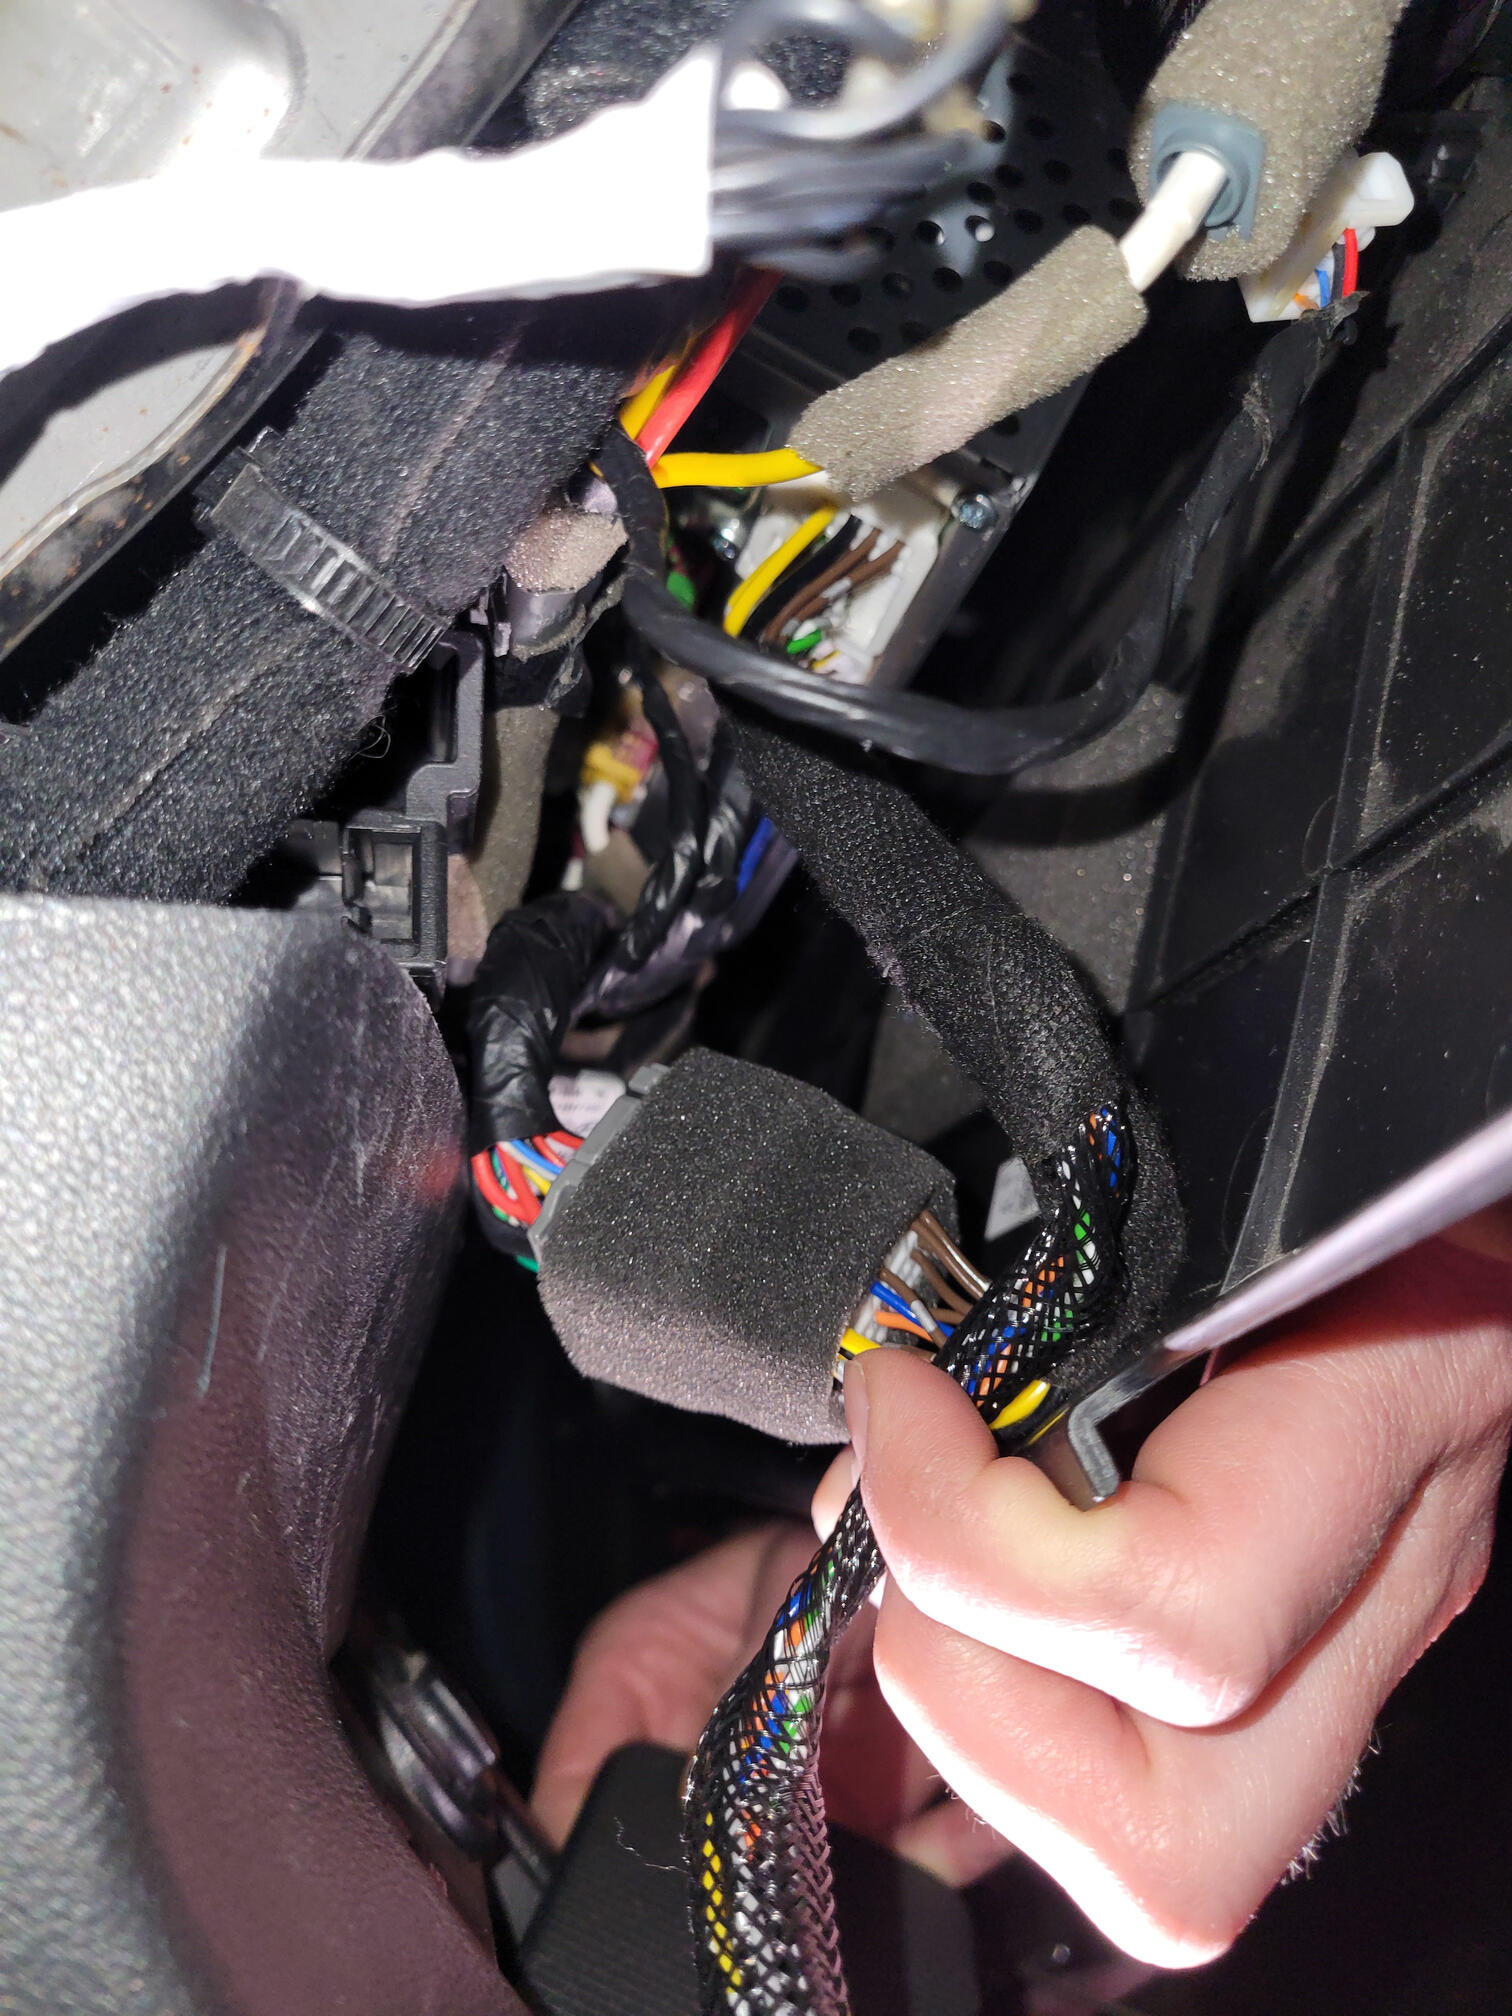
\includegraphics[height=1.5in,angle=0]{photos/harness_in.jpg} }  
   \caption{(a) Photo étiquetée montrant le connecteur de faisceau femelle. (b) Connecteur de faisceau mâle. (c) Unité principale avec connecteurs branchés. (d) Connecteur femelle M05-B (gris) retiré de l'unité principale. (e) Harnais installé dans l'unité principale. \label{fig:harness}}
\end{figure}
\section{Étape 4 : Montage OBD} \label{sect:3}
Dans cette étape, nous montons solidement l’extrémité OBD du faisceau et branchons le WiCAN. 

Instructions étape par étape :
\begin{enumerate}
  \item Enfiler le harnais le long du bord inférieur du crash pad inférieur
  \item Branchez la femelle OBD dans le support
  \item Utilisez du ruban adhésif double face pour fixer le support sur le côté de l'aération de l'espace pour les pieds, derrière le bas du coussin de protection (Figure \ref{subfig:obd:wican})
  \item Utilisez des attaches zippées pour attacher le faisceau à d'autres fils et points de montage (Figure \ref{subfig:obd:zip_tie} et \ref{subfig:obd:zip_tie2})
  \item Tout en tenant le support, branchez le WiCAN (Figure \ref{subfig:obd:wican})
\end{enumerate}

\begin{figure}[h]
  \subfloat[]{\label{subfig:obd:zip_tie}
  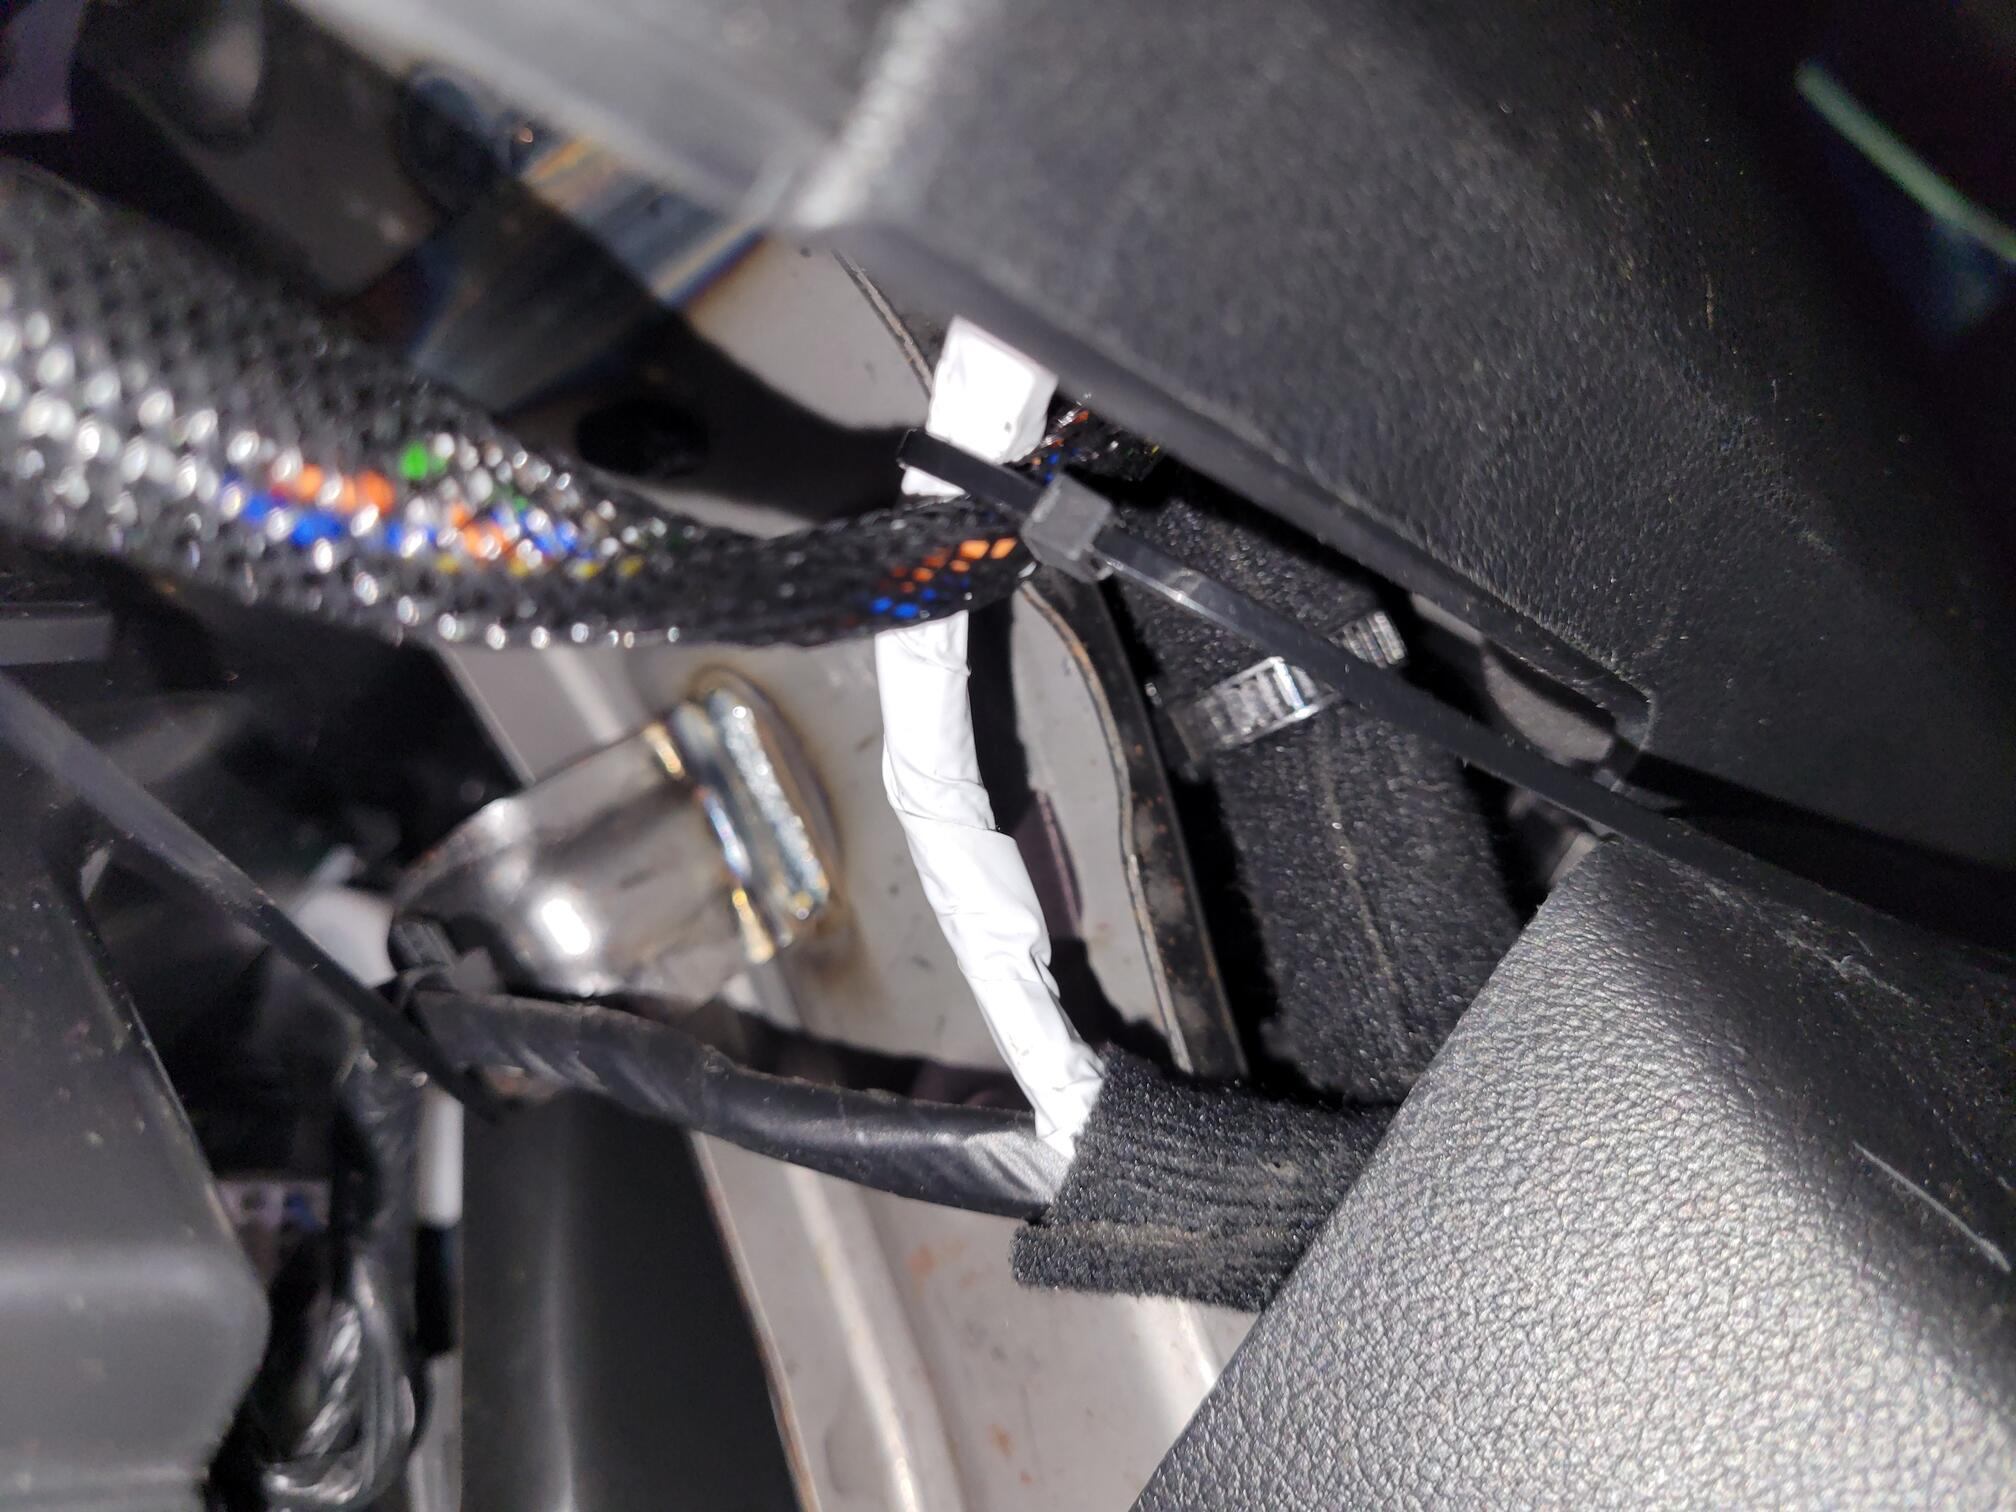
\includegraphics[height=1.5in,angle=0]{photos/zip_tie_1.jpg} } 
  \subfloat[]{\label{subfig:obd:zip_tie2}
  \includegraphics[height=1.5in,angle=0]{photos/harness_mounted_zip_ties_2.jpg} } 
  \subfloat[]{\label{subfig:obd:wican}
  \includegraphics[height=1.5in,angle=0]{photos/WiCAN_installed_on_vent.jpg} } 
   \caption{(a) Harnais attaché au fil existant. (b) Harnais attaché avec une fermeture éclair au support de ventilation. (c) WiCAN monté sur le côté de l'évent. \label{fig:obd}}
\end{figure}

\section{Étape 5 : Nettoyer} \label{sect:4}
Inversez les étapes de retrait des garnitures. Assurez-vous que les clips de garniture sont alignés, puis remettez fermement les panneaux de garniture en place. Rebranchez la borne négative de la batterie 12 V. Le WiCAN devrait immédiatement afficher une lumière bleue. Changez votre mot de passe WiCAN : \href{https://meatpihq.github.io/wican-fw/config/wifi}{https://meatpihq.github.io/wican-fw/config/wifi}. Vous pouvez connecter votre WiCAN directement en trouvant un réseau WiFi nommé 'WiCAN\_xxxxxxx' et je vais à \href{http://192.168.80.1/}{http://192.168.80.1/} dans votre navigateur.
\appendix 
\end{document}